\chapter{Method and Results}
\label{ch:Method_and_Result}

\section{Factorization Machine with Annealing Optimization Framework}
本研究採用的最佳化方法為 Factorization Machine with Annealing Optimization。
這個方法主要是參考 Kitai 等人於 2020 年提出之 \textit{Designing Metamaterials with Quantum Annealing and Factorization Machines}\cite{kitai2020_fmqa}。
此研究建立了一個結合因子分解機(Factorization Machine)與量子退火(Quantum Annealing)的 FMQA 架構，
透過 因子分解機 建立目標函數的代理模型，並將其轉換為二元二次最佳化問題，再利用量子退火搜尋候選設計。

然而，本研究並沒有直接使用量子退火作為 QUBO 求解器，而是採用模擬退火(Simulated Annealing, SA)進行候選結構搜尋。
因此，本研究保留了 FMQA 架構中「FM 代理模型、QUBO 轉換與退火搜尋」的核心流程，並以 SA 取代原始架構中的 QA，
將其應用於反向設計。

在本章節中我會說明Factorization Machine with Annealing Optimization 的架構以及實際的完整執行流程。
首先我會介紹初始結構資料集的建立方式，接著說明 FM 代理模型之訓練，以及其模型參數轉換為 QUBO 問題的流程。
然後，我會說明本研究如何使用 SA 求解 QUBO 問題，以產生具潛力之候選結構。
最後，我將介紹候選結構經過解碼與 FDTD 模擬評估後，如何回饋至訓練資料集，並透過重複訓練與搜尋一步一步完成結構最佳化。
另外，不同結構編碼策略的設計與實作方式也不盡相同，因此我會於後續章節中進一步說明。

Factorization Machine with Annealing Optimization 整體流程如圖~\ref{fig:FMSA_flowchart}所示，
主要流程可概分為下列步驟:
\begin{figure}[htb]
\centering
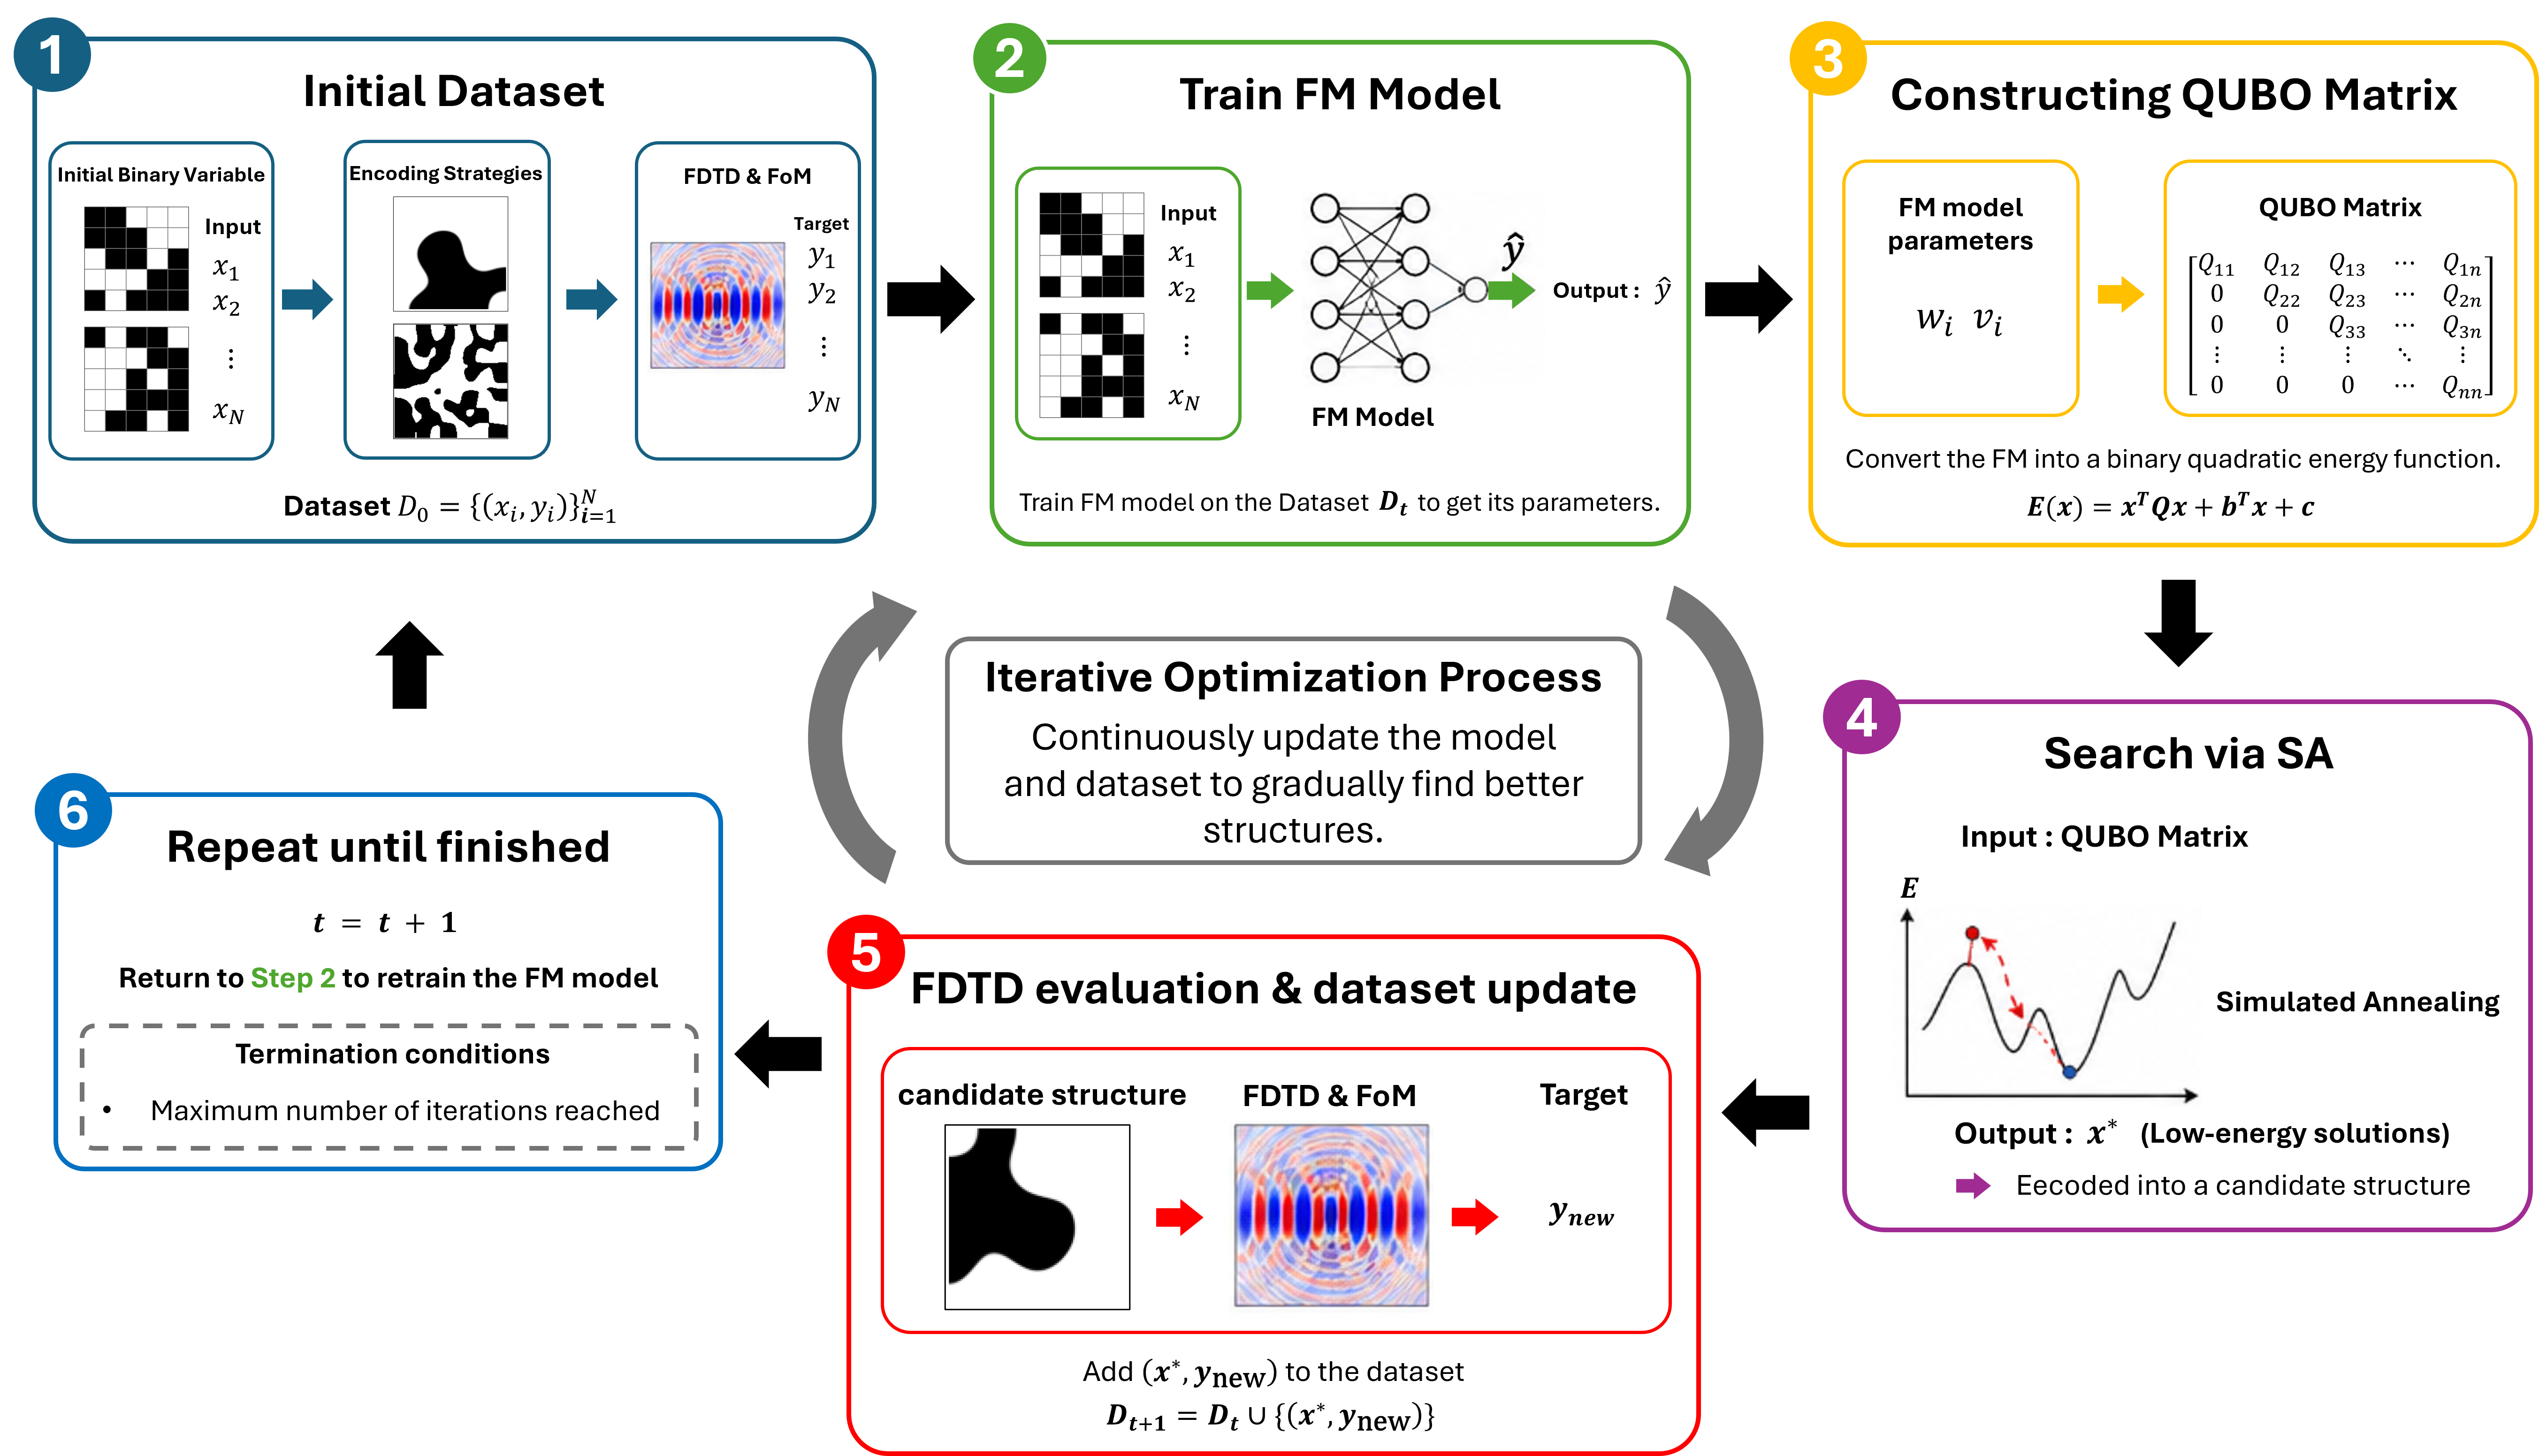
\includegraphics[width=1.0\textwidth]{img/FMSA_flowchart.png}
\caption{Factorization Machine with Annealing Optimization 整體流程圖。}
\label{fig:FMSA_flowchart}
\end{figure}

\noindent \textbf{一、建立初始訓練資料集 (Initial Dataset Generation)}\\
一開始會先隨機產生一組初始隨機二元變數(Initial Random Binary Variables)$x_i$，這些二元變數是沒有經過任何結構約束或模型訓練的。
接著我們會透過特定的編碼策略(Encoding Strategies)來對初始二元變數進行編碼(Encoding)，
這時候我們就會得到一組平滑化後的二維結構圖。
接著，針對這些隨機二元變數編碼後的二維結構圖，利用有限時域差分法(Finite-Difference Time-Domain, FDTD)進行電磁模擬，
取得其光學效率，例如特定波長下的傳輸率。再根據模擬結果計算品質因子(Figure of Merit, FoM)，這邊我們可以記為 $y_i$。
最終可建立包含 $N$ 筆資料的初始訓練資料集$D_0$:
\begin{align}
D_0={(x_i,y_i)}_{i=1}^{N}.
\end{align}
此資料集會作為後續模型訓練的基礎。

\noindent \textbf{二、訓練因子分解機代理模型（Training the FM Surrogate Model）}\\
為了降低直接透過 FDTD 模擬龐大設計空間所需的計算成本，在研究中採用因子分解機(Factorization Machine, FM)作為代理模型。
將第一步所建立的初始訓練資料集 $D_0$ 中的隨機設計變數$x_i$與對應 FoM $y_i$ 輸入 因子分解機 進行監督式訓練，
使模型學習設計變數中每個矩陣元素與光學性能之間的關係。

訓練完成後，因子分解機 可以得到線性權重 $w_i$ 與二階交互作用參數 $v_i$。
其中，二階項 $v_i$ 用來描述不同結構變數間的交互作用，並作為下一步用來轉換為 QUBO 問題的依據。

\noindent \textbf{三、建構無約束二元二次最佳化問題(Constructing the QUBO Problem)}\\
根據訓練完成的因子分解機模型參數，可以將預測函數 $\hat{y}$ 轉換為無約束二元二次最佳化(Quadratic Unconstrained Binary Optimization, QUBO)形式。
經過轉換後，目標能量函數可以表示為：
\begin{align}
E(x)=x^{T}Qx+b^{T}x+c,
\end{align}
其中，$Q$ 為二次交互作用矩陣，$b$ 為線性項，$c$ 為常數項。
如果設計目標是最大化元件的傳輸率或 FoM，我們可以在程式中調整目標函數的正負號，讓最大化問題可以隨著最小化能量函數 $E(x)$降低而降低。

\noindent \textbf{四、以模擬退火演算法搜尋候選結構(Candidate Structure Search via SA)}\\
將 QUBO 問題輸入模擬退火(Simulated Annealing)演算法進行求解。SA 透過隨機擾動與逐步降溫等機制來進行採樣，以探索出它認為最有潛力的二元設計變數，
並且可降低搜尋過程陷入局部最佳解的機率。
求解完成後，就可以得到預測出的一組二元設計變數 $x^{*}$。

接著，預測出的二元設計變數會依照不同的編碼策略再轉換為其對應的二維光學結構圖，來作為下一步 FDTD 模擬的候選結構。

\noindent \textbf{五、FDTD 評估與資料集更新(FDTD Evaluation and Dataset Update)}\\
將 SA 搜尋得到的候選結構輸入 FDTD 模擬，以用來計算其光學性能及目標函數值 $y_{\mathrm{new}}$。
完成模擬後，將新結構 $x^*$及其對應 FoM $y_{new}$ 加入原本的資料集 $D_t$，得到更新後的訓練資料集 $D_{t+1}$:
\begin{align}
D_{t+1}=D_t\cup{(x^{*},y_{\mathrm{new}})}.
\end{align}
透過持續迭代並加入高光學性能的結構資料集，可以提升因子分解機模型的預測能力。

\noindent \textbf{六、重複迭代至終止條件(Iterative Optimization Process)}\\
上述的步驟可以構成一個閉環式的最佳化流程。
在每次資料集$D_t$更新後，重新訓練 因子分解機 模型，並重複執行 QUBO 建構、SA 搜尋與 FDTD 模擬驗證。
隨著迭代的進行，資料集$D_t$會慢慢增加 良好 FoM 的資料，使因子分解機 模型能夠更有效的在設計空間中引導搜尋方向。
當達到程式預設的最大迭代次數(例如100次)時，將會停止整個最佳化的流程。

\section{Encoding Strategies for Factorization Machine with Annealing Optimization}
在因子分解機結合模擬退火的架構中，結構表示方式會直接影響因子分解機作為代理模型的訓練效率、QUBO 問題的維度，
以及模擬退火的搜尋範圍。若直接將設計區域中每一個像素作為獨立設計變數，雖然可保留光學結構的完整資訊，
但隨著設計區域解析度的提高，設計變數數量將會大幅增加，
導致因子分解機模型訓練、QUBO 矩陣建構與模擬退火求解的計算成本也會大幅上升。

如第~\ref{ch:Encoding_Strategies_Theory} 節中所述，此篇論文已說明各編碼策略的相關理論基礎。
接著，在本小節中將進一步介紹 Gaussian Upsampling Strategy、2D Fourier Integral Strategy 與
 $\beta$-Variational Autoencoder ($\beta$-VAE) Strategy 這三種編碼策略的具體實作方法以及
其於 因子分解機 結合模擬退火架構中的運作流程。

\subsection{Gaussian Upsampling Strategy}
\label{ch:Gaussian_Upsampling_Strategy}
在前一節說明的 因子分解機 結合模擬退火架構中，設計變數的表示方式會直接影響搜尋空間大小與最佳化的效率。
因此，本小節將介紹利用 Gaussian Upsampling Strategy 作為二維光學結構的編碼方法，此編碼策略以低維二元矩陣作為設計變數，
並透過 Gaussian convolution、Tanh projection 與 MaterialGrid mapping 等步驟將其轉換為高解析度的物理結構，
使最佳化過程能於較低維度的搜尋空間中進行，並同時維持結構邊界的平滑性與製程可行性。

\subsubsection{Flowchart}
Gaussian Upsampling Strategy 的整體流程如圖 \ref{fig:Gaussian_Upsampling_Flowchart} 所示，
其中主要包含了低維設計變數重建、高斯卷積平滑、Tanh 投影以及 MaterialGrid 建立等四個步驟。
\begin{figure}[htb]
\centering
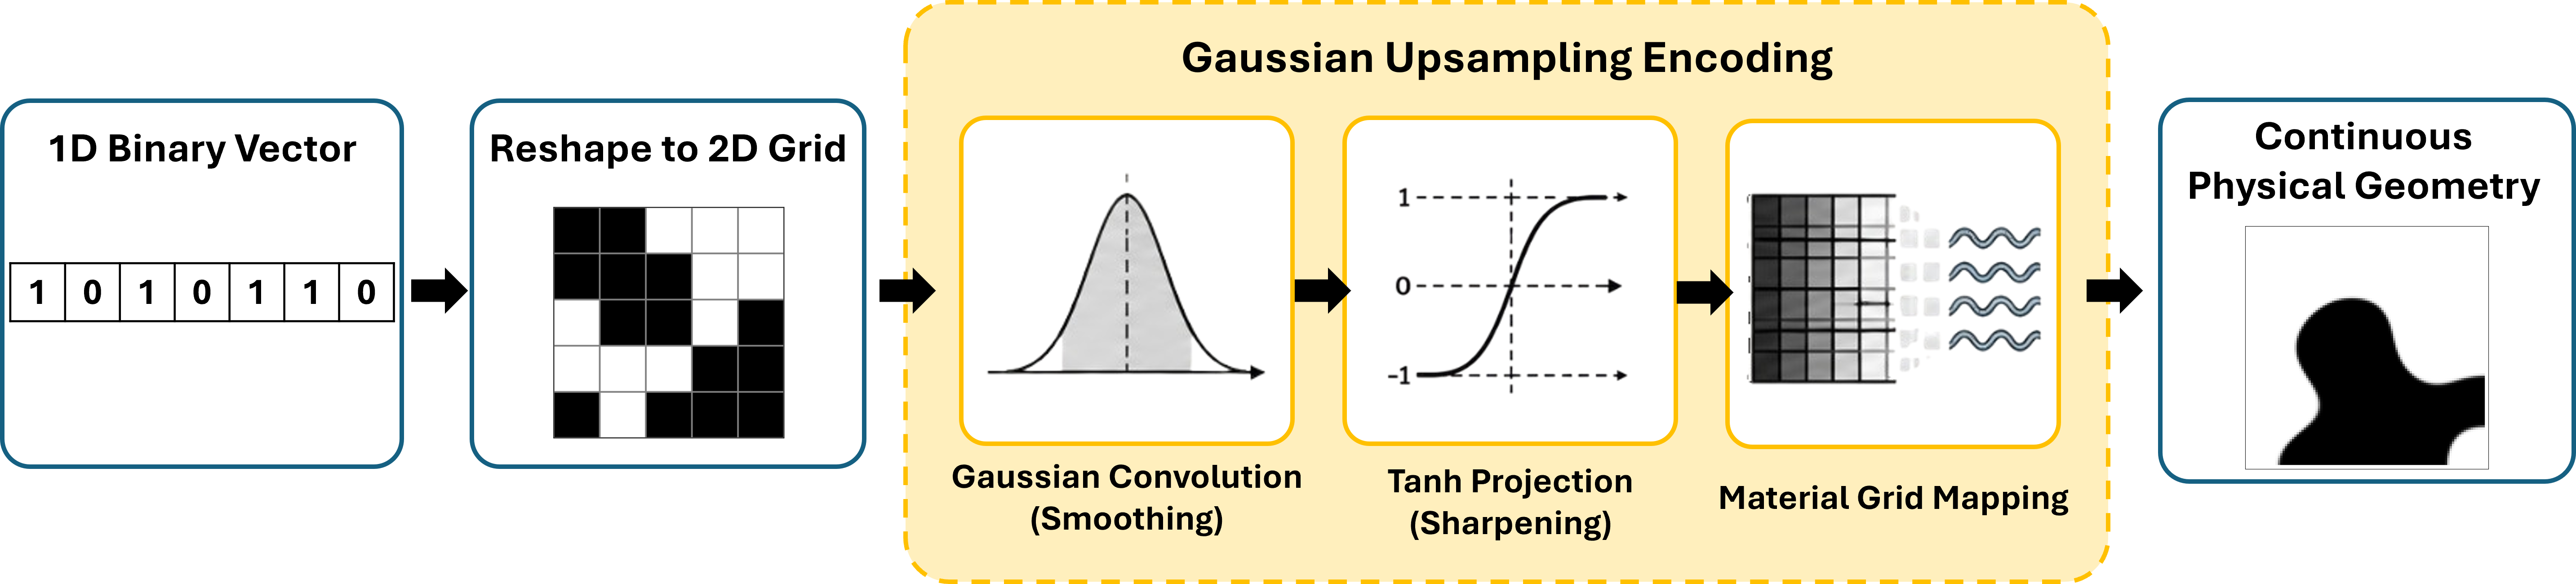
\includegraphics[width=1.0\textwidth]{img/GU_flowchart.png}
\caption{高斯上採樣(Gaussian Upsampling)流程圖。}
\label{fig:Gaussian_Upsampling_Flowchart}
\end{figure}

在初始資料集建立階段，首先隨機產生 $i$ 組低維二元結構。
此研究設定每組結構由 $N \times N$ 的二元矩陣表示，因此每一組樣本包含 $N^2$ 個二元設計變數。
為了避免初始樣本產生過多沒有物理意義的隨機雜訊，會在隨機生成過程中加入平滑濾波處理，使初始結構具有較連續的幾何特徵。

首先，以 Gaussian kernel 對低維矩陣進行卷積運算，將原始二元分布轉換為連續密度場，以降低像素化結構所造成的鋸齒狀邊界以及局部孤島或尖角，
使材料分布具有空間連續性。

接著，利用Tanh projection將連續密度場重新映射為接近二元的材料分布。在這個步驟除了可以保留平滑邊界，
也可以提高介面的清晰度，使生成出的光學結構具有可製造與可實現性。

完成 Gaussian Upsampling 編碼後，可以得到對應的高解析度密度矩陣。
接著，所得的密度矩陣會丟給 MEEP 的 MaterialGrid 中，用來建立其對應的介電常數分佈，
也就是正式把二維光學結構與材料分布建構出來。最後透過 MEEP(FDTD) 進行電磁模擬，
就可以得到每組低維二元設計變數$x_i$所對應的光學性能與品質因子$y_i$(Figure of Merit, FoM)。

在後續最佳化迭代過程中，因子分解機(FM)模型與模擬退火演算法皆於低維二元設計空間中進行搜尋。
每當模擬退火採樣出新的候選解$x^*$時，這些候選解就會再次透過相同的 Gaussian Upsampling 流程轉換為高解析度結構，
並輸入 MEEP 進行驗證。透過此機制，Gaussian Upsampling 在最佳化流程中扮演低維設計變數與實際物理結構之間的轉換橋樑。

相較於直接以高解析度像素作為設計變數，此方法可以大幅降低 QUBO 問題維度，同時透過高斯平滑與投影機制限制結構邊界變化，
使最佳化結果更符合實際製程需求。

\subsubsection{Fabrication Constraints}
雖然 Gaussian Upsampling 可將低維二元設計變數轉換為連續的幾何結構，但若未納入實際製程限制，
最佳化的結果還是有可能會出現窄波導、尖角或孤島區域等難以製造的物理特徵。
因此，本研究中利用 Gaussian filter 的空間平滑特性來控制結構的最小特徵尺寸(Minimum Feature Size, MFS)，
使生成之光學結構可以符合預期的製程限制。

由第~\ref{ch:GU_theory}節中的公式\eqref{eq:b_min}可知:
\begin{align}
\sigma_{\text{pix}} \ge \frac{b_{\text{fab}}}{1.35d}
\label{eq:sigma_pix_min}
\end{align}
其中，$b_{\text{fab}}$為製程允許的最小線寬(Minimum Feature Size, MFS)，
$d$為單一網格(pixel)所對應的物理尺寸，而$\sigma_{\text{pix}}$為高斯濾波器的標準差。

為了避免Gaussian Kernel遭到截斷，高斯核卷積核的視窗大小必須滿足:
\begin{align}
W \ge 6\sigma_{\text{pix}} + 1
\label{eq:gaussian_kernel_size}
\end{align}
並且取奇數。

因此，假設設計區域為
\begin{align}
5 \mu m \times 5 \mu m,
\end{align}
且其二元設計變數為$50 \times 50$，則我們可以計算出$d$:
\begin{align}
d = 100 nm
\end{align}
若製程要求為:
\begin{align}
b_{fab} = 150 nm
\end{align}
則
\begin{align}
\sigma_{pix} = \frac{150}{1.35 \times 100} \approx 1.11
\end{align}
因此我們可以透過設定$\sigma_{pix}=1.11$以及$W=7$來滿足製程限制$\ge 150 nm$。

為方便實際參數設定，本研究整理不同製程限制與設計網格下所對應之$\sigma_{\text{pix}}$與$W$，如Table~\ref{tab:kernel_parameter} 所示。
\begin{table}[H]
\centering
\begin{tabular}{cccc}
\hline
Grid size & Target MFS & $\sigma_{\text{pix}}$ & $W$ \\ \hline
50 nm     & 100 nm     & 1.48                               & 9   \\
50 nm     & 120 nm     & 1.78                               & 11  \\
100 nm    & 120 nm     & 0.89                               & 5   \\
100 nm    & 150 nm     & 1.11                               & 7   \\
100 nm    & 200 nm     & 1.48                               & 9   \\ \hline
\end{tabular}

\captionsetup{name=TABLE, font={color=blue, sf, footnotesize}}
\caption{不同製程限制下 Gaussian Filter 之設計參數對照表。}
\label{tab:kernel_parameter}
\end{table}
從Table~\ref{tab:kernel_parameter} 可知，隨著目標最小線寬增加，所需的 Gaussian 標準差也必須提高，
以增強平滑效果並抑制較小的幾何特徵。
另一方面，由於過小的 Gaussian 標準差會使濾波器的平滑效果有限，並可能會降低對部分幾何特徵的約束能力，
因此當$\sigma_{\text{pix}} < 1$時，應該將$\sigma_{\text{pix}}$調整為$1$。

\subsection{2D Fourier Integral Strategy}
接著，我將會說明2D Fourier Integral這套編碼策略的運作流程，如圖~\ref{fig:2D_fourier_flowchart}所示。
\begin{figure}[H]
\centering
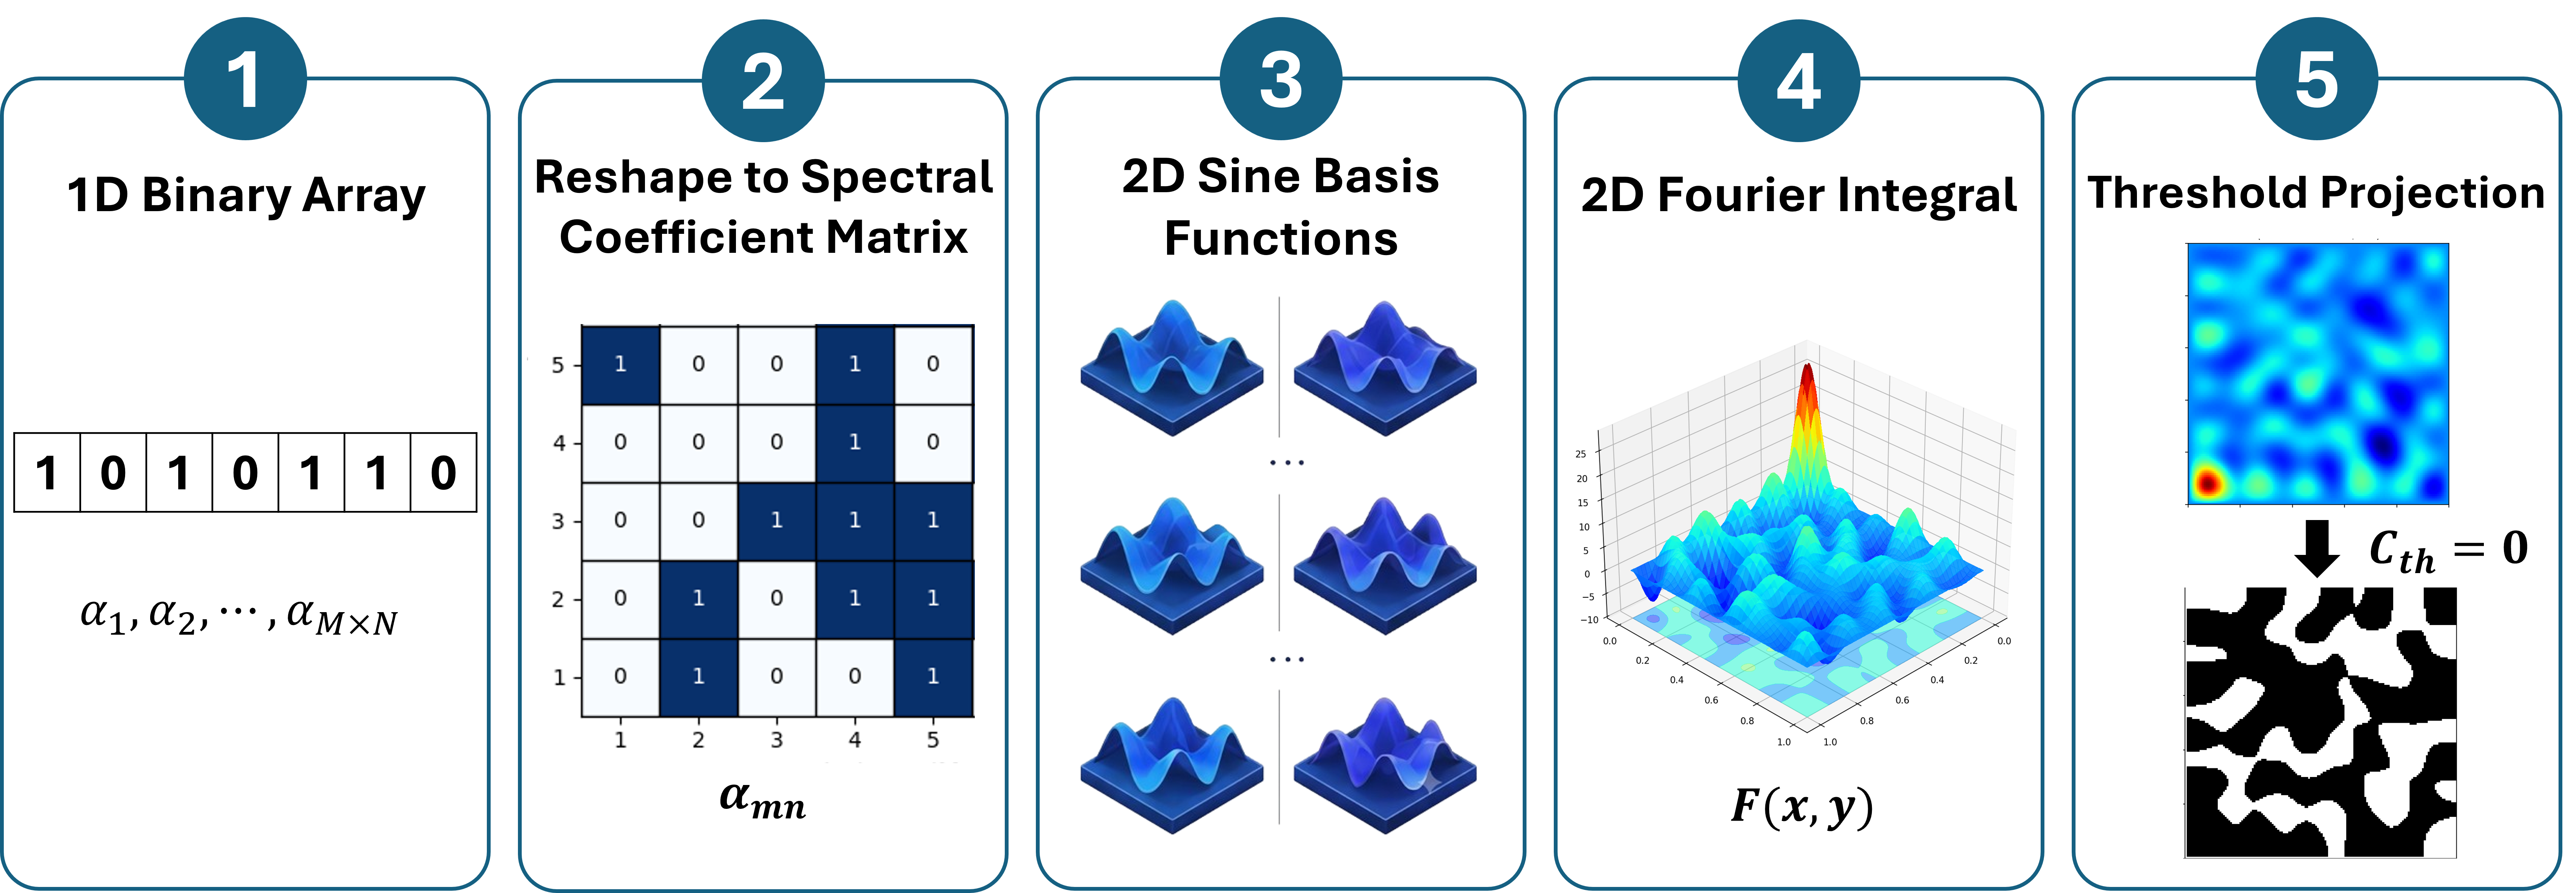
\includegraphics[width=1.0\textwidth]{img/2D_fourier_flowchart.png}
\caption{2D Fourier Integral編碼策略之整體流程圖。}
\label{fig:2D_fourier_flowchart}
\end{figure}

首先，輸入數量為 $M \times N$ 的二元陣列 $\boldsymbol{\alpha}_{M \times N}$，此陣列會在初始隨機生成階段或模擬退火階段透過採樣產生。
這邊假設以 $8 \times 8$ 的頻譜設定為例，輸入陣列包含 $64$ 個二元變數，可表示為:
\begin{align}
\alpha_1,\alpha_2,\ldots,\alpha_{64}
\qquad
\alpha_i \in {0,1}
\end{align}

將一維陣列重建為至二維的頻率係數矩陣$\alpha_{mn}$ ，其中的每個元素決定對應空間頻率模態是否會參與結構的生成。
接著，在設計區域內建立歸一化空間，座標為 $(x,y)$，其中 $x,y\in[0,1]$，其取樣解析度設定為最終模擬結構的網格大小。
連續疊加場$\boldsymbol{F}(x,y)$可透過各個頻率的模態疊加表示為:
\begin{align}
\boldsymbol{F}(x,y) = \sum_{m=1}^{M}
\sum_{n=1}^{N}
\alpha_{mn}
\sin(m\pi x)
\sin(n\pi y)
\label{eq:2D_fourier_mode_summation}
\end{align}

由公式 \eqref{eq:2D_fourier_mode_summation} 可以得到連續的二維空間場，
其中不同二元設計變數$\alpha_{mn}$的組合會決定各頻率成分的疊加結果，進而導致二維連續疊加場的不同。

接著會將二維連續疊加場透過閾值 $C_{\mathrm{th}}$ 進行二值化，以將其轉換為二元材料分佈。

在本研究中設定 $C_{\mathrm{th}}=0$。
因為設計出的結構邊界是透過有限數量的正弦模態疊加後再經閾值進行二值化，因此與直接以二元像素表示結構的方法相比，
此方法可以產生較為連續的幾何邊界，減少像素化的鋸齒邊界。

完成二值化後會將 $\rho(x,y)$ 輸入 MEEP 的 MaterialGrid，並以 MaterialGrid 功能來建立設計區域的材料分佈，
其中，$\rho(x,y)=1$ 代表高折射率材料區域，此研究中使用矽(Si)，$\rho(x,y)=0$ 則代表低折射率的背景預設材料，此研究中使用二氧化矽(SiO$_2$)。
最後，將此設計區域與輸入及輸出波導結構結合，作為 FDTD 模擬中的幾何模型，以用來計算其光學性能與其對應的 FoM。

在 FM 模型結合模擬退火的最佳化流程中，FM 模型的輸入為頻譜二元向量 $\boldsymbol{\alpha}_{M \times N}$。
當模擬退火採樣出新的頻譜向量後，會透過相同的編碼程序重新建構候選結構，再透過 FDTD 模擬進行驗證。

\subsection{$\beta$-Variational Autoencoder ($\beta$-VAE) Strategy}
接著，在此小節我將說明 $\beta$-Variational Autoencoder($\beta$-VAE)編碼策略的運作流程，
如圖~\ref{fig:bVAE_flowchart} 所示。此方法主要用於處理高解析度二維結構所造成的高維度設計問題，
並將原始結構壓縮至較低維度的二元潛在空間，以降低後續模擬退火的搜尋難度。
\begin{figure}[H]
\centering
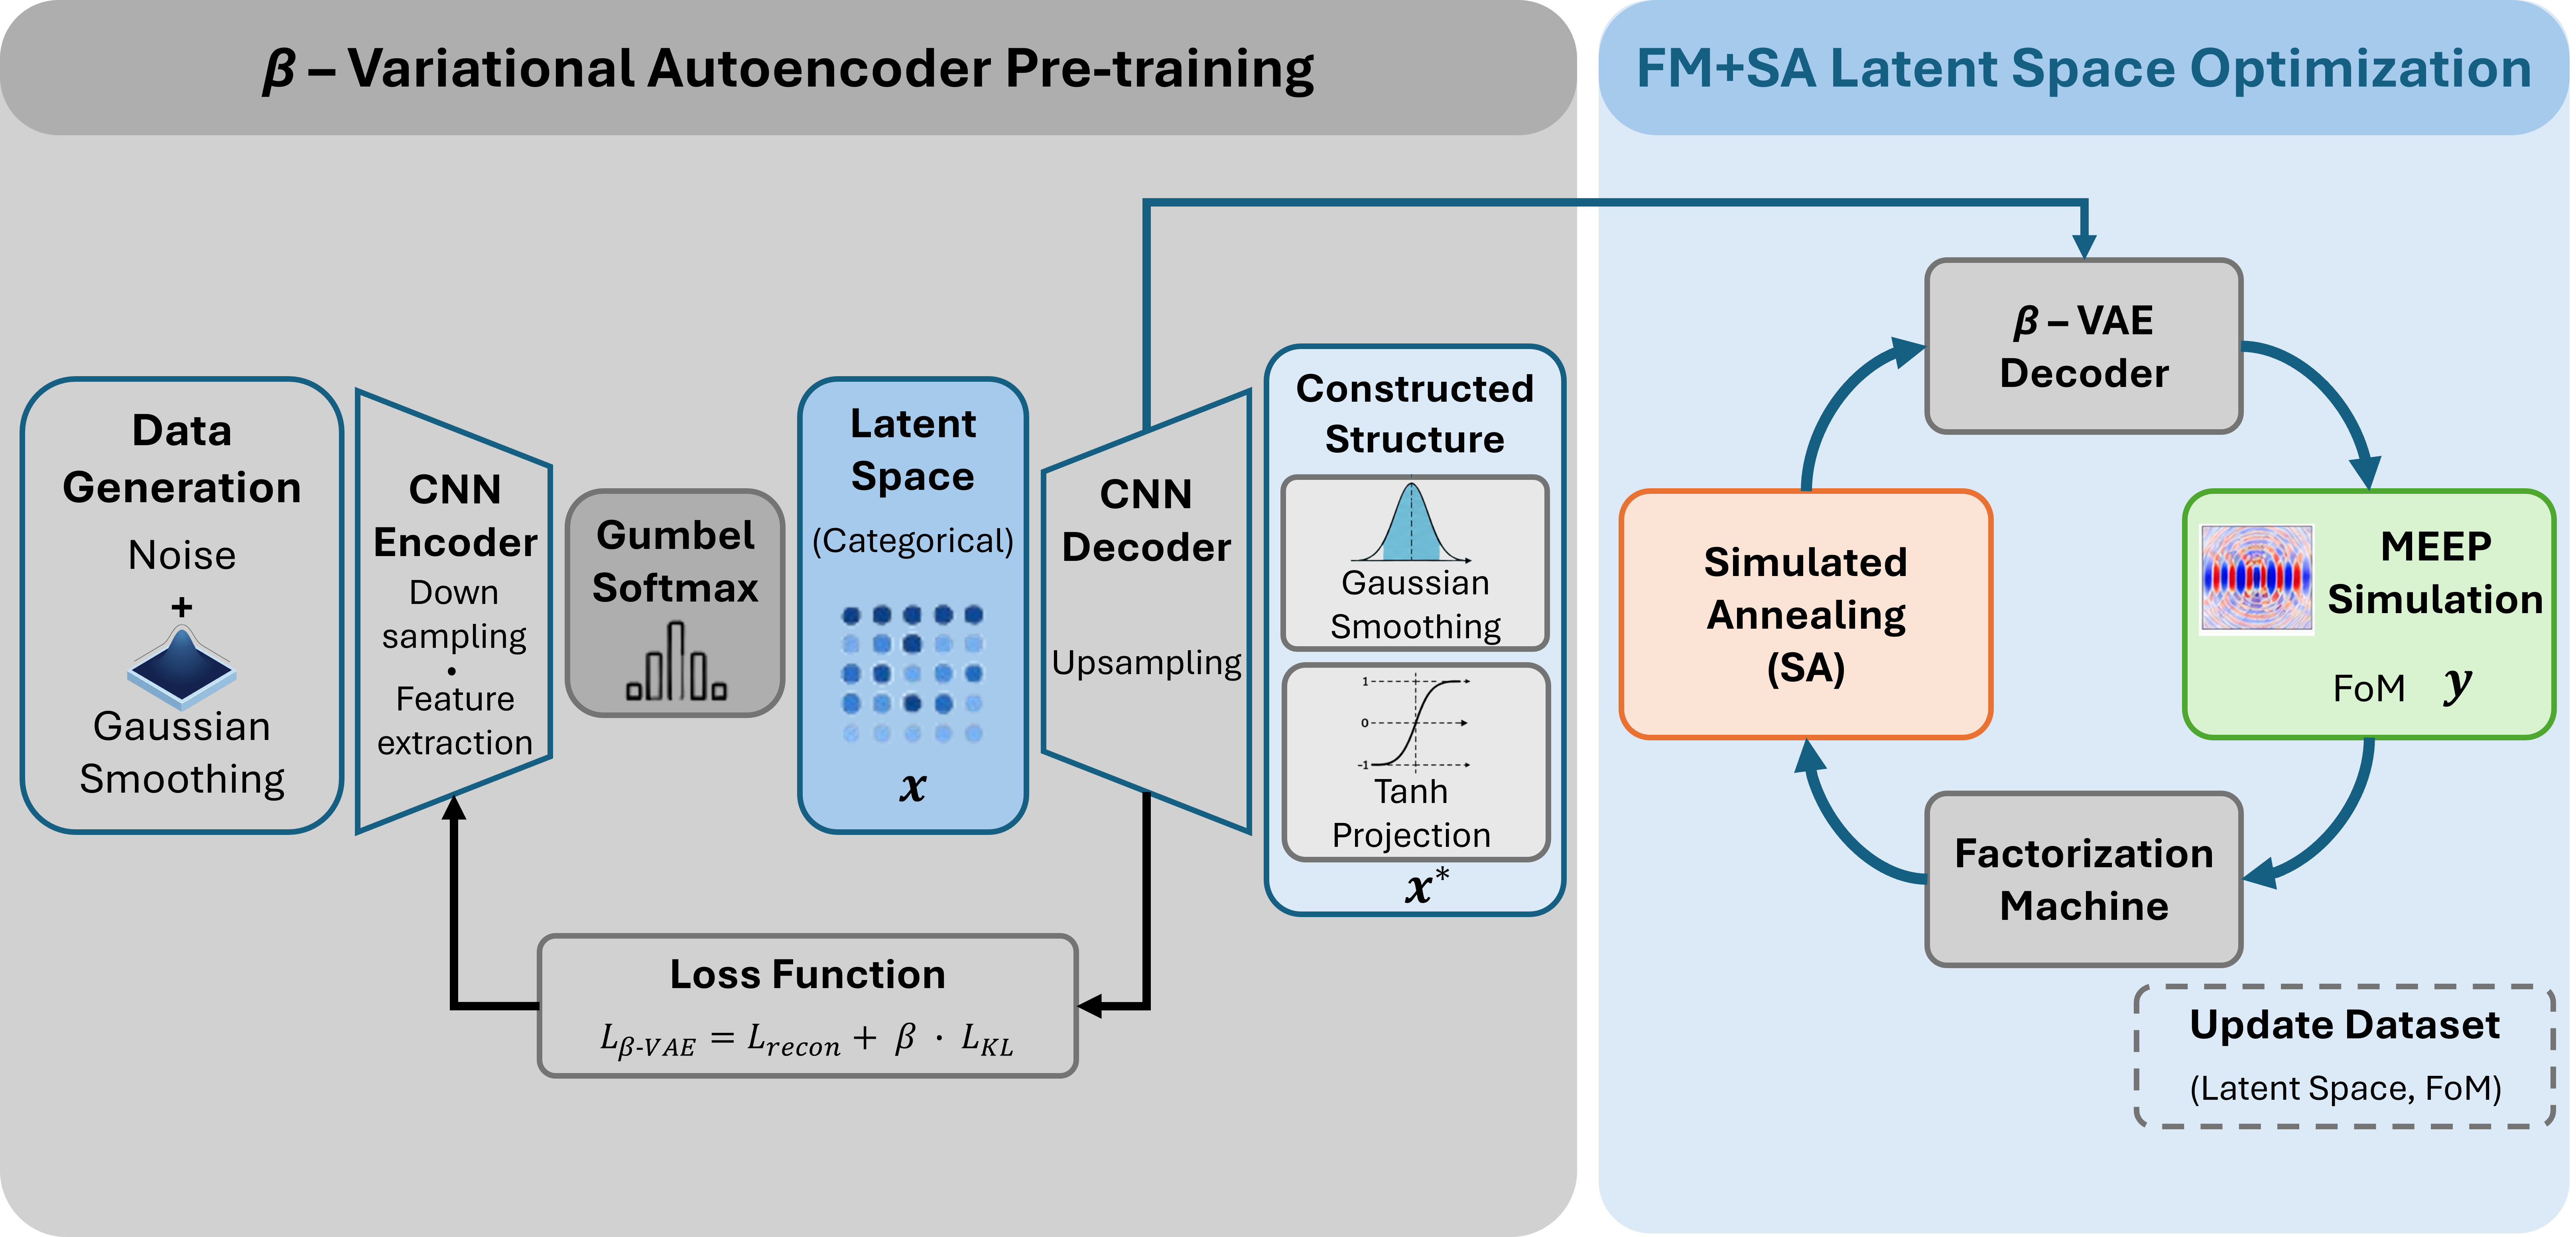
\includegraphics[width=1.0\textwidth]{img/bVAE_flowchart.png}
\caption{$\beta$-VAE編碼策略之整體流程圖。}
\label{fig:bVAE_flowchart}
\end{figure}

模型預訓練的部分，首先建立 $\beta$-VAE 所需的初始訓練資料集部分，程式會以隨機且高維的高斯雜訊作為初始輸入，
並且會經過高斯濾波以及將灰階圖進行二值化處理，以產生具有連續幾何特徵的初始二維結構樣本。
此步驟可以避免訓練資料中出現過多破碎或不連續的孤島結構，使模型能夠學習較為合理的結構分布。

在編碼階段，輸入的初始高解析度二維結構 首先經由卷積神經網路(Convolutional Neural Network, CNN)Encoder 進行特徵擷取。
透過多層卷積與下採樣，輸入的高解析度結構會被壓縮為低維的潛在空間$\boldsymbol{x}$(latent space)。

為了使潛在空間的變數可以直接作為模擬退火的搜尋變數(必須二元值)，會利用 Gumbel-Softmax 方法進行離散化。
Gumbel-Softmax 方法可以將編碼特徵轉換為 $N \times K$ 維的類別型潛在變數，使其可對應為離散的二元值。

在解碼階段，CNN Decoder 接收離散潛在空間，並透過多層的上採樣以及卷積，會逐漸重建為近似原始高解析度的二維結構。
為了降低重建結構中的鋸齒與部分雜訊，Decoder 輸出端同樣也會加入高斯平滑處理，並利用 Tanh 投影函數進行非線性轉換，
使輸出值限制於 $0$ 至 $1$，進而形成近似二值化結構。

在$\beta$-VAE 模型訓練時，損失函數主要是由重建損失$L_{recon}$(Reconstruction Loss)與 Kullback-Leibler 散度$L_{KL}$(KL Divergence)相加組成。
其中，$\beta$ 參數用於調整兩者之間的權重，$\beta$ 理論的部分在第~\ref{ch:bVAE_theory}章有對此部分進行詳細說明。

完成 $\beta$-VAE 的預訓練後，固定 Encoder 與 Decoder 的模型權重，並且
取一部分經過Decoder處理的資料集$\boldsymbol{x}^*$以及其潛在空間$\boldsymbol{x}$用來計算他們的FoM $y$，
當作是我們初始因子分解機的訓練資料。

接著，我們會將這些資料利用因子分解機建立QUBO Matrix，並利用模擬退火採樣器挑選出指定數量的潛在空間較佳解$\boldsymbol{x}_{new}$。
再透過我們訓練好的$\beta$-VAE Decoder重建出高解析度的二維結構$\boldsymbol{x}_{new}^*$作為候選結構，
將得到的候選結構$\boldsymbol{x}_{new}^*$餵給MEEP模擬以驗證其光學性能並計算FoM $y_{new}$。

最後，我們將這一次迭代所得的潛在空間解$\boldsymbol{x}_{new}$與其FoM $y_{new}$，
加入到因子分解機的訓練資料集中，以進行下一次的迭代優化，重複此過程直到達到了最大的迭代次數。

\section{Mode Division Demultiplexer Optimization Results}
此小節我將展示本研究中所提出的利用Encoding策略結合因子分解機與模擬退火應用於模態分波解多工器反向設計的最佳化結果。

首先，我們定義了 Mode Division Demultiplexer 的輸入、輸出通道以及其幾何結構的設計區域，
\begin{figure}[H]
\centering
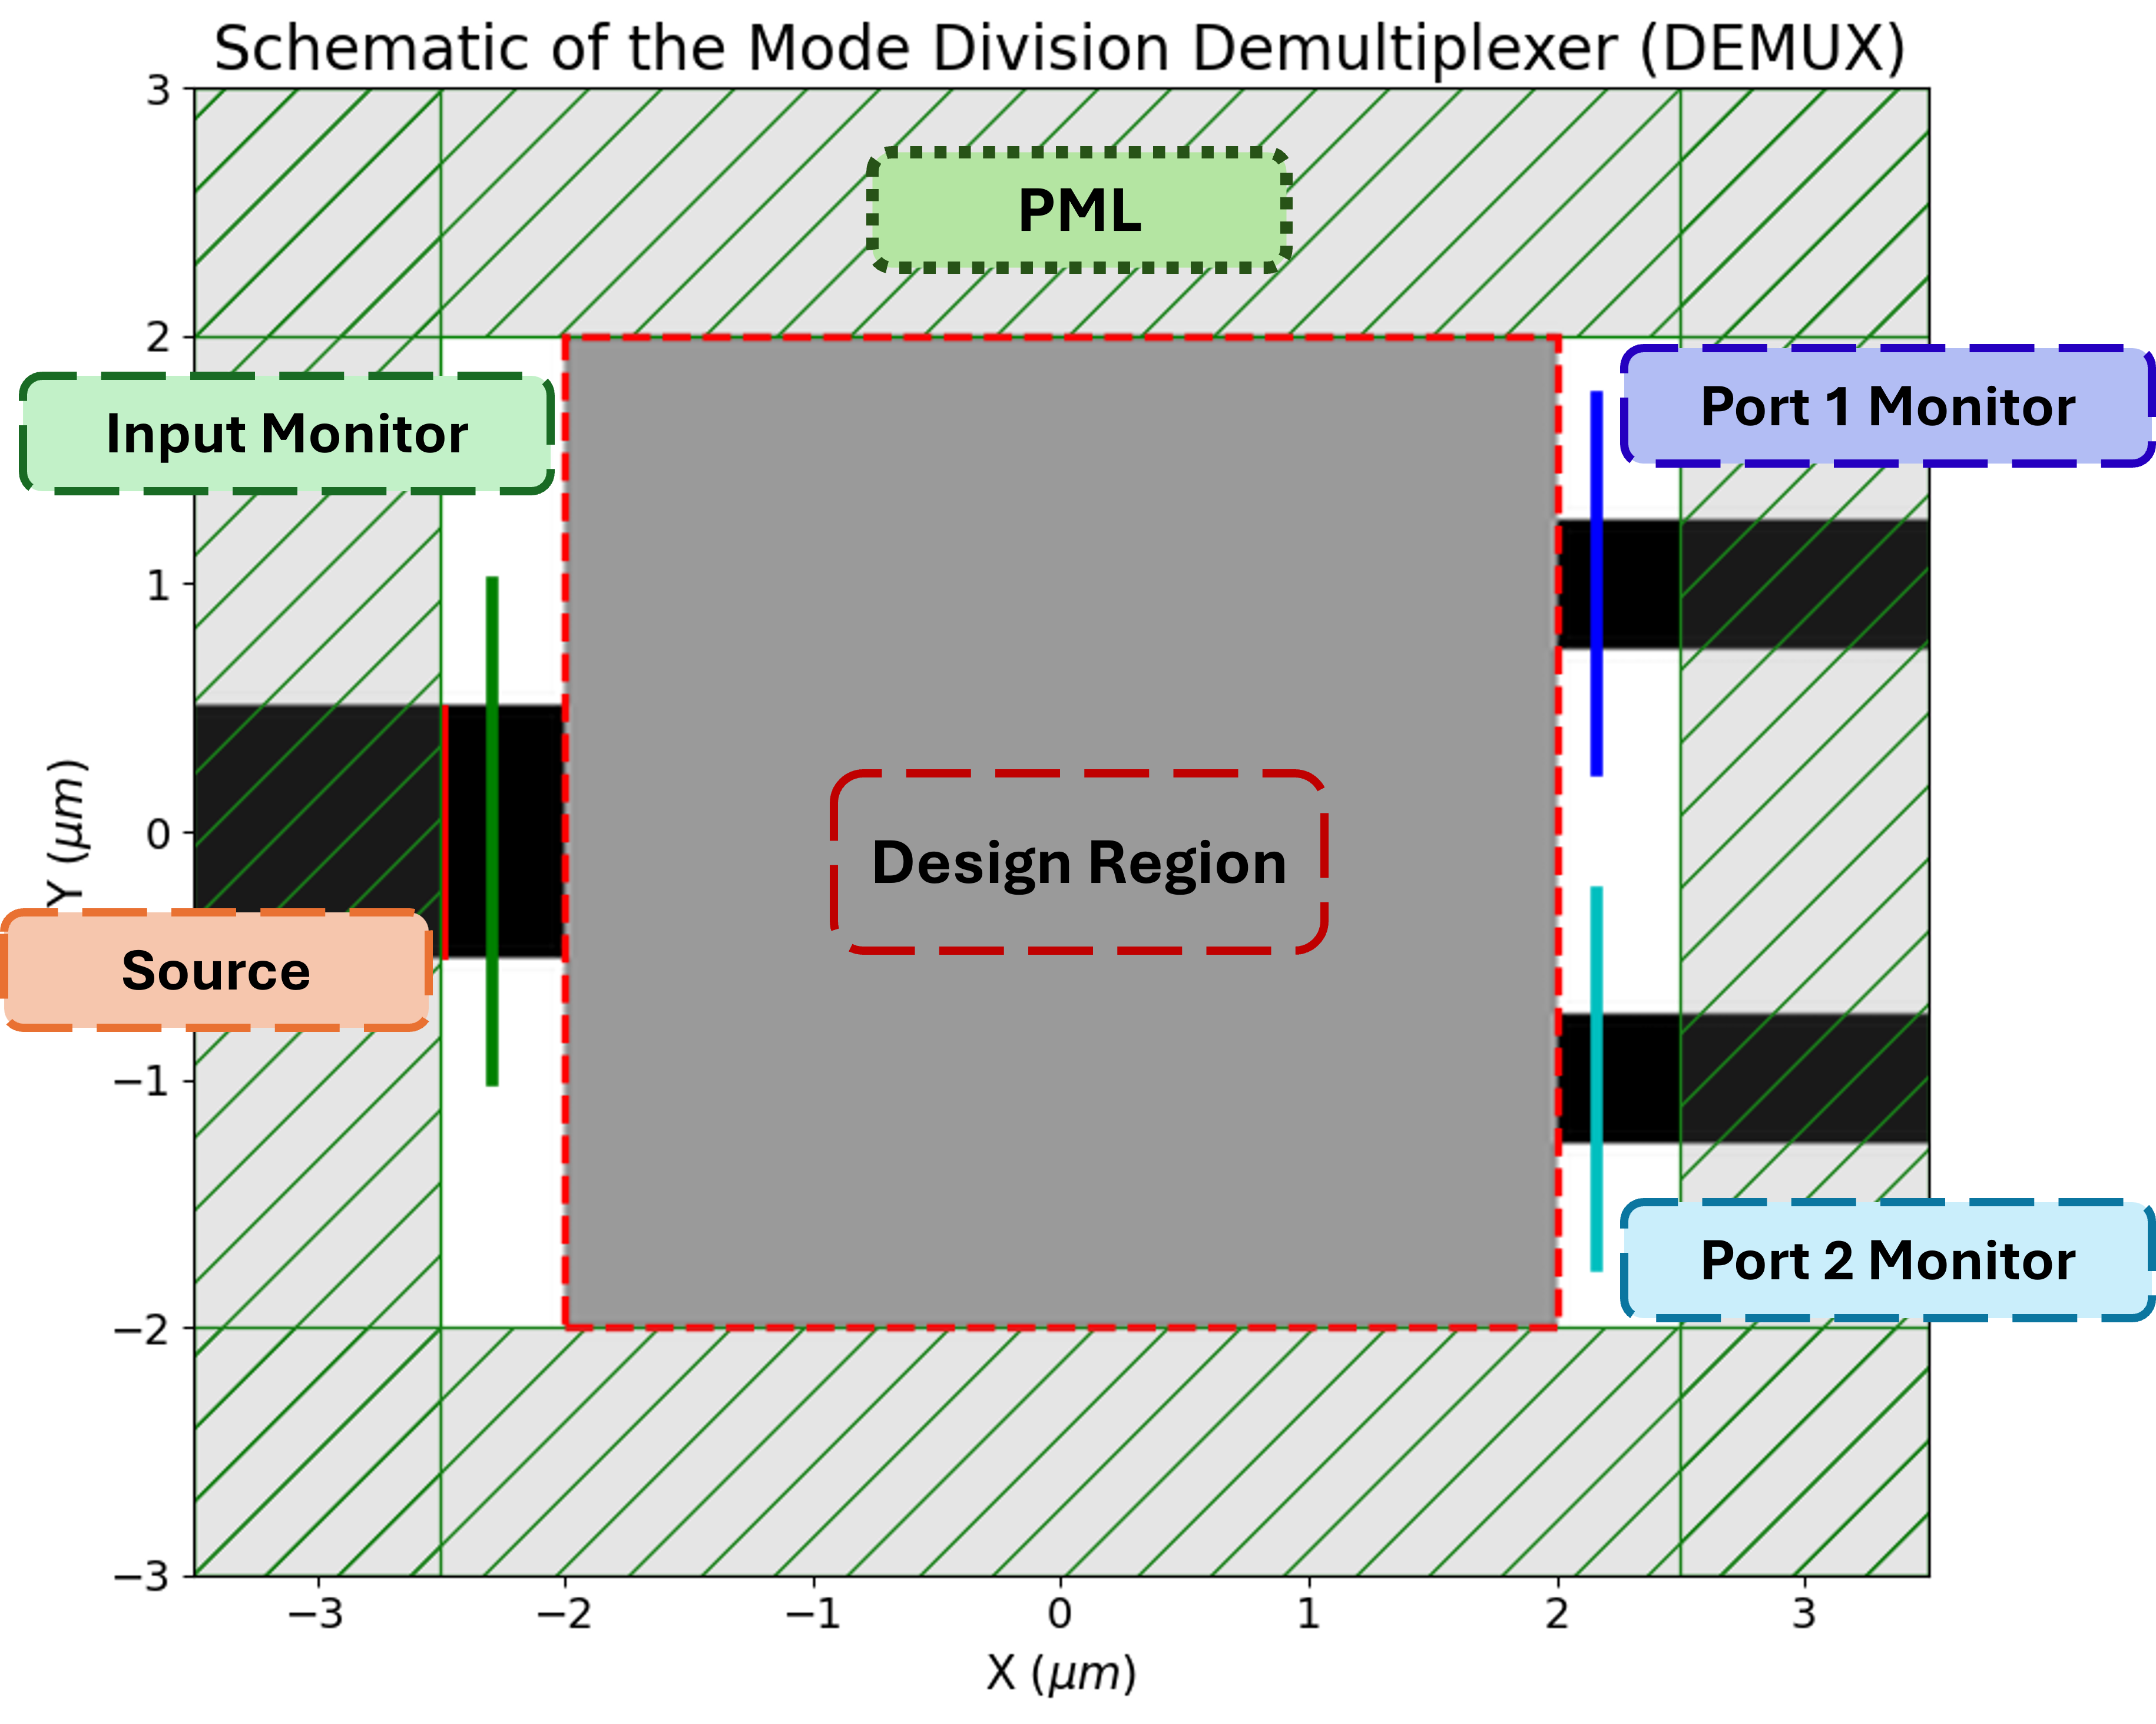
\includegraphics[width=1.0\textwidth]{img/DEMUX_schematic.png}
\caption{Mode Division Demultiplexer 的輸入、輸出通道以及其幾何結構的設計區域。}
\label{fig:DEMUX_schematic}
\end{figure}
如圖~\ref{fig:DEMUX_schematic}所示，中間灰色的部分為演算法決定材料分布的設計區域，
在此模擬中，黑色代表矽(Si)材料，折射率$n_{Si}=3.48$，白色代表二氧化矽(SiO$_2$)材料，折射率$n_{SiO_2}=1.44$。
右側分別為輸出的兩個通道，以及用深藍色與淺藍色標示為輸出通道的模態偵測器;
左側分別為光場輸入通道、利用綠色標示為輸入通道的模態偵測器，以及用紅色標示為光場激發的起點;
在示意圖的最外圍，以深綠色標示出吸收邊界(PML)，用來吸收模擬光場，避免產生反射效應。

接著，光源設定方面，我是使用了MEEP中的EigenModeSource，利用GaussianSource高斯脈衝激發波長為$1550 nm$的光源
，以及分別設定了\text{eig\_band}以及\text{eig\_parity}參數來對應模態數和模態對稱性，
指定要輸入到通道中的 TE$_0$ 與 TE$_1$ 模態。
由於 TE$_0$ 與 TE$_1$ 模態彼此正交，因此於每次 FoM 計算時，分別進行兩次獨立的光學模擬:
第一次在輸入通道激發 TE$_0$ 模態，第二次則激發 TE$_1$ 模態。

本研究之設計目標為將單一輸入通道中的 TE$_0$ 與 TE$_1$ 模態分離並導引至各自對應的輸出通道。
其中，輸入 TE$_0$ 模態時，應使其能量盡可能傳輸至輸出通道1；輸入 TE$_1$ 模態時，則應使其能量傳輸至輸出通道2。
同時，輸出通道1中的 TE$_1$ 模態能量應盡可能降低，以抑制模態串擾(crosstalk)。\\
因此，本研究定義下列 Figure of Merit(FoM)作為 DEMUX 結構之最佳化目標:
\begin{align}
FOM = \left[ T_{0,1} (1 - T_{0,2}) \times T_{1,2} (1 - T_{1,1}) \right]
\label{eq:DEMUX_FoM}
\end{align}
其中，
\begin{itemize}
    \item $T_{0,1}$ 為輸入 TE$_0$ 模態時，其能量傳輸至輸出通道1的穿透率
    \item $T_{0,2}$ 為輸入 TE$_0$ 模態時，其能量傳輸至輸出通道2的穿透率
    \item $T_{1,1}$ 為輸入 TE$_1$ 模態時，其能量傳輸至輸出通道1的穿透率
    \item $T_{1,2}$ 為輸入 TE$_1$ 模態時，其能量傳輸至輸出通道2的穿透率
\end{itemize}
首先，$T_{0,1}(1 - T_{0,2})$項與$T_{1,2}(1 - T_{1,1})$項分別代表了各別模態內部的取捨與目標，
用來提升主要目標穿透率的同時，抑制模態串擾。其次，此公式當設計結果越好，其數值越接近$1$。

\subsection{DEMUX design - parameter 1}
\label{ch:DEMUX_design1}
最一開始設計模態分波多工器的設計區域為$6.5 \times 6.5\ \mu m^2$，並且採用$8 \times 8$ 的網格進行劃分，在這個階段目的主要用於驗證
高斯上採樣(Gaussian Upsampling)方法結合FMSA的初步可行性，並且在多模態波導的部分設定寬度為$1.8\mu m$，可支持TE$_0$與TE$_1$的傳輸;
單模波導寬度設定為$0.5\mu m$，只允許TE$_0$的傳輸。

在訓練參數上，用來訓練因子分解機的初始隨機資料量為$1000$筆，隨後進行$100$次的迭代，並且每次迭代會利用模擬退火隨機採樣$30$個候選解，因此總資料量為$4000$筆。

最終得到品質因數FOM為:
\begin{align}
FOM = 0.2196
\label{eq:DEMUX_FoM_Design1}
\end{align}
而最終模擬結果為:(光場分布結果如圖~\ref{fig:DEMUX_design1_TE0mode}與圖~\ref{fig:DEMUX_design1_TE1mode}所示)
\begin{itemize}
    \item $T_{0,1}$ 穿透率 : 62.66\% ($-2.03$ dB)
    \item $T_{1,2}$ 穿透率 : 41.3\% ($-3.839$ dB)
    \item $T_{0,2}$ 模態串擾 : 3\% ($-15.22$ dB)
    \item $T_{1,1}$ 模態串擾 : 12.6\% ($-8.99$ dB)
\end{itemize}

\begin{figure}[H]
     \centering
     \begin{subfigure}[]{0.8\textwidth}
         \centering
         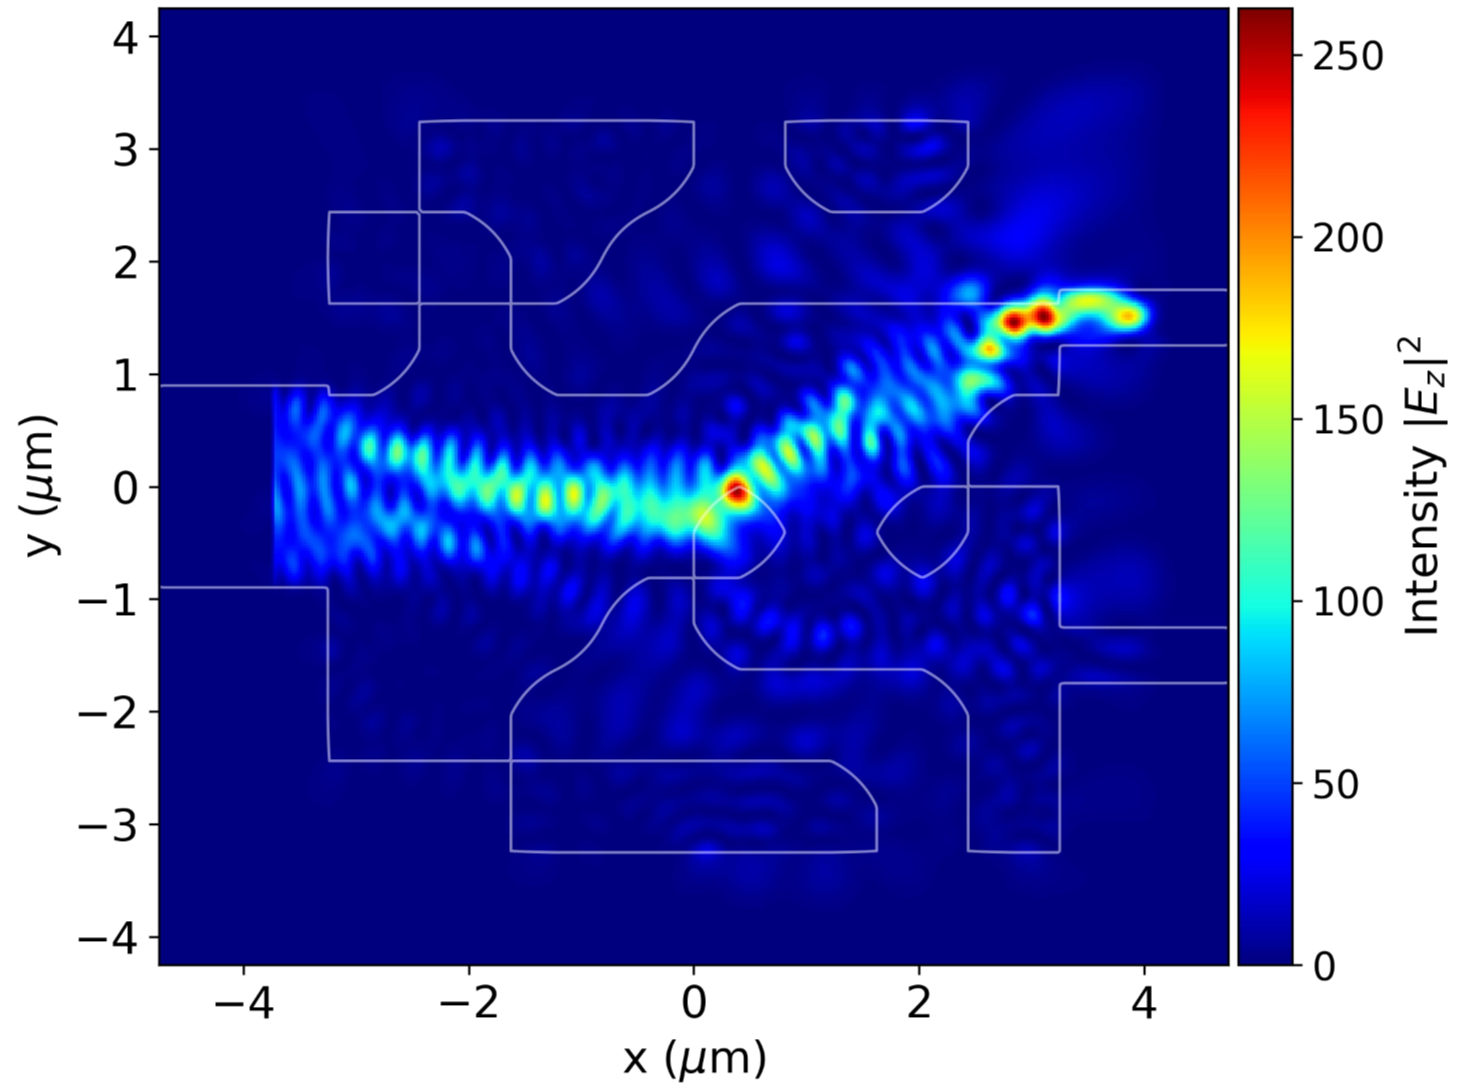
\includegraphics[width=\textwidth]{img/DEMUX/DEMUX-design1/replot_output/Design1_TE0.png}
         \caption{DEMUX Design 1 TE$_0$ mode DFT Distribution.}
         \label{fig:DEMUX_design1_TE0mode}
     \end{subfigure}
     
     \begin{subfigure}[]{0.8\textwidth}
         \centering
         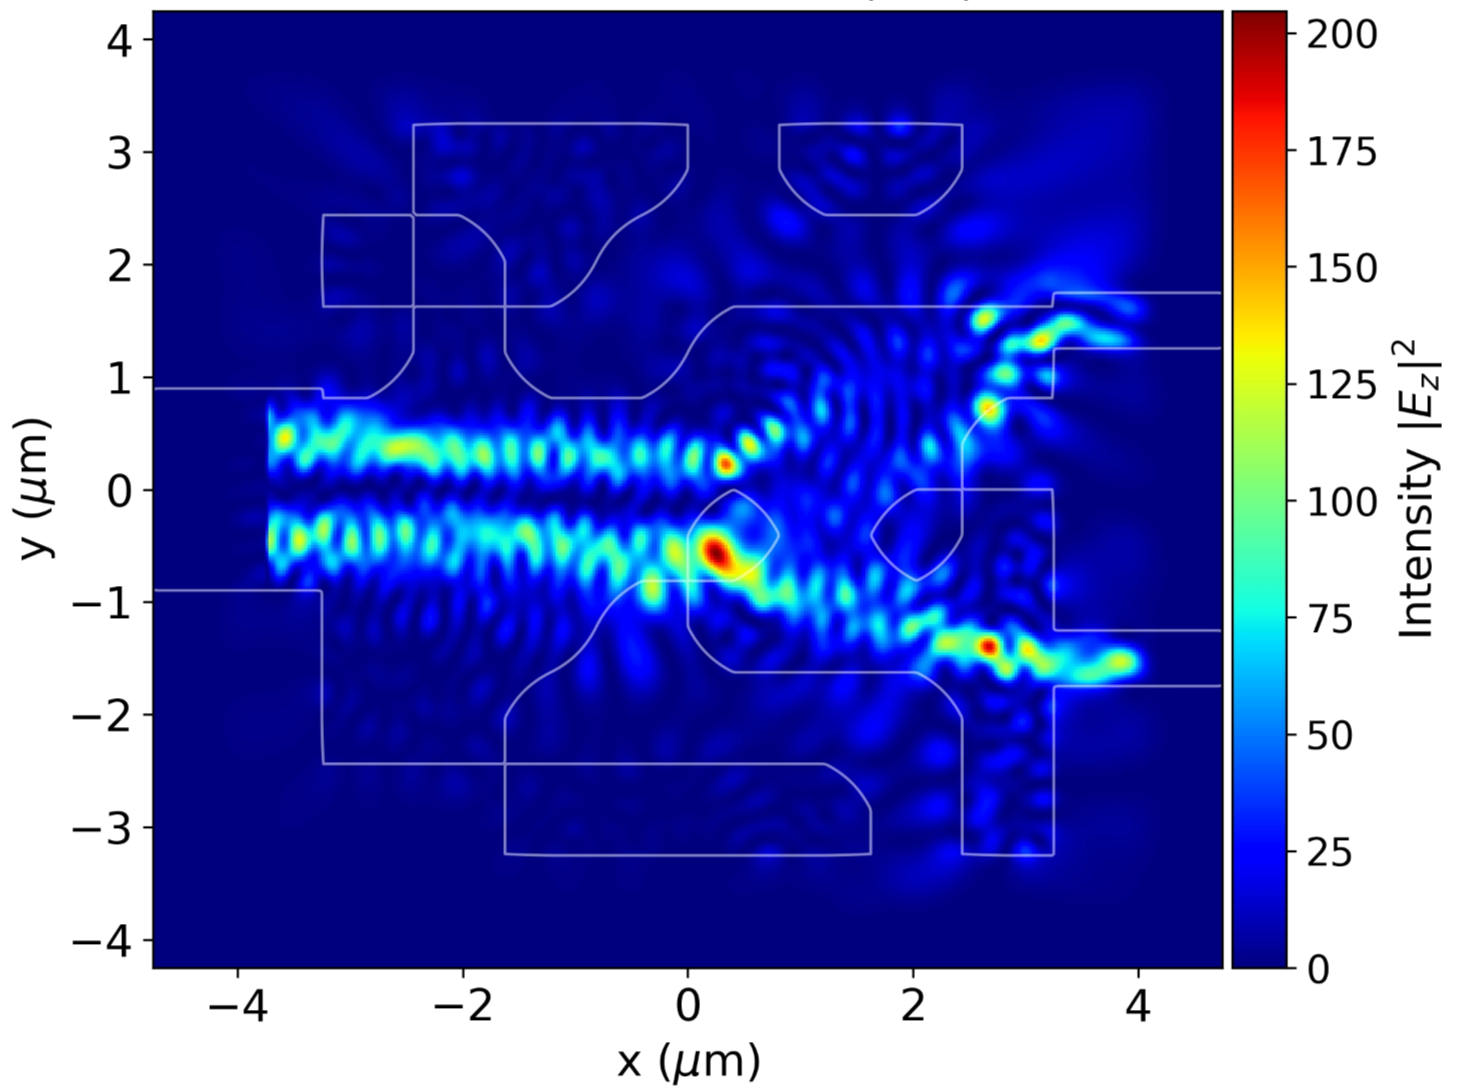
\includegraphics[width=\textwidth]{img/DEMUX/DEMUX-design1/replot_output/Design1_TE1.png}
         \caption{DEMUX Design 1 TE$_1$ mode DFT Distribution.}
         \label{fig:DEMUX_design1_TE1mode}
     \end{subfigure}
     \caption{DEMUX Design 1 DFT Field Distribution.}
     \label{fig:DEMUX_design1_SimulationResult}
\end{figure}

\subsection{DEMUX design - parameter 2}
\label{ch:DEMUX_design2}
接著，為解決光場在輸入與輸出端口容易發散的問題，我嘗試在輸入輸出端口連接設計區域的部分添加填充方塊結構(Padding)，並將其視為固定結構，
不參與最佳化搜尋，以此來引導光場傳輸到指定的輸出端口。
其餘的設計結構設定與訓練參數皆與上一個實驗(第~\ref{ch:DEMUX_design1})相同。

最終品質因數FOM提升至:
\begin{align}
FOM = 0.2728
\label{eq:DEMUX_FoM_Design2}
\end{align}
而最終模擬結果為:
\begin{itemize}
    \item $T_{0,1}$ 穿透率 : 54.63\% ($-2.625$ dB)
    \item $T_{1,2}$ 穿透率 : 54.73\% ($-2.617$ dB)
    \item $T_{0,2}$ 模態串擾 : 6.27\% ($-12.02$ dB)
    \item $T_{1,1}$ 模態串擾 : 2.36\% ($-16.26$ dB)
\end{itemize}
由最終光場分布結果(如圖~\ref{fig:DEMUX_design2_TE0mode}與圖~\ref{fig:DEMUX_design2_TE1mode}所示)可以發現，在加入固定填充方塊結構後，
光場更能有效的被引導至對應的輸出端口，因此提升了品質因數FOM。
\begin{figure}[H]
     \centering
     \begin{subfigure}[]{0.8\textwidth}
         \centering
         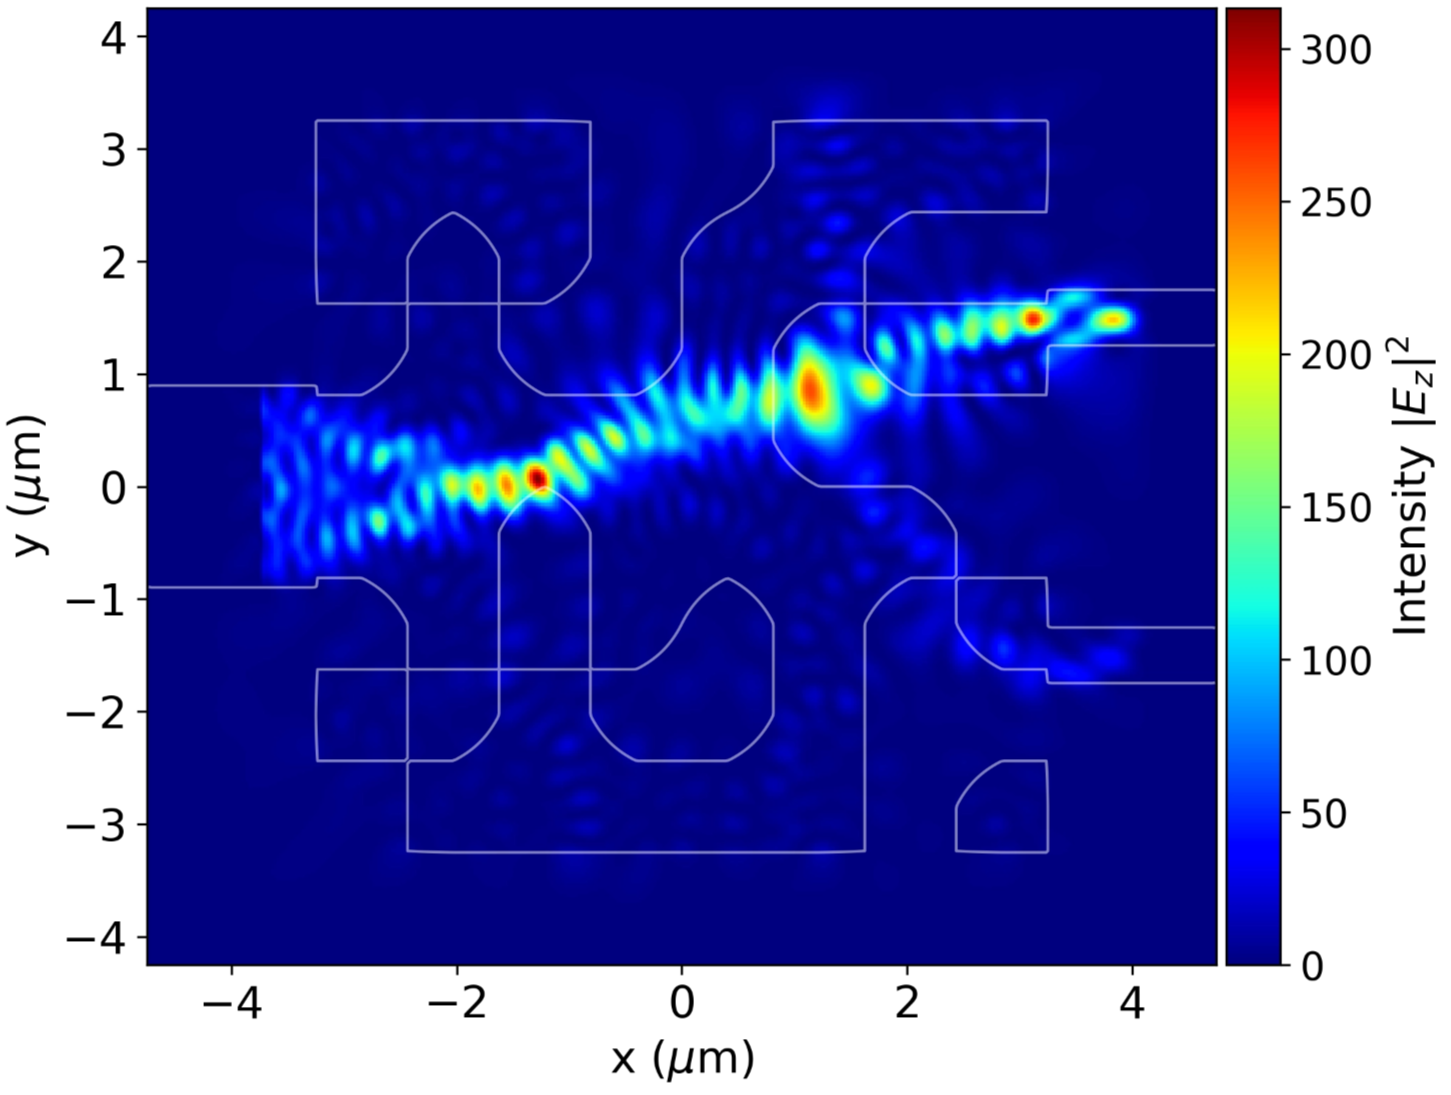
\includegraphics[width=\textwidth]{img/DEMUX/DEMUX-design2/design2_TE0.png}
         \caption{DEMUX Design 2 TE$_0$ mode DFT Distribution.}
         \label{fig:DEMUX_design2_TE0mode}
     \end{subfigure}
     
     \begin{subfigure}[]{0.8\textwidth}
         \centering
         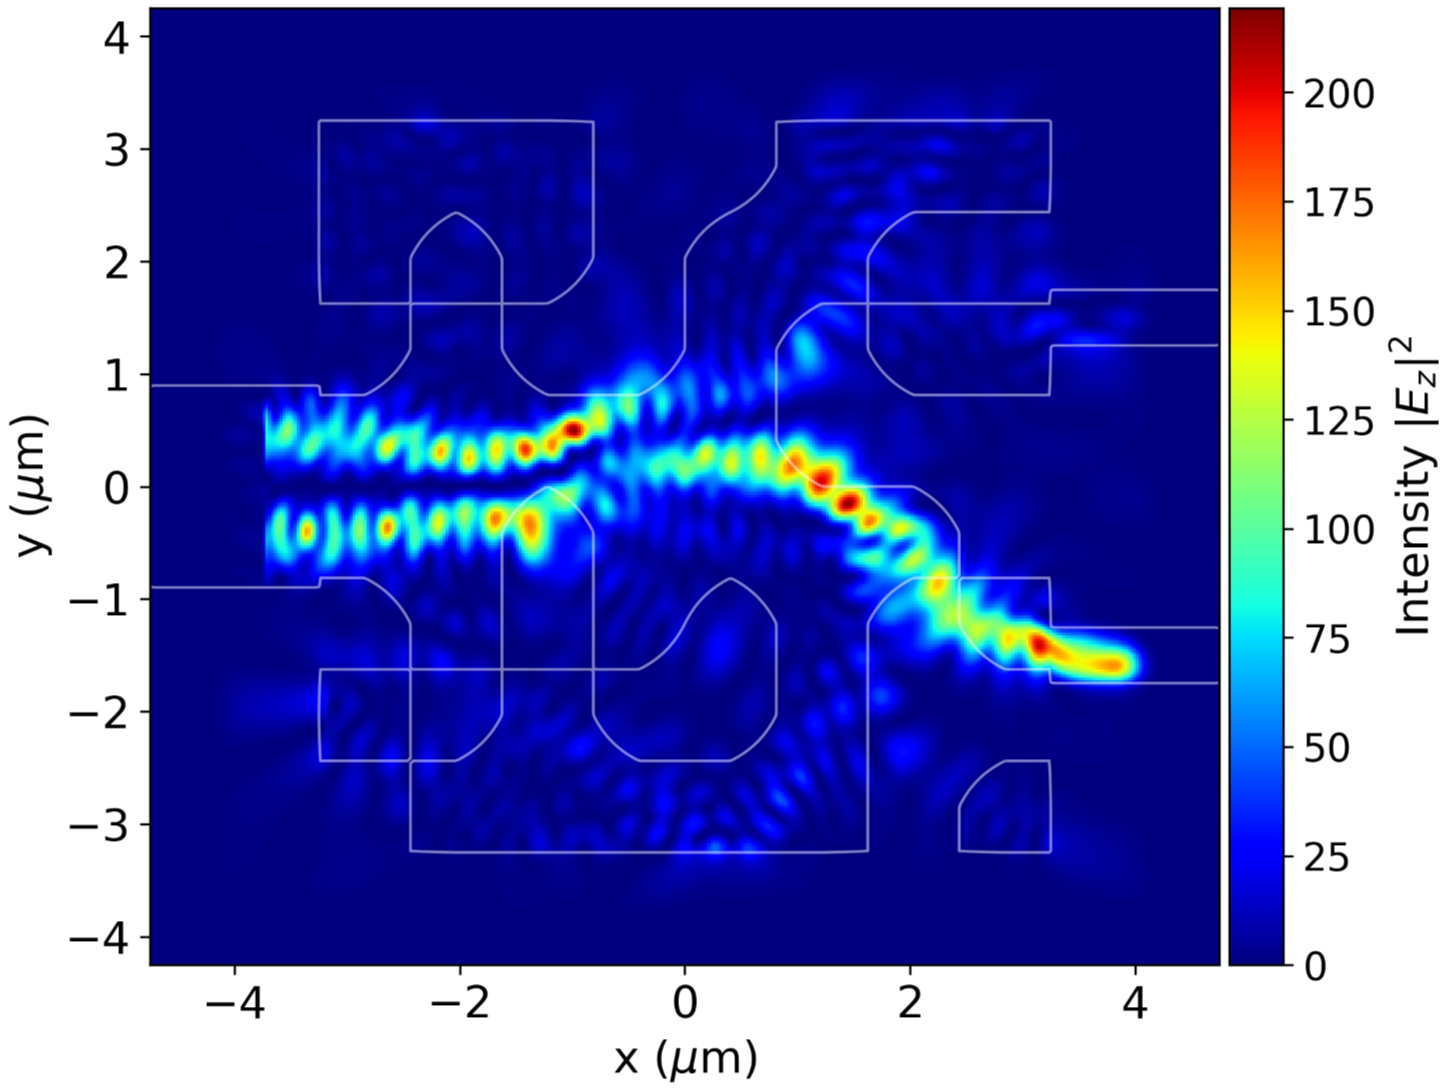
\includegraphics[width=\textwidth]{img/DEMUX/DEMUX-design2/design2_TE1.png}
         \caption{DEMUX Design 2 TE$_1$ mode DFT Distribution.}
         \label{fig:DEMUX_design2_TE1mode}
     \end{subfigure}
     \caption{DEMUX Design 2 DFT Field Distribution.}
     \label{fig:DEMUX_design2_SimulationResult}
\end{figure}

\subsection{DEMUX design - parameter 3}
為了減少光場在非線性轉換過程中的傳播時間與距離，我們將設計區域縮小為$4.0 \times 4.0 \mu m^2$，並且將網格劃分設定為$10 \times 10$，來增加設計變數的維度，
使其對於結構設計有更多的自由度，並且將多模態波導寬度設定為$1.0\mu m$。其餘的結構設定與訓練參數皆與上一個實驗(第~\ref{ch:DEMUX_design2}節)相同。

最終品質因數FOM為:
\begin{align}
FOM = 0.2177
\label{eq:DEMUX_FoM_Design3}
\end{align}
而最終模擬結果為:
\begin{itemize}
    \item $T_{0,1}$ 穿透率 : 58.36\% ($-2.34$ dB)
    \item $T_{1,2}$ 穿透率 : 38.81\% ($-4.11$ dB)
    \item $T_{0,2}$ 模態串擾 : 1.60\% ($-17.97$ dB)
    \item $T_{1,1}$ 模態串擾 : 2.32\% ($-16.35$ dB)
\end{itemize}
由最終光場分布結果(如圖~\ref{fig:DEMUX_design3_TE0mode}與圖~\ref{fig:DEMUX_design3_TE1mode}所示)可以發現，即使將設計區域縮小，元件依然保持了穩定的分波功能，
但能量傳輸至目標端口的效率略為下降，可能的原因為:\\
\noindent 1.設計區域縮小限制了光場調變的有效傳播距離，無法有效輸出可以被波導接收的散射損耗，導致轉換效率下降。\\
\noindent 2.雖然將網格劃分設定為$10 \times 10$ 增加了設計的自由度，但也增加了設計複雜度，當演算法在控制光場的破壞性與建設性干涉時，會導致部分的雜散光無法被限制，
進而導致穿透率下降。\\
\noindent 3.從模態串擾的角度來看，表示在結構縮小之後還是可以保持相位匹配的條件來維持模態分波的品質，因此可以推測效率下降可能是因為設計區域縮小而導致的邊緣散射，
而不是模態間的能量耦合錯誤。
\begin{figure}[H]
     \centering
     \begin{subfigure}[]{0.8\textwidth}
         \centering
         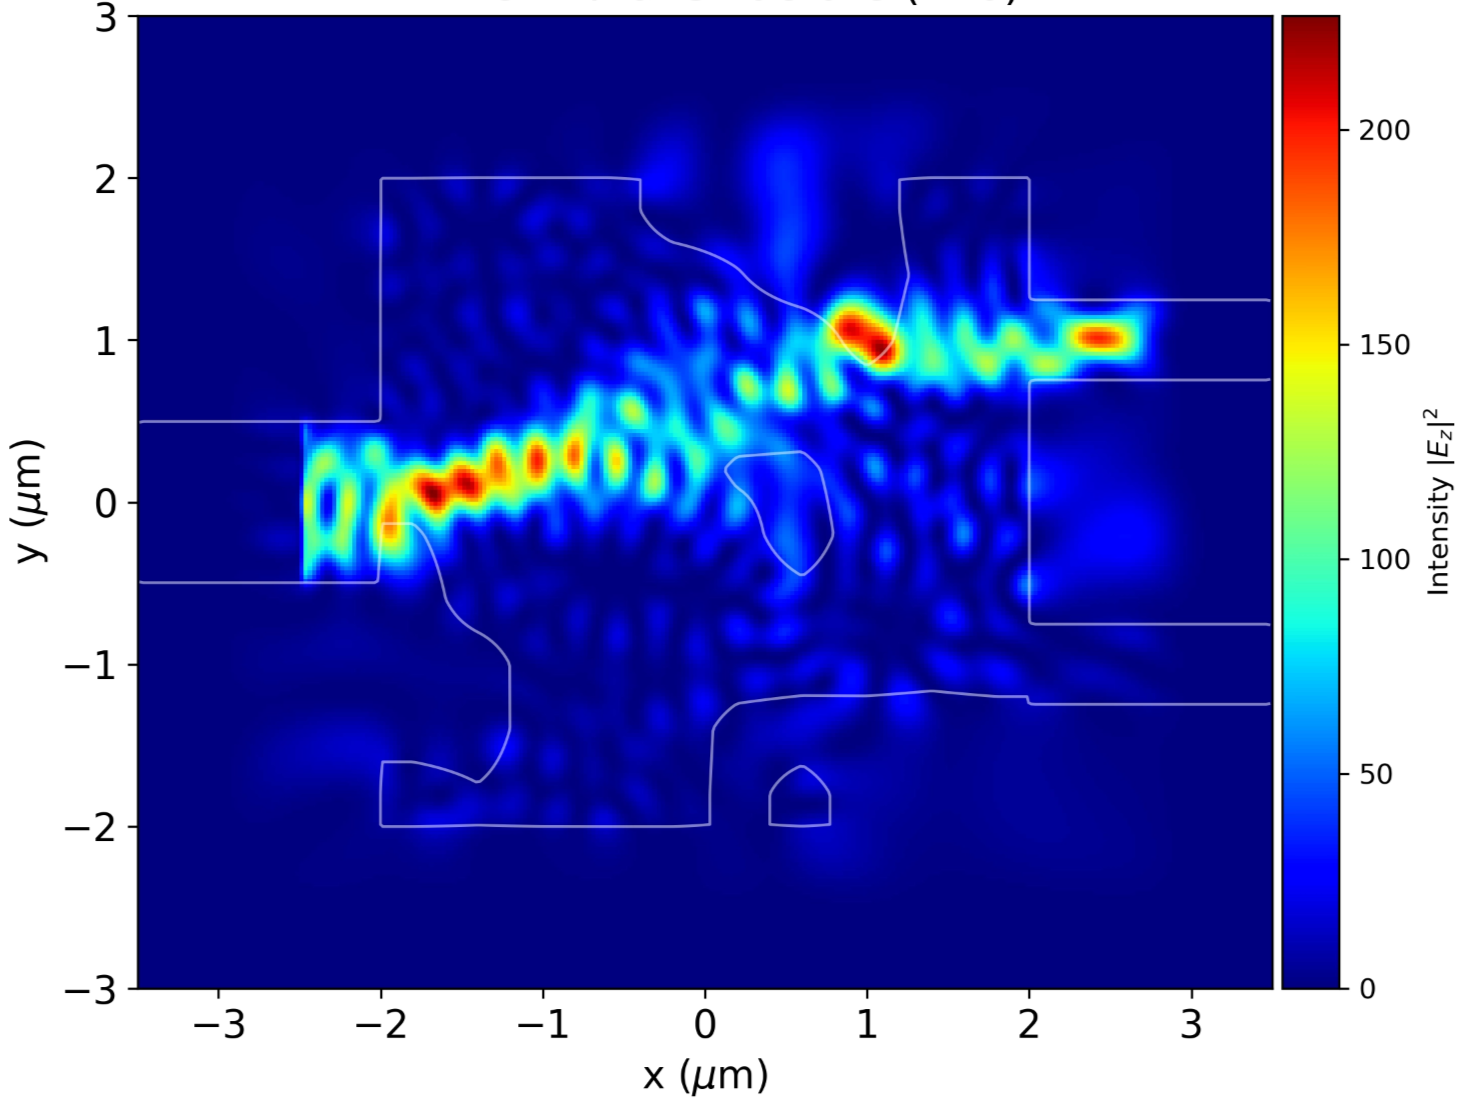
\includegraphics[width=\textwidth]{img/DEMUX/DEMUX-design3/design3_TE0.png}
         \caption{DEMUX Design 3 TE$_0$ mode DFT Distribution.}
         \label{fig:DEMUX_design3_TE0mode}
     \end{subfigure}
     
     \begin{subfigure}[]{0.8\textwidth}
         \centering
         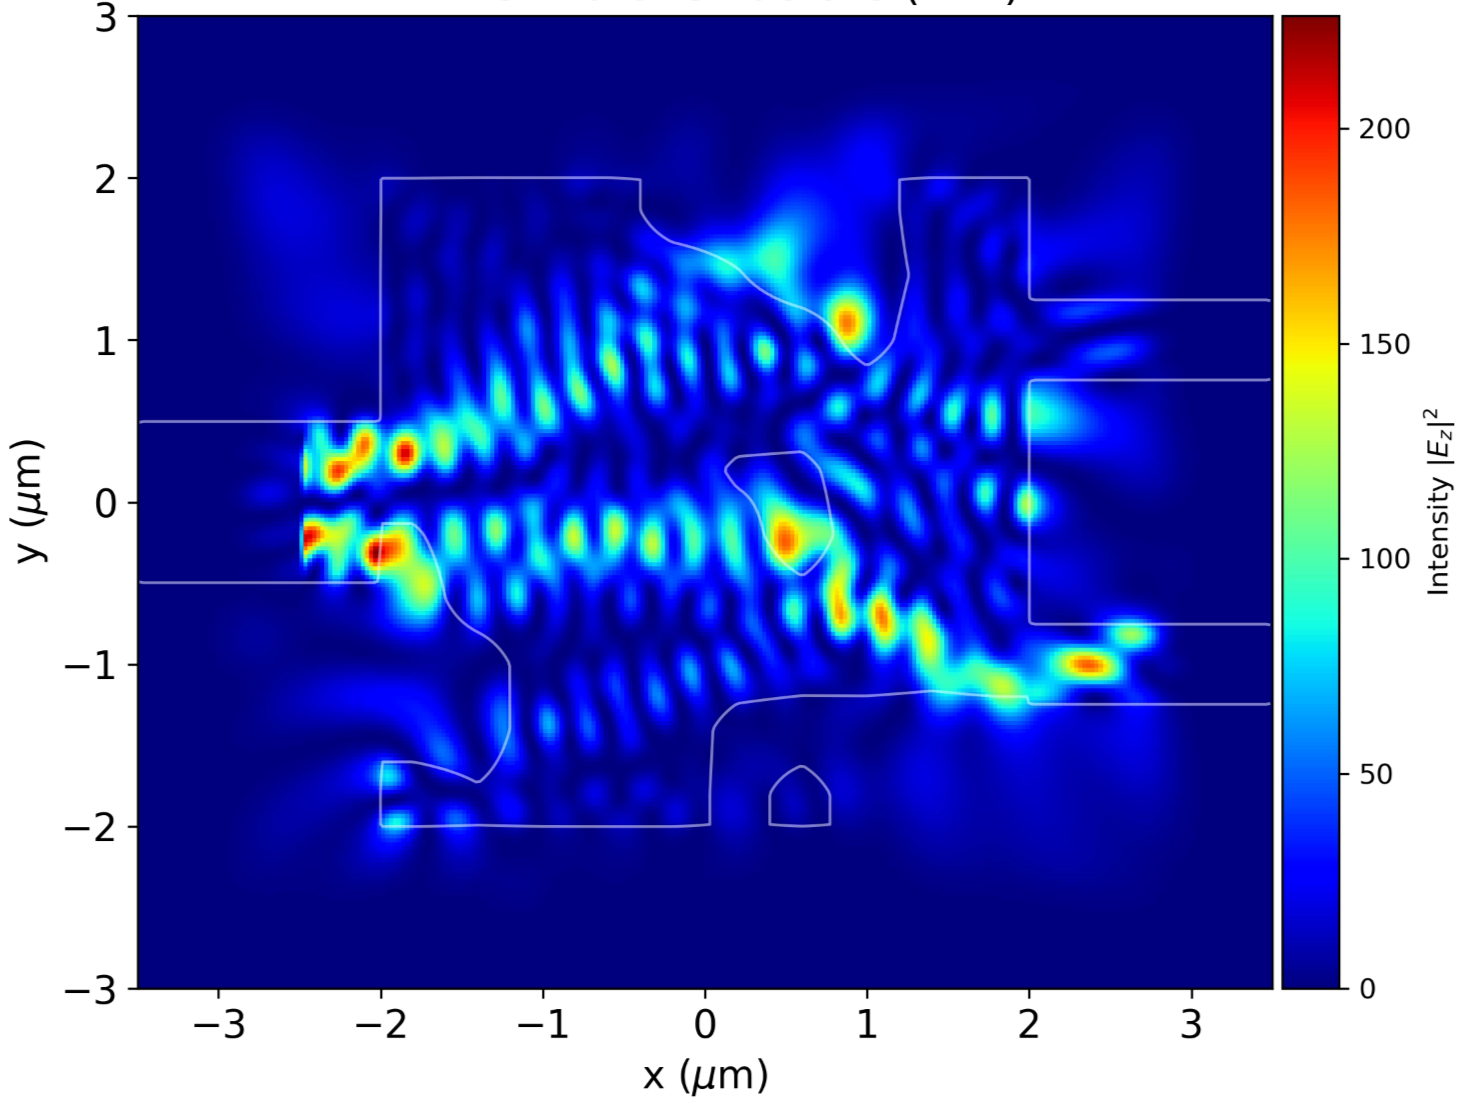
\includegraphics[width=\textwidth]{img/DEMUX/DEMUX-design3/design3_TE1.png}
         \caption{DEMUX Design 3 TE$_1$ mode DFT Distribution.}
         \label{fig:DEMUX_design3_TE1mode}
     \end{subfigure}
     \caption{DEMUX Design 3 DFT Field Distribution.}
     \label{fig:DEMUX_design3_SimulationResult}
\end{figure}

\subsection{DEMUX design - parameter 4}
接著，我們在設計區域相同($4.0 \times 4.0 \mu m^2$)的情況下，將網格劃分設定提高為$16 \times 16$，透過增加設計變數的維度，來提供演算法更高的設計自由度。
其餘的設計結構設定與訓練參數皆與前面的實驗(第~\ref{ch:DEMUX_design2}節)相同。

最終品質因數FOM為:
\begin{align}
FOM = 0.1247
\label{eq:DEMUX_FoM_Design4}
\end{align}
而最終模擬結果為:
\begin{itemize}
    \item $T_{0,1}$ 穿透率 : 46.26\% ($-3.35$ dB)
    \item $T_{1,2}$ 穿透率 : 27.86\% ($-5.55$ dB)
    \item $T_{0,2}$ 模態串擾 : 3.13\% ($-15.05$ dB)
    \item $T_{1,1}$ 模態串擾 : 0.06\% ($-32.33$ dB)
\end{itemize}

由最終光場分布結果(如圖~\ref{fig:DEMUX_design4_TE0mode}與圖~\ref{fig:DEMUX_design4_TE1mode}所示)可以發現$16 \times 16$的網格劃分設定設計出的結構雖然可以帶給我們更多的結構變形與不規則輪廓，
但對於傳統的模態分波多工器來說，要在極小距離內實現穩定的模態分流，結構更需要的或許是更精細且分布均勻的微小單元，用來提供部分區域的有效折射率調變來進行相位匹配的條件，
而非過度追求設計自由度所帶來的不規則結構。
\begin{figure}[H]
     \centering
     \begin{subfigure}[]{0.8\textwidth}
         \centering
         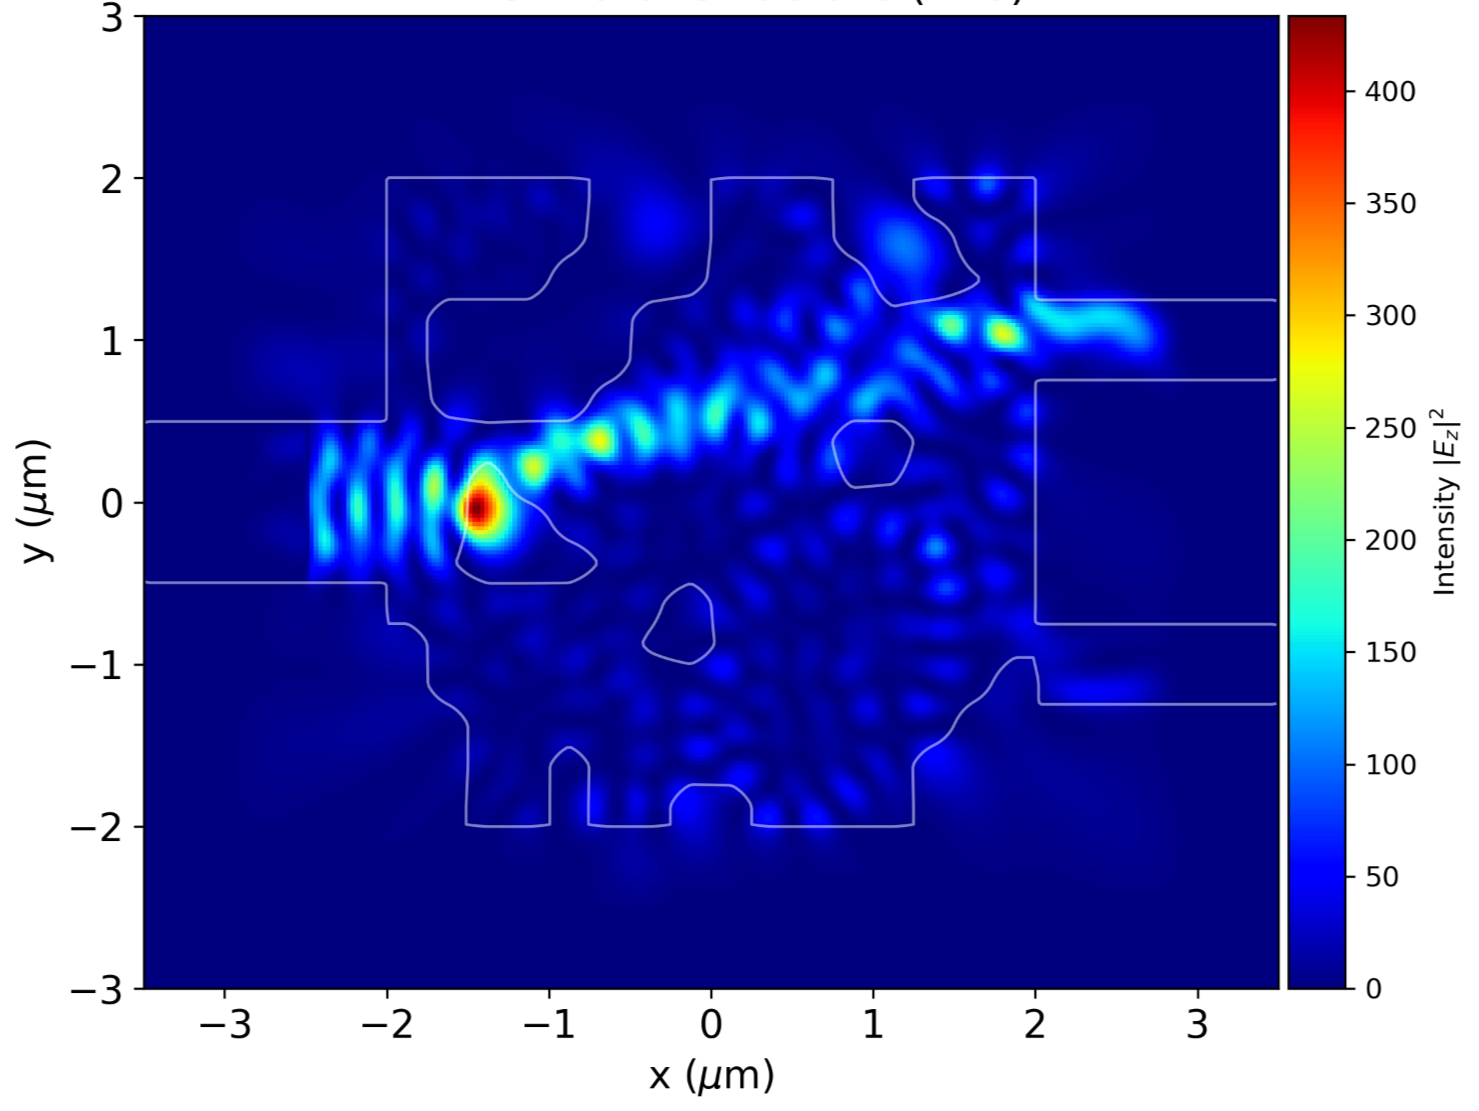
\includegraphics[width=\textwidth]{img/DEMUX/DEMUX-design4/design4_TE0.png}
         \caption{DEMUX Design 4 TE$_0$ mode DFT Distribution.}
         \label{fig:DEMUX_design4_TE0mode}
     \end{subfigure}
     
     \begin{subfigure}[]{0.8\textwidth}
         \centering
         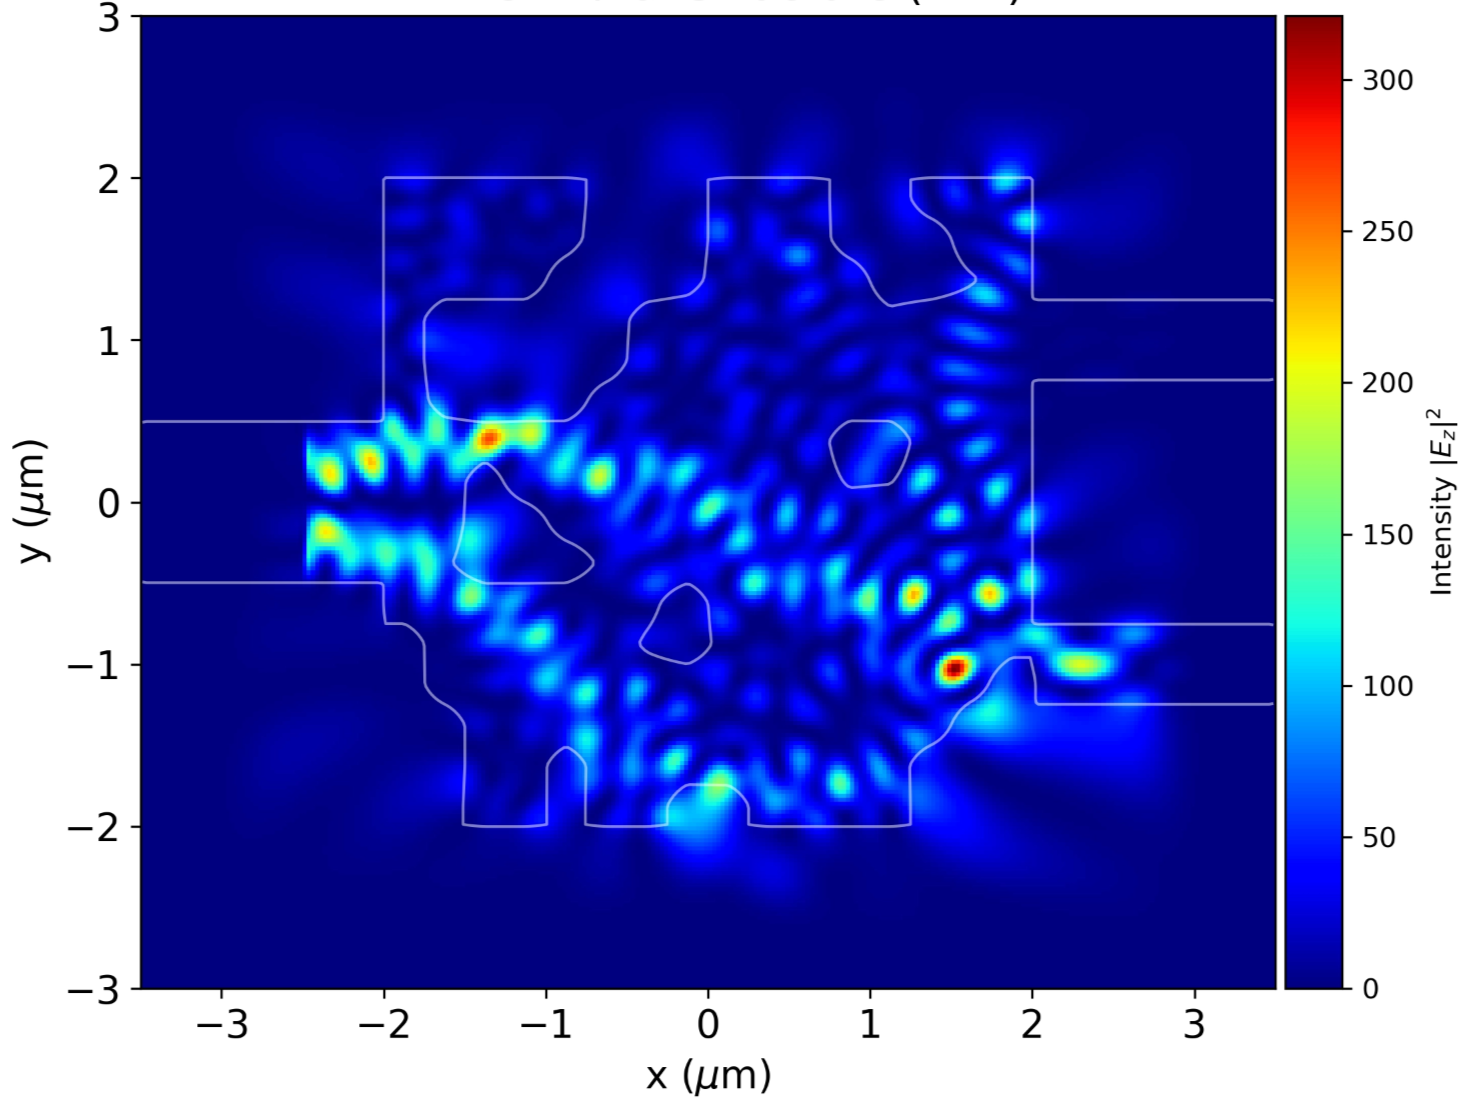
\includegraphics[width=\textwidth]{img/DEMUX/DEMUX-design4/design4_TE1.png}
         \caption{DEMUX Design 4 TE$_1$ mode DFT Distribution.}
         \label{fig:DEMUX_design4_TE1mode}
     \end{subfigure}
     \caption{DEMUX Design 4 DFT Field Distribution.}
     \label{fig:DEMUX_design4_SimulationResult}
\end{figure}

可以從圖~\ref{fig:DEMUX_design4_bestfom_vs_iter}中發現，演算法在大約第10次迭代後，FoM就不再增加，可以推測演算法在第10次迭代陷入局部最佳解，這導致最終的結構不但無法有效利用高自由度所帶來的優勢，
反而因為缺乏大範圍的結構協調性，使 $T_{0,1}$ 穿透率下降為 46.26\%，FoM 降至 0.1247。
\begin{figure}[H]
\centering
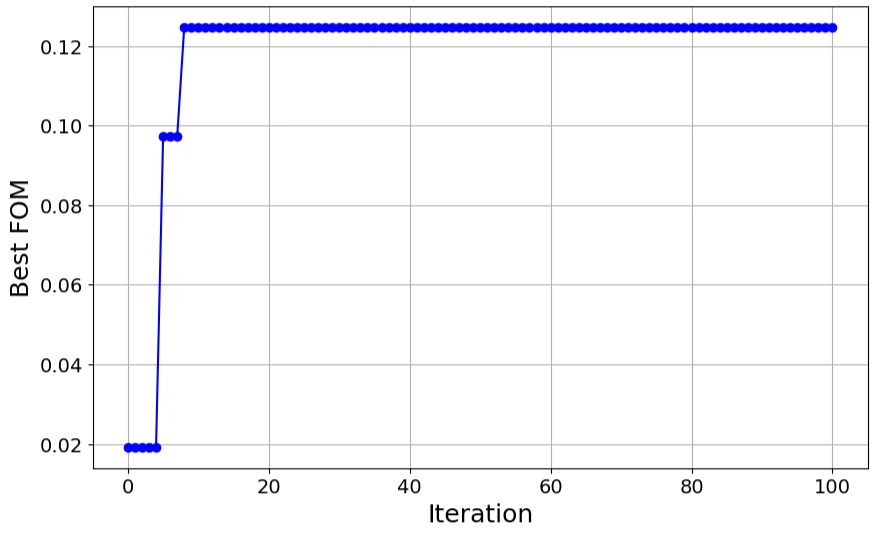
\includegraphics[width=0.8\textwidth]{img/DEMUX/DEMUX-design4/bestfom_vs_iter.png}
\caption{Best FoM vs Iteration}
\label{fig:DEMUX_design4_bestfom_vs_iter}
\end{figure}

\section{Bend Waveguide Optimization Results}
此小節我將展示本研究中所提出的三種Encoding策略結合因子分解機與模擬退火應用於彎曲波導(Bend Waveguide)反向設計的最佳化結果。

首先，我們定義了彎曲波導的輸入、輸出通道以及其幾何結構的設計區域。
\begin{figure}[H]
\centering
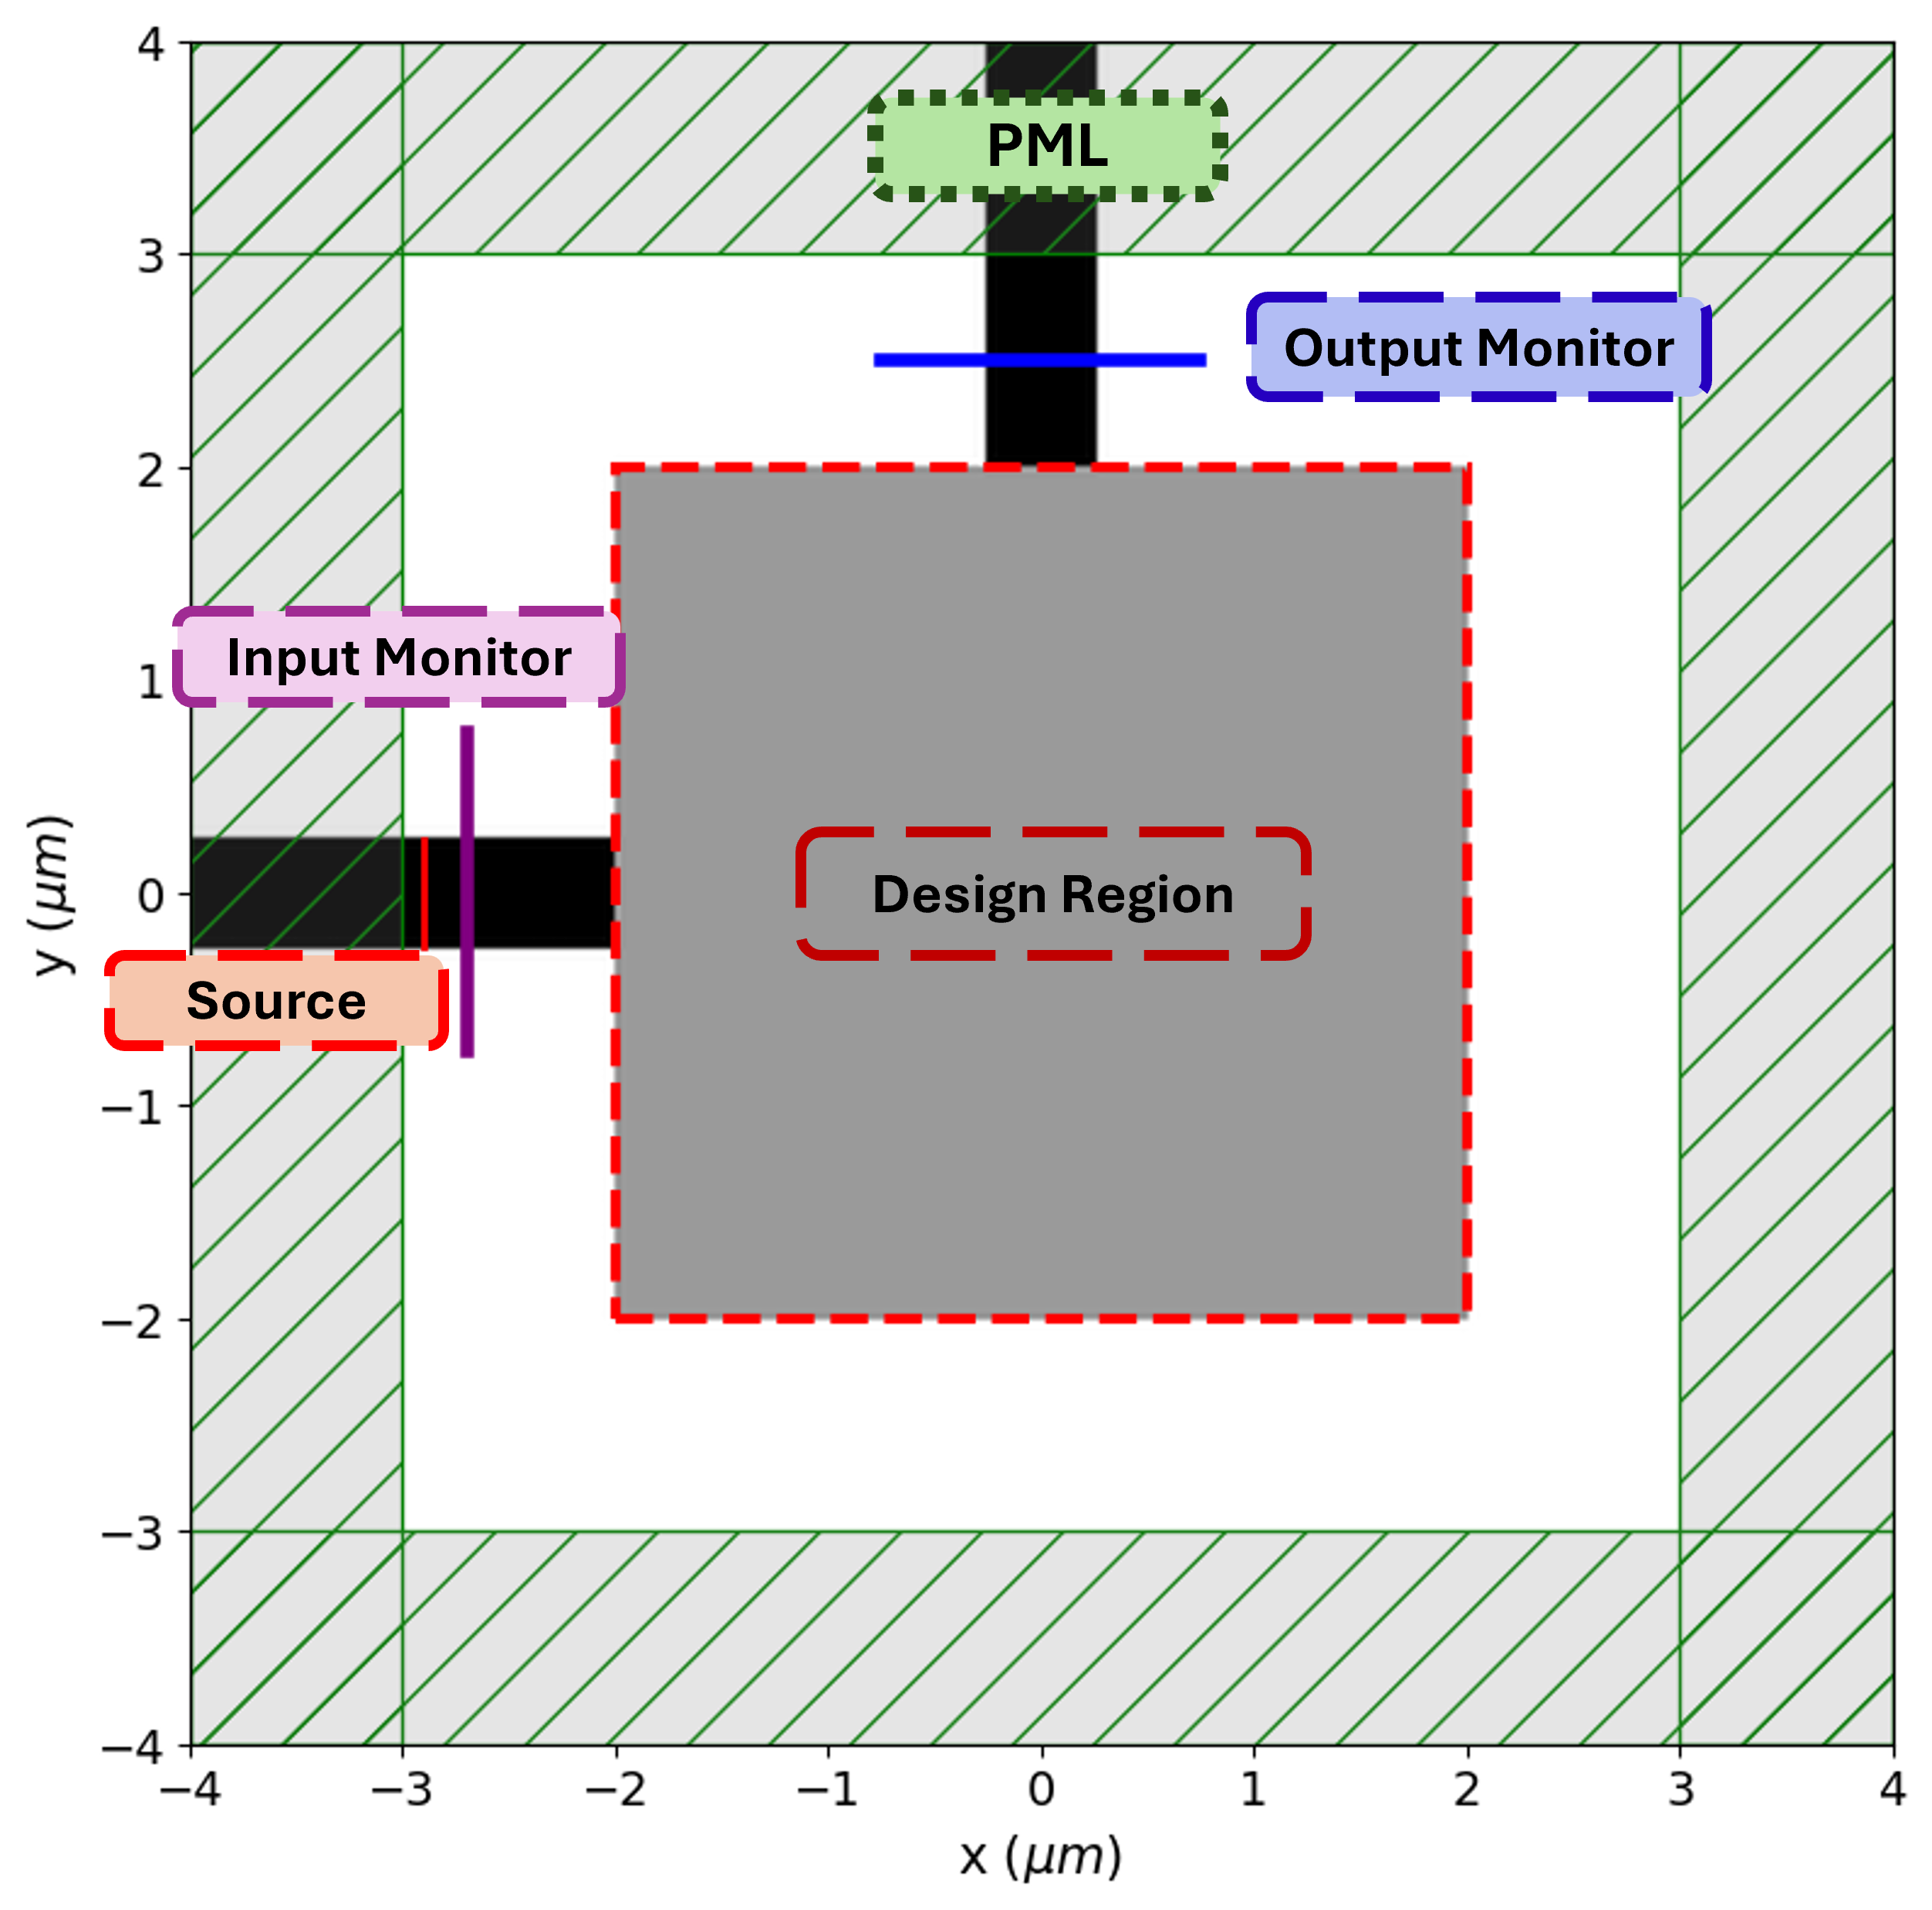
\includegraphics[width=0.8\textwidth]{img/BEND/BendWaveguide_schematic.png}
\caption{彎曲波導的輸入、輸出通道以及其幾何結構的設計區域。}
\label{fig:BEND_schematic}
\end{figure}
如圖~\ref{fig:BEND_schematic}所示，中間灰色的部分為演算法決定材料分布的設計區域，
在此模擬中，黑色代表矽(Si)材料，折射率$n_{Si}=3.48$，白色代表背景預設材料二氧化矽(SiO$_2$)，折射率$n_{SiO_2}=1.44$。
上方為光場輸出通道，以及用深藍色標示為輸出通道的模態偵測器;
左側分別為光場輸入通道、利用紫色標示為輸入通道的模態偵測器，以及用紅色標示為光場激發的起點;
在示意圖的最外圍，以深綠色標示出吸收邊界(PML)，用來吸收模擬光場，避免產生反射效應。

光源設定方面，我同樣是使用了MEEP中的EigenModeSource，利用GaussianSource高斯脈衝激發波長為$1550 nm$的光源
，以及分別設定了$\text{eig\_band}=1$ 以及 $\text{eig\_parity}=\text{mp.EVEN\_Y}$來設定要輸入到通道中的 TE$_0$模態。

本研究的設計目標為設計一個結構，並且此結構能夠將輸入通道中的 TE$_0$ 模態能量盡可能地完全傳導至輸出通道。
因此，在此研究中可以定義 Figure of Merit(FoM)作為 彎曲波導 結構的最佳化目標:
\begin{align}
FoM = T = \frac{E_{\mathrm{output}}}{E_{\mathrm{input}}}
\label{eq:BEND_FoM}
\end{align}
其中 $E_{\mathrm{output}}$ 為輸出波導中的總能量，$E_{\mathrm{input}}$ 為輸入波導中的總能量; $T$為彎曲波導的穿透率。
這邊我們的設計目標就是最大化彎曲波導的穿透率，當波導的穿透率越大，自然也會降低反射損耗與散射損耗，因此當此公式設計結果越好，其數值會越接近$1$。

\subsection{Gaussian Upsampling Strategy on Bend Waveguide Design}

\subsubsection{Gaussian Upsampling on Bend Waveguide Design - parameter 1}
\label{ch:GU_BEND_Design1}
首先，在設計彎曲波導一開始的實驗中，我們嘗試使用較少的初始訓練資料量，共200筆，以及設定30次的迭代次數，並在每次迭代後增加60筆的訓練資料，總資料量為2000筆。

接著，在設計區域為$4.0 \times 4.0 \mu m^2$中劃分網格為$8 \times 8$，因此每一個網格的尺寸為$0.5 \times 0.5 \mu m^2$。
假設最小線寬為$150nm$，我們可以透過公式\eqref{eq:sigma_pix_min}推導出高斯濾波器的標準差為0.222，為了避免過小的標準差降低幾何特徵的約束能力，
因此標準差取1。結構的部分，由於輸出輸入波導只需要允許TE$_0$模態，因此波導寬度設定為$0.5 \mu m$。

最終品質因數FOM為:
\begin{align}
FOM = 0.8277
\label{eq:BEND_FoM_Design1}
\end{align}
使用較少的資料量進行優化，初步獲得 82.77\% 的穿透率。
透過圖~\ref{fig:BEND_design1_Bestfom_vs_iteration}和圖~\ref{fig:BEND_design1_Opt_Trajactory}可以發現，
使用 $8 \times 8$ 網格劃分再透過Gaussian Upsampling進行平滑化處理的彎曲波導設計，
對於FM模型訓練以及QUBO問題的求解皆能夠有效的進行優化。
\begin{figure}[H]
\centering
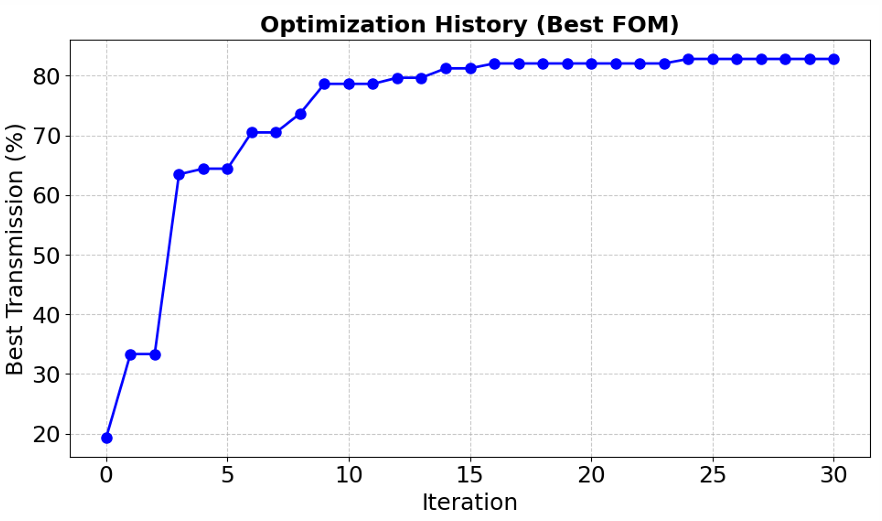
\includegraphics[width=0.8\textwidth]{img/BEND/BEND-GU-design1/BESTFOM_vs_iter.png}
\caption{Gaussian Upsampling策略於彎曲波導 Design 1最佳化過程中的最佳FoM變化。}
\label{fig:BEND_design1_Bestfom_vs_iteration}
\end{figure}

\begin{figure}[H]
\centering
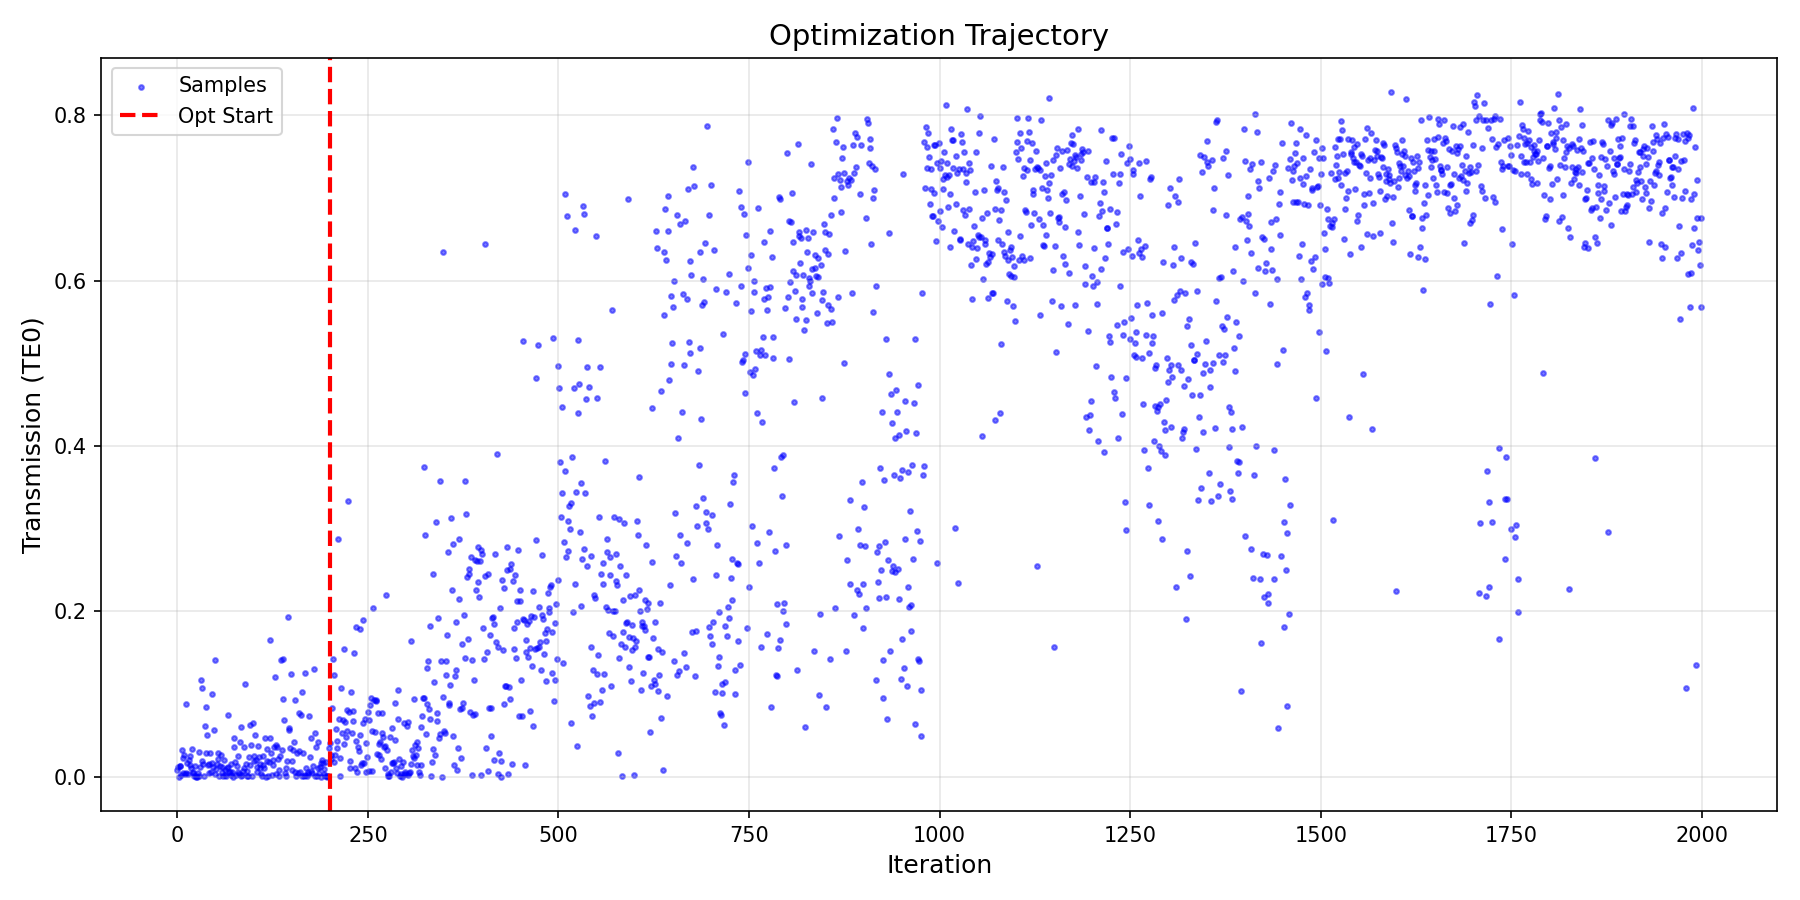
\includegraphics[width=1.0\textwidth]{img/BEND/BEND-GU-design1/transmission_trajectory.png}
\caption{Gaussian Upsampling策略於彎曲波導 Design 1最佳化過程中的FoM變化。}
\label{fig:BEND_design1_Opt_Trajactory}
\end{figure}

圖~\ref{fig:BEND_structure_design1}為最終設計出的結構圖，最終的模擬結果如圖~\ref{fig:BEND_DFT_design1}所示，
可以發現經過演算法尋找出的結構能夠有效的將光場局限於結構中(白色輪廓內)，而如何將穿透率進一步提升將是後續參數調整的方向。
\begin{figure}[H]
\centering
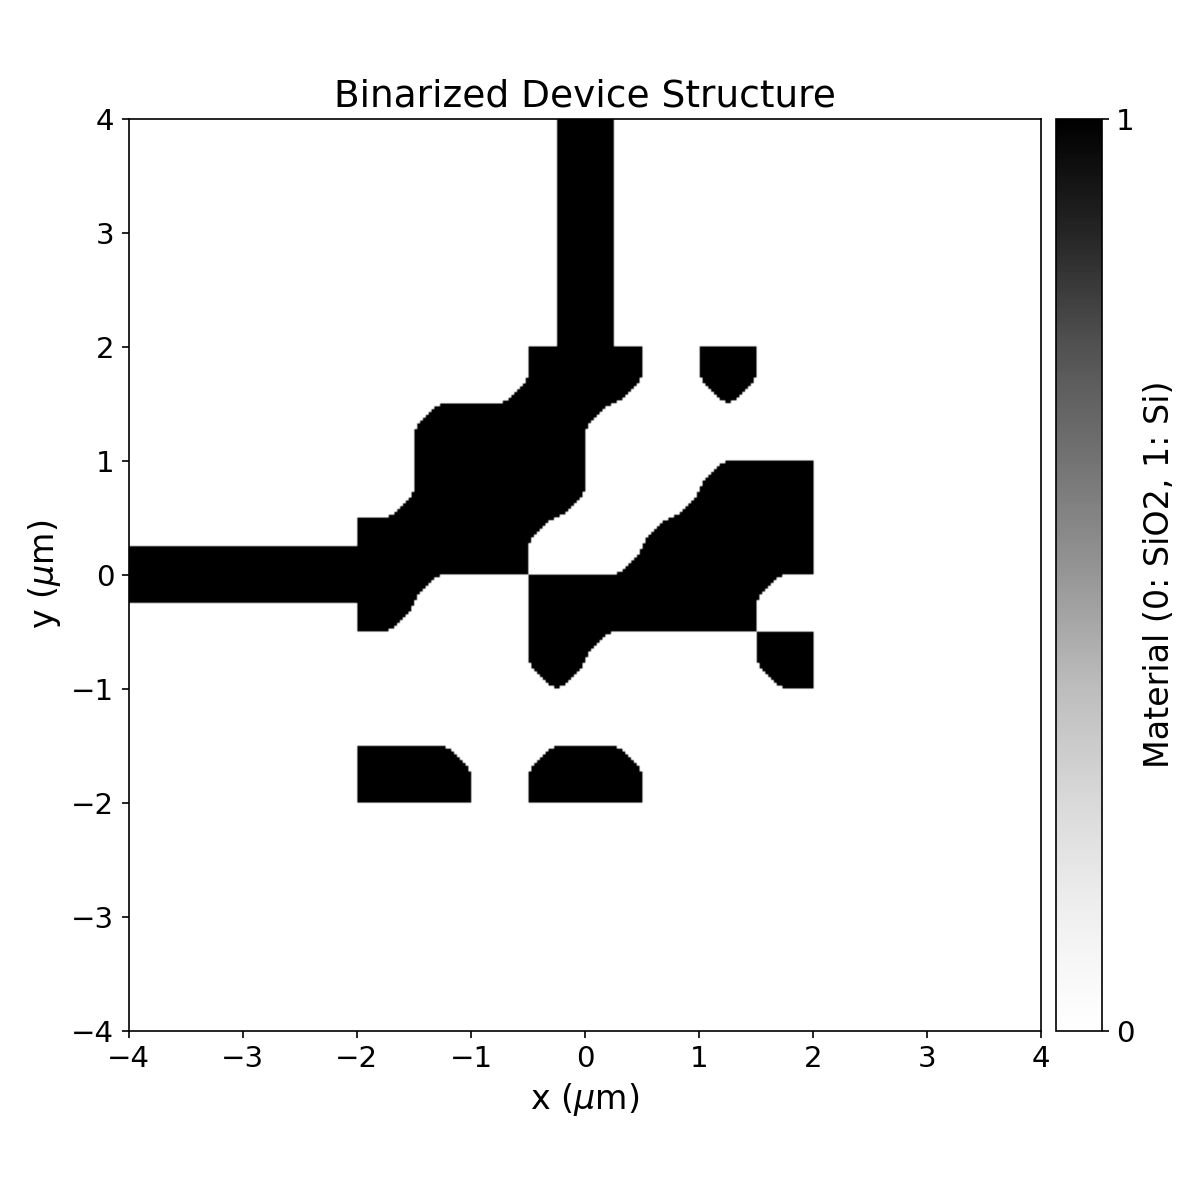
\includegraphics[width=0.7\textwidth]{img/BEND/BEND-GU-design1/eval_TE0_structure_binary.png}
\caption{彎曲波導 Design 1之幾何結構圖。}
\label{fig:BEND_structure_design1}
\end{figure}

\begin{figure}[H]
\centering
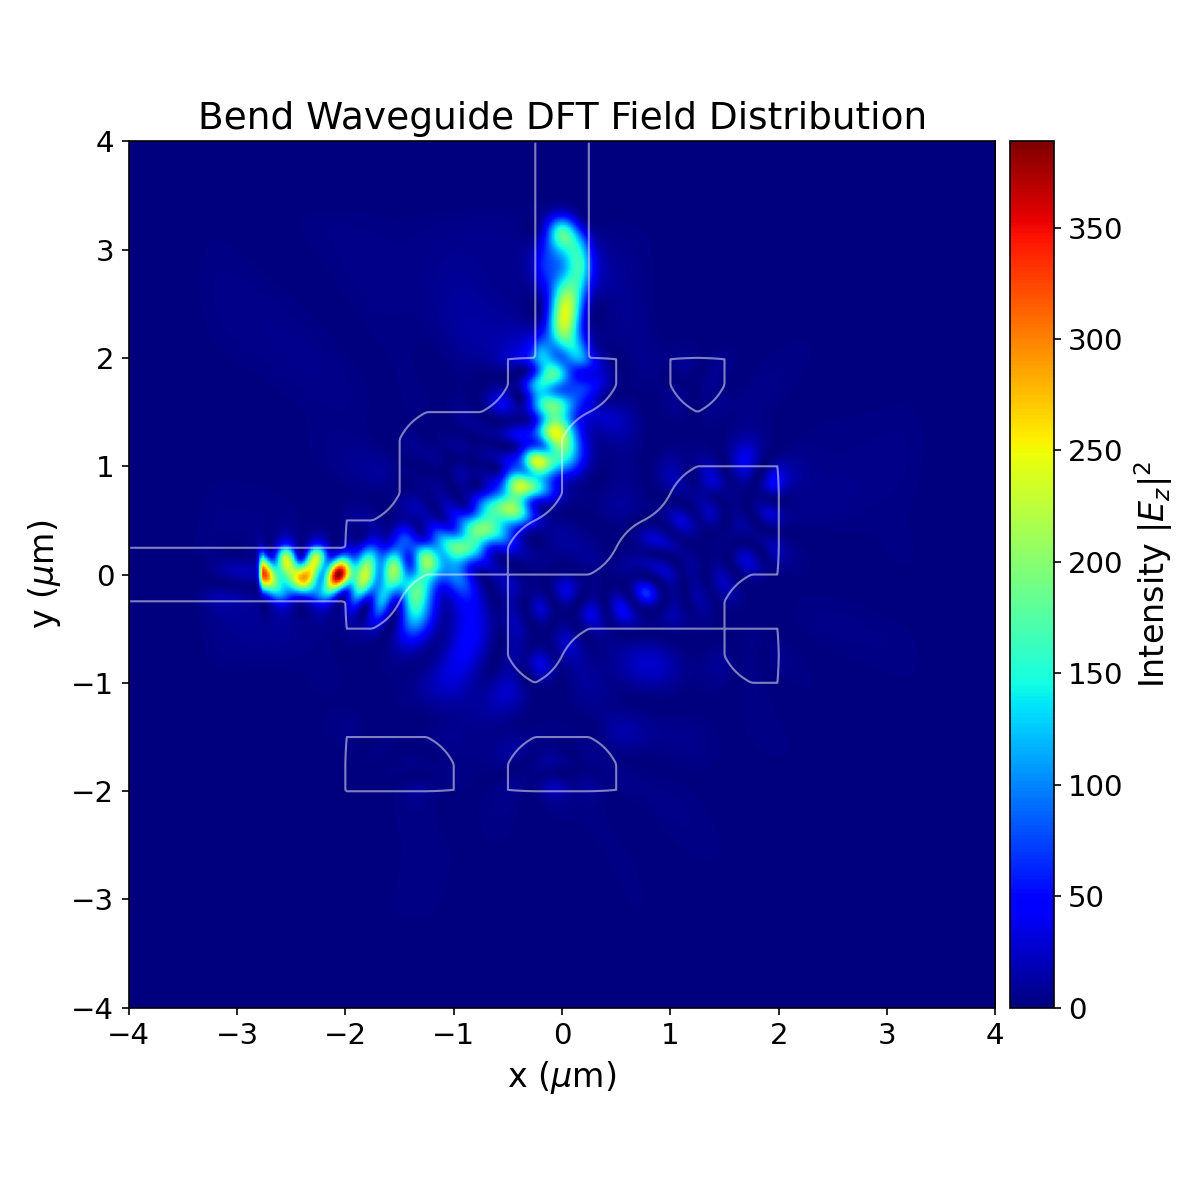
\includegraphics[width=0.8\textwidth]{img/BEND/BEND-GU-design1/eval_TE0_field.png}
\caption{彎曲波導 Design 1之DFT電場強度分布圖。}
\label{fig:BEND_DFT_design1}
\end{figure}

\subsubsection{Gaussian Upsampling on Bend Waveguide Design - parameter 2}
\label{ch:GU_BEND_Design2}
接著，我將網格劃分增加為$10 \times 10$，也就是模擬退火將在$2^{100}$個可能的結構中進行搜尋，並且將初始隨機資料量增加為1000筆，
迭代次數增加為100次，每次迭代增加30筆候選解，因此總共會有4000筆資料數。

在MEEP光源設定、結構參數設定以及Gaussian Upsampling中的標準差與高斯核設定皆與前一個實驗(第~\ref{ch:GU_BEND_Design1}節)相同。

最終品質因數FOM提升為:
\begin{align}
FOM = 0.9524
\label{eq:BEND_FoM_Design2}
\end{align}
在增加網格劃分以及總資料量後，彎曲波導的穿透率提升至95.24\%。
透過圖~\ref{fig:BEND_design2_Bestfom_vs_iteration}中可以發現，雖然演算法在第40次迭代就停止了搜尋，
但在圖~\ref{fig:BEND_design2_Opt_Trajactory}中可以觀察到最佳化過程中的整體趨勢仍然持續上升。
\begin{figure}[H]
\centering
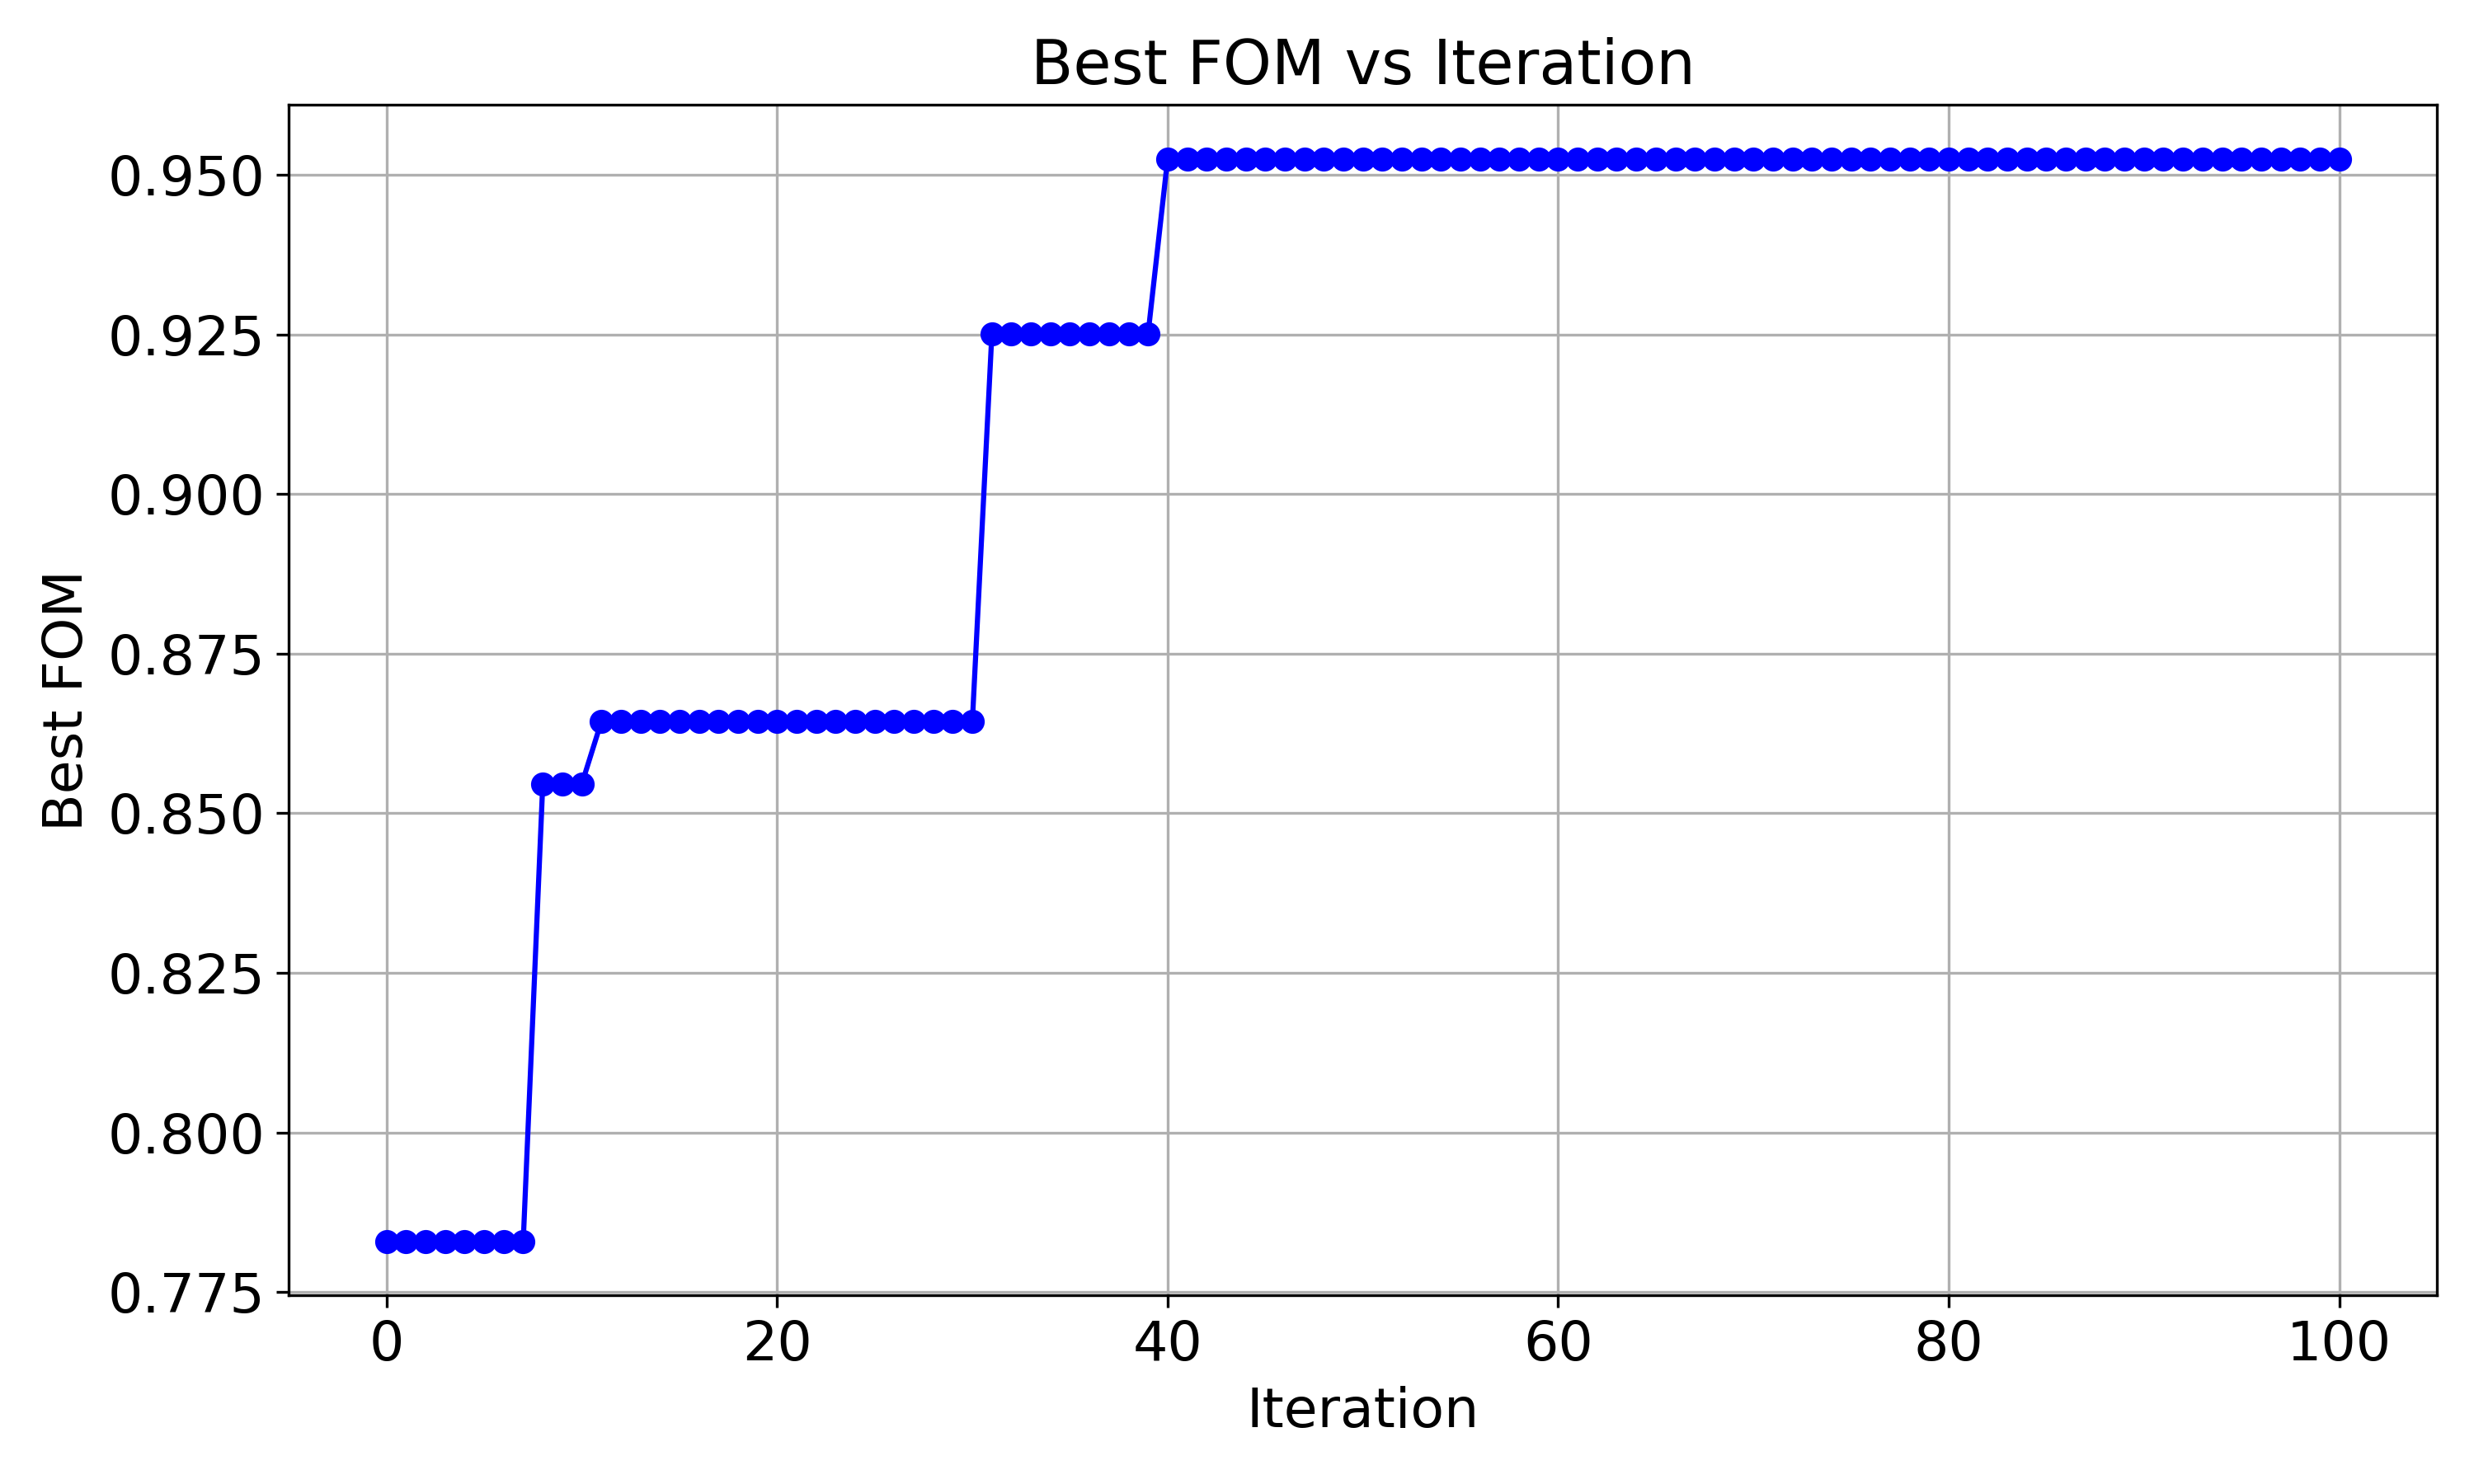
\includegraphics[width=0.8\textwidth]{img/BEND/BEND-GU-design2/fom_evolution.png}
\caption{彎曲波導 Design 2最佳化過程中的最佳FoM變化。}
\label{fig:BEND_design2_Bestfom_vs_iteration}
\end{figure}

\begin{figure}[H]
\centering
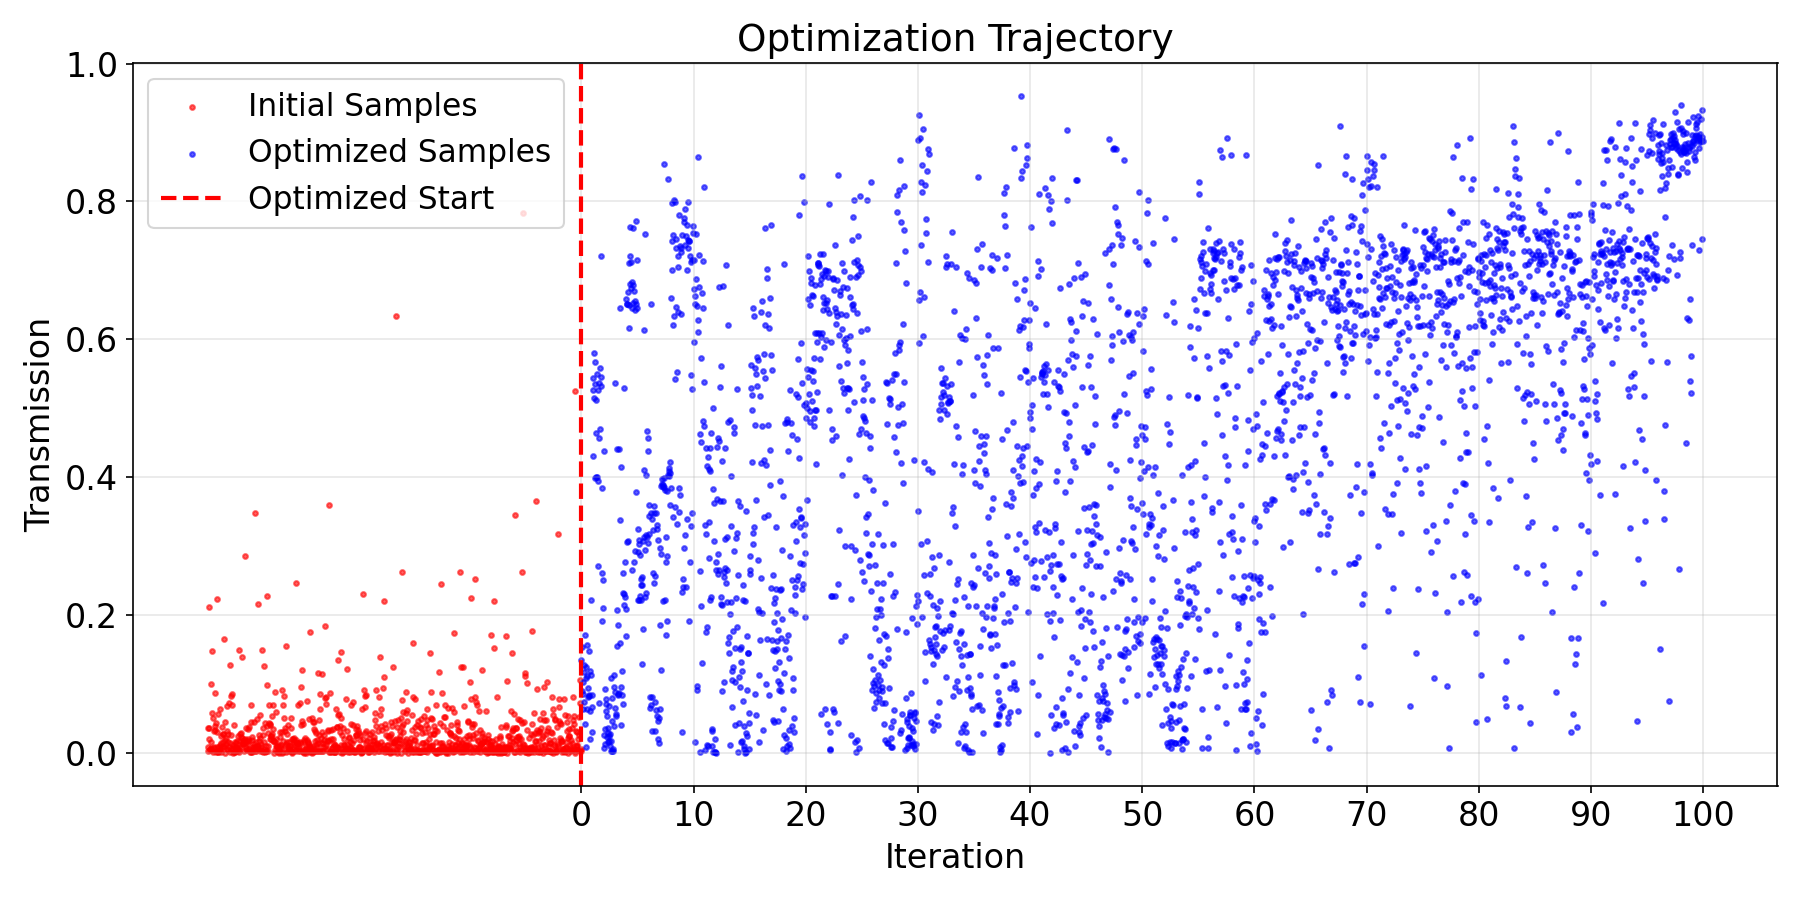
\includegraphics[width=0.8\textwidth]{img/BEND/BEND-GU-design2/transmission_trajectory.png}
\caption{彎曲波導 Design 2最佳化過程中的FoM變化。}
\label{fig:BEND_design2_Opt_Trajactory}
\end{figure}

圖~\ref{fig:BEND_DFT_design2}呈現出了優化後90度彎曲波導的電場強度($\vert{}E_z\vert{}^2$)分布。
觀察光場分布可發現，光波在通過彎曲段的不規則結構時，模態雖然會產生暫時性的畸變，但在進入直線輸出波導後，
光場能夠重新收斂並完成模態耦合，最終於輸出端仍然能夠維持完整且對稱的模態分布。
\begin{figure}[H]
\centering
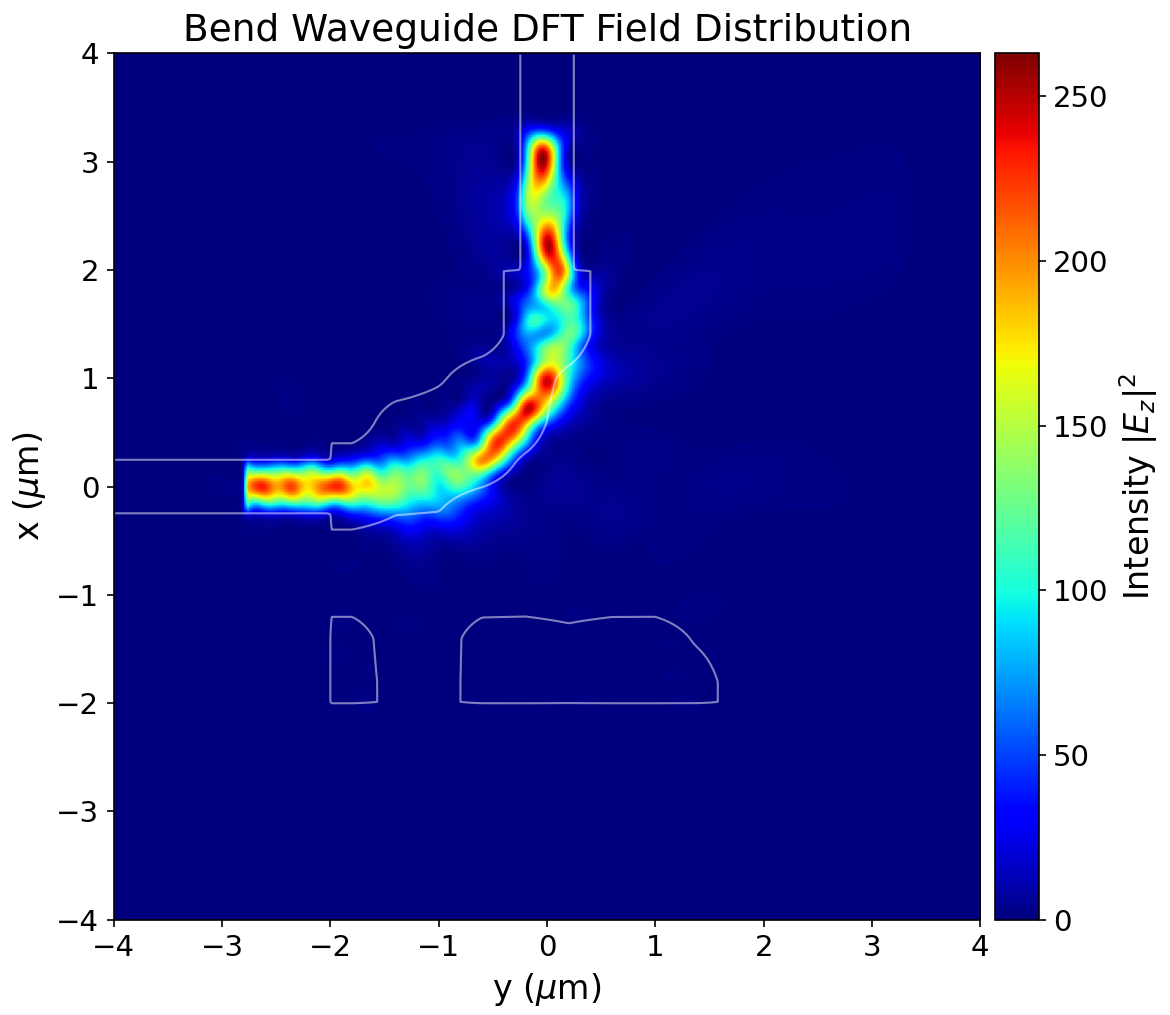
\includegraphics[width=0.8\textwidth]{img/BEND/BEND-GU-design2/eval_TE0_field.png}
\caption{彎曲波導 Design 2之DFT電場強度分布圖。}
\label{fig:BEND_DFT_design2}
\end{figure}
從圖~\ref{fig:BEND_structure_design2}中可以發現，此現象可以歸咎於演算法在輸入與輸出波導交界處所演化出的絕熱結構(Adiabatic Structures)。
透過適當的幾何漸變設計，絕熱過渡區域可以提供平滑的模態轉換，降低因為幾何突變所產生的反射與散射損耗，
使光場能夠有效傳輸至輸出端，進而維持高穿透率及良好的模態品質。
\begin{figure}[H]
\centering
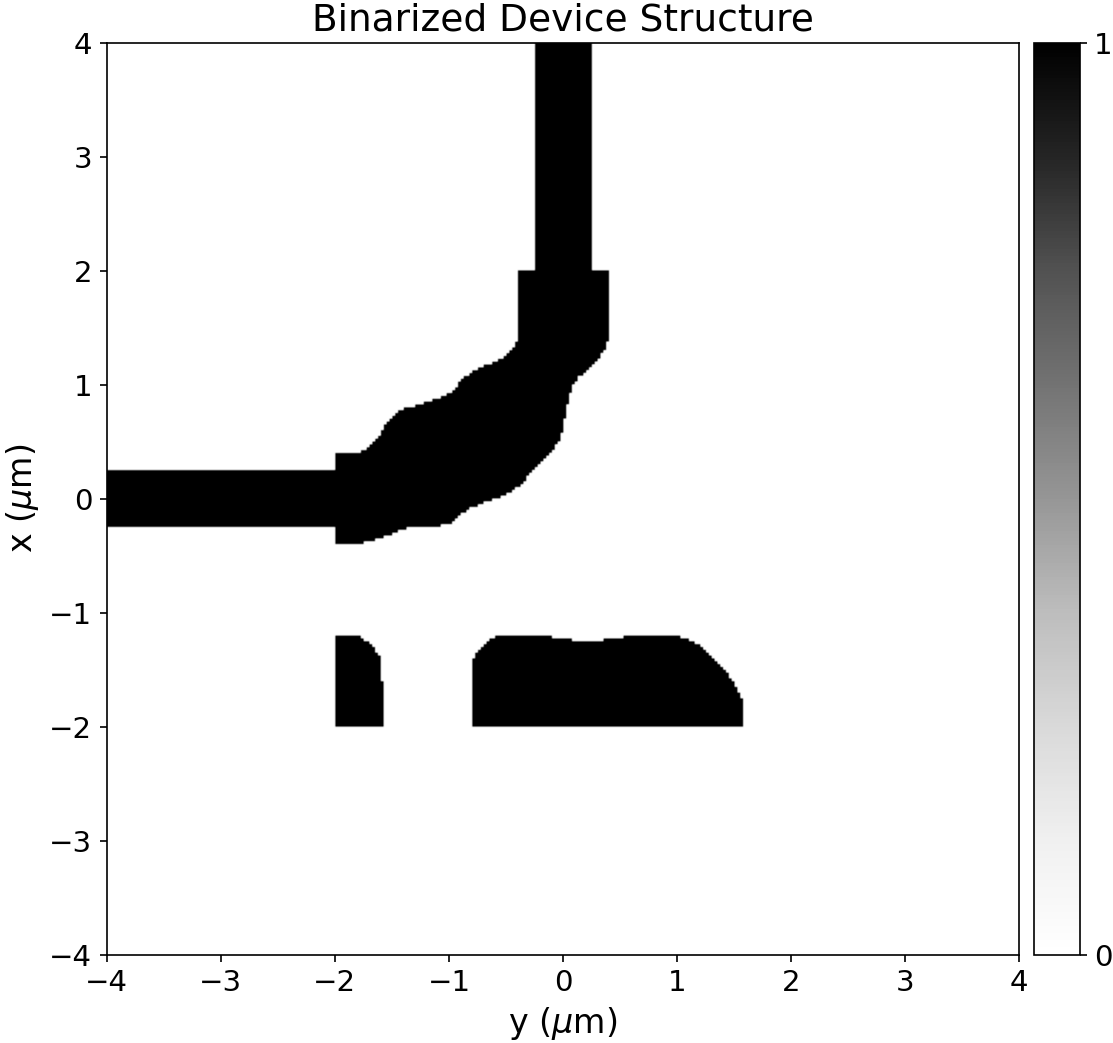
\includegraphics[width=0.7\textwidth]{img/BEND/BEND-GU-design2/eval_TE0_structure_binary.png}
\caption{彎曲波導 Design 2之幾何結構圖。}
\label{fig:BEND_structure_design2}
\end{figure}

\subsubsection{Gaussian Upsampling on Bend Waveguide Design - parameter 3}
\label{ch:GU_BEND_Design3}
接著，我將網格劃分設定進一步增加為$12 \times 12$，提供演算法更高的結構設計自由度。
為了公平比較不同設計網格的最佳化效果，此實驗維持與前一個實驗(第~\ref{ch:GU_BEND_Design2}節)相同的資料設定，
初始隨機資料量為 1000 筆，並進行 100 次迭代，每次迭代新增 30 筆候選解，因此最終總資料量為 4000 筆。

此外，MEEP 模擬中的光源設定、結構參數，以及 Gaussian Upsampling 所使用的高斯標準差與高斯核大小，
皆與彎曲波導第一個實驗(第~\ref{ch:GU_BEND_Design1}節)保持一致，以確保不同設計網格間的比較僅反映設計變數維度增加所帶來的影響。

品質因數FOM提升為:
\begin{align}
FOM = 0.9555
\label{eq:BEND_FoM_Design3}
\end{align}
最終的穿透率提升至$95.55\%$，與前一個實驗(第~\ref{ch:GU_BEND_Design2}節)相比，
增加了$0.31\%$。整體而言，這也是Gaussian Upsampling方法應用於彎曲波導設計的效能顛峰。

雖然由圖~\ref{fig:BEND_design3_Bestfom_vs_iteration}可觀察到，FoM 隨著迭代次數增加而穩定提升，
但由圖~\ref{fig:BEND_design3_Opt_Trajactory}可發現與圖~\ref{fig:BEND_design2_Opt_Trajactory}有所不同。
相較於Design2的圖~\ref{fig:BEND_design2_Opt_Trajactory}在最佳化後期出現大量候選解集中於相近 FoM 區間的現象，
圖~\ref{fig:BEND_design3_Opt_Trajactory}的候選解則呈現較為分散的分布，顯示演算法在後期仍持續探索不同的解空間，而尚未完全收斂至特定區域。
此現象可能與設計變數增加至 $12 \times 12$ 後，使搜尋空間更加龐大且複雜有關，因此在相同資料量下，代理模型較難快速聚焦於較佳解。
\begin{figure}[H]
\centering
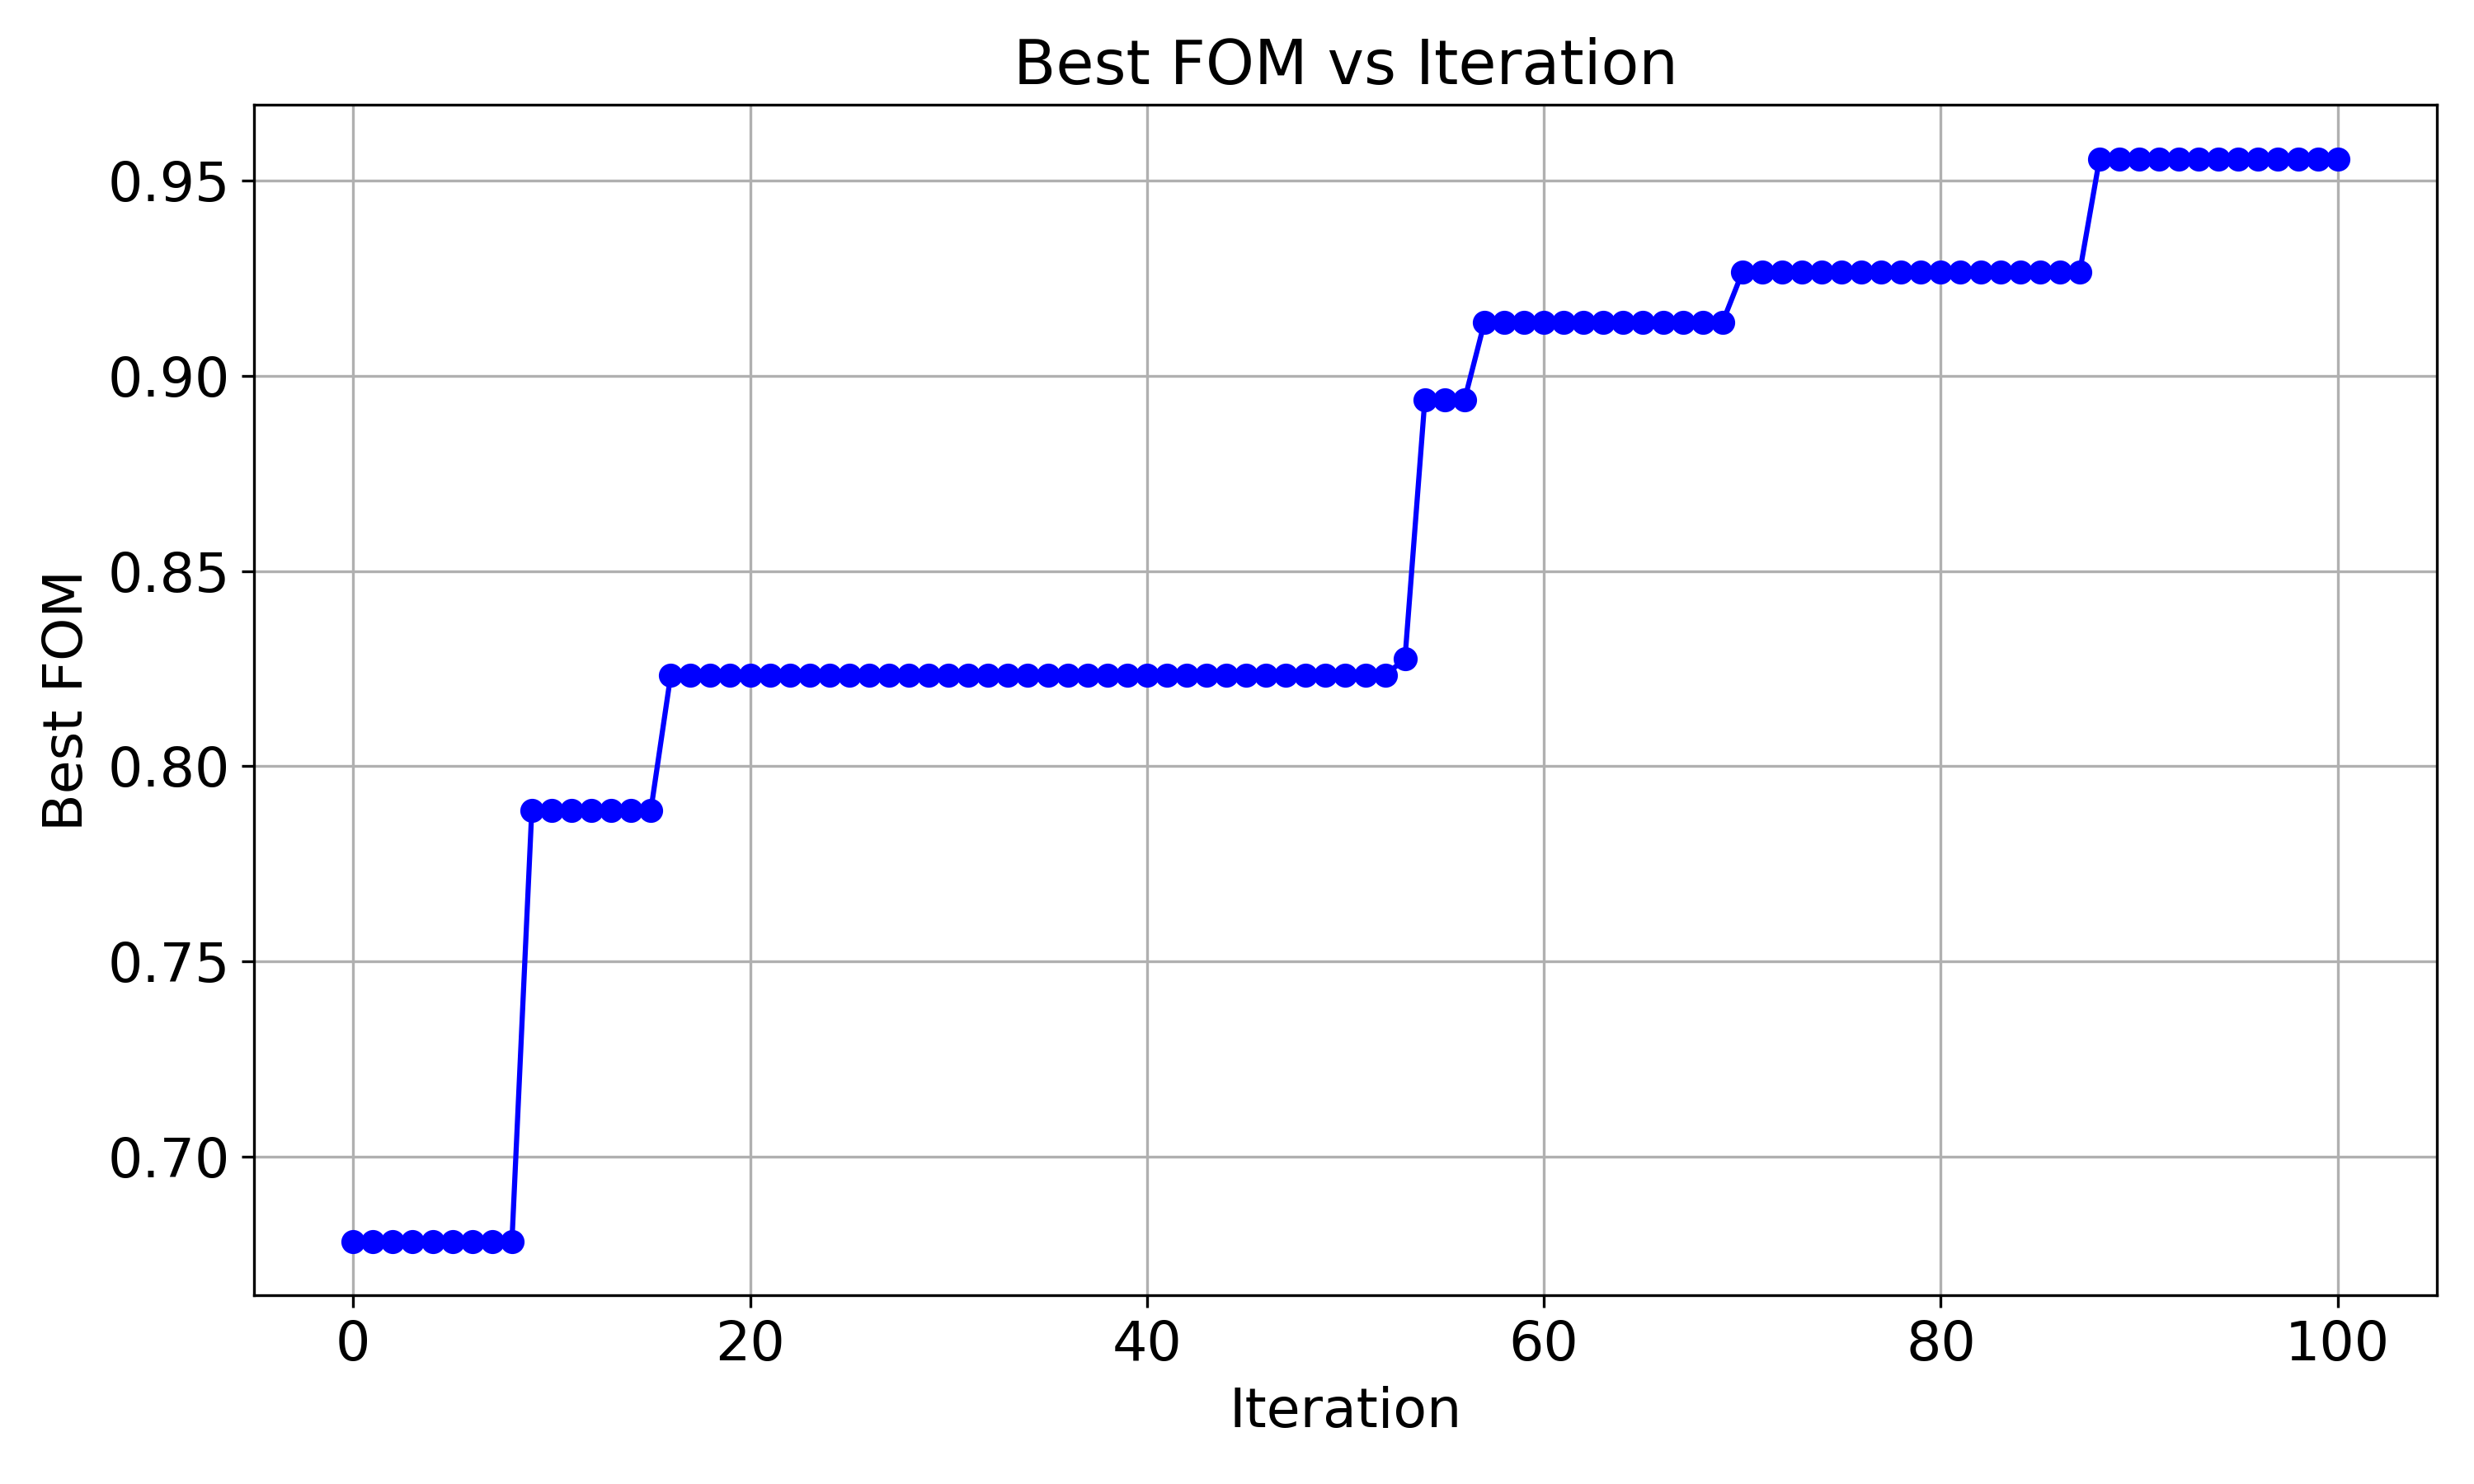
\includegraphics[width=0.8\textwidth]{img/BEND/BEND-GU-design3/fom_evolution.png}
\caption{彎曲波導 Design 3最佳化過程中的最佳FoM變化。}
\label{fig:BEND_design3_Bestfom_vs_iteration}
\end{figure}
\begin{figure}[H]
\centering
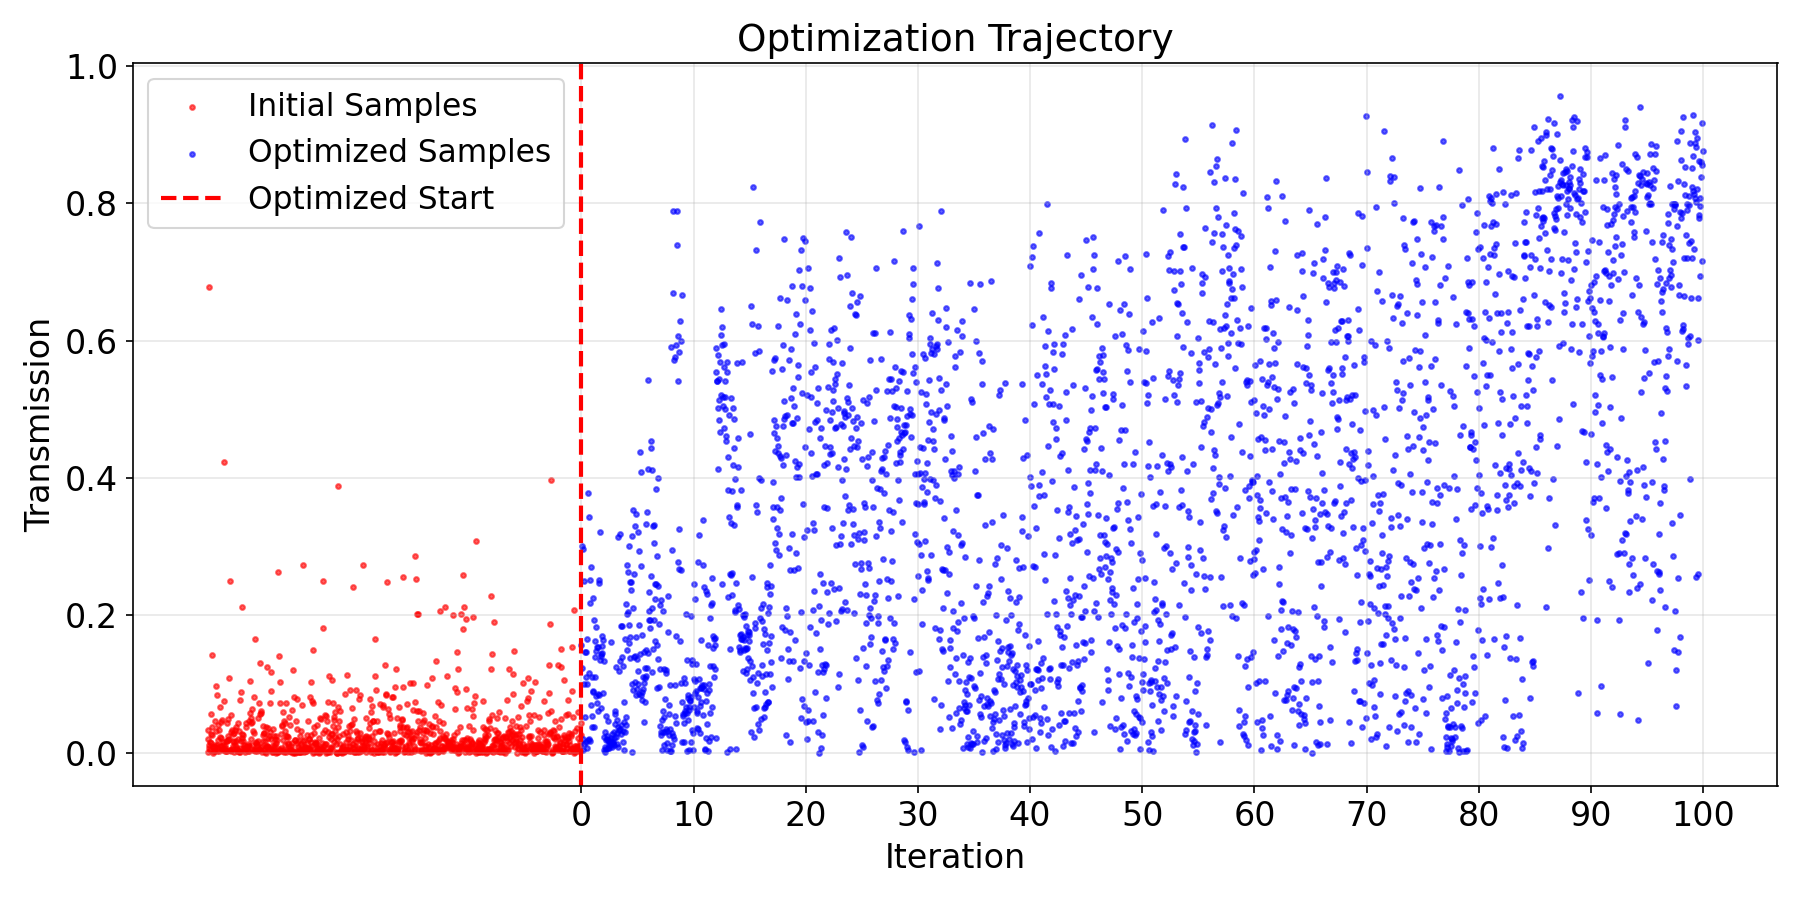
\includegraphics[width=0.8\textwidth]{img/BEND/BEND-GU-design3/transmission_trajectory.png}
\caption{彎曲波導 Design 3最佳化過程中的FoM變化。}
\label{fig:BEND_design3_Opt_Trajactory}
\end{figure}
圖~\ref{fig:BEND_DFT_design3}及圖~\ref{fig:BEND_structure_design3}呈現出了優化後90度彎曲波導的電場強度($\vert{}E_z\vert{}^2$)分布以及幾何結構圖。
\begin{figure}[H]
\centering
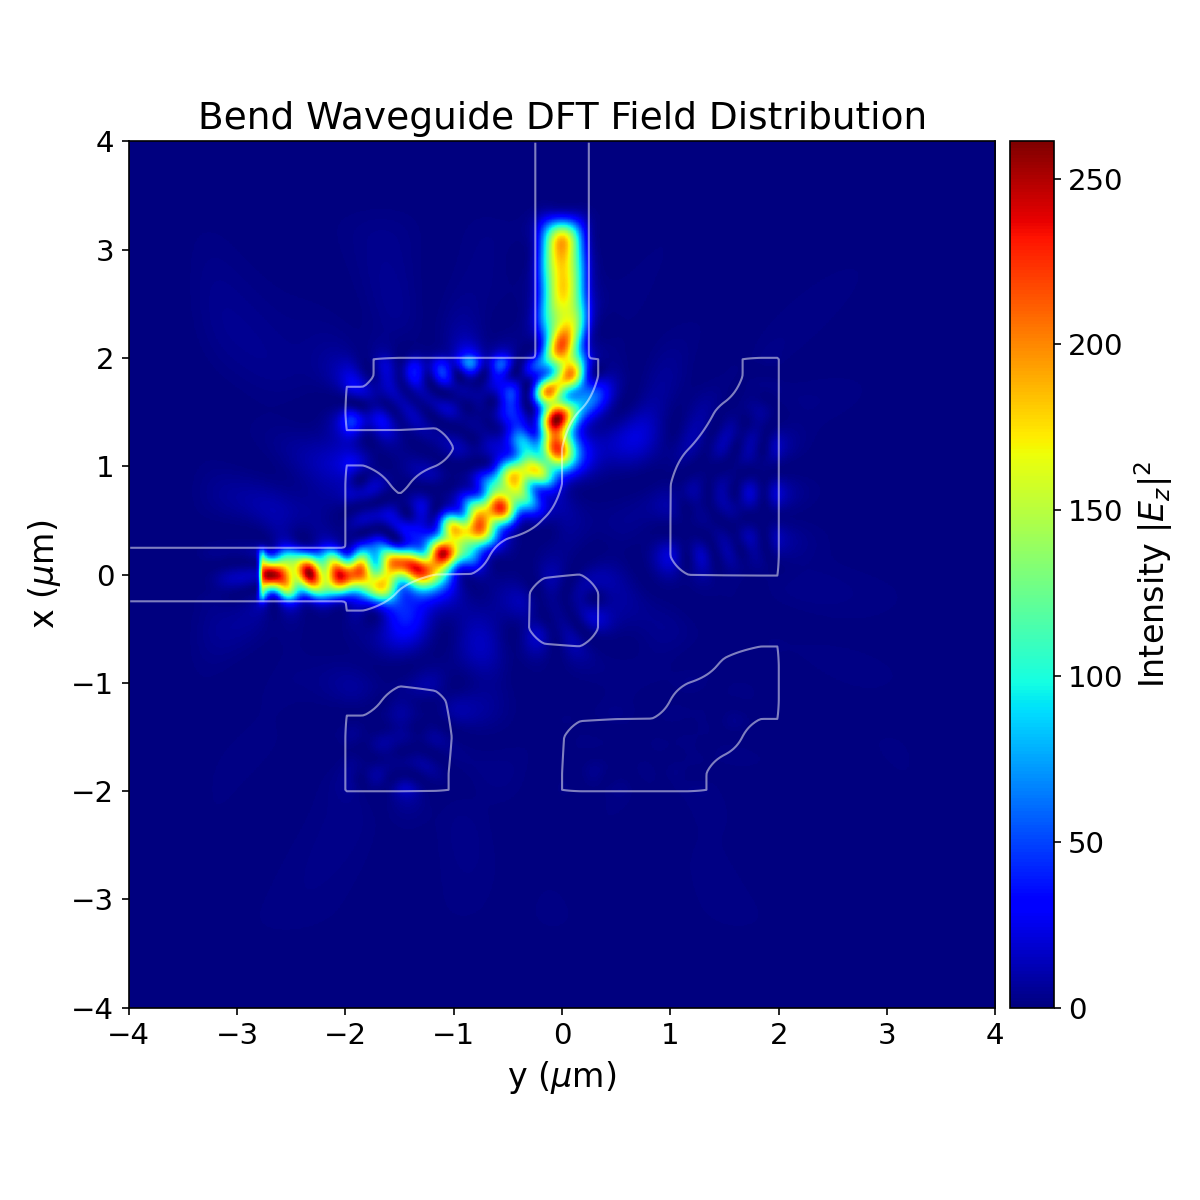
\includegraphics[width=0.8\textwidth]{img/BEND/BEND-GU-design3/eval_TE0_field.png}
\caption{彎曲波導 Design 3之DFT電場強度分布圖。}
\label{fig:BEND_DFT_design3}
\end{figure}
\begin{figure}[H]
\centering
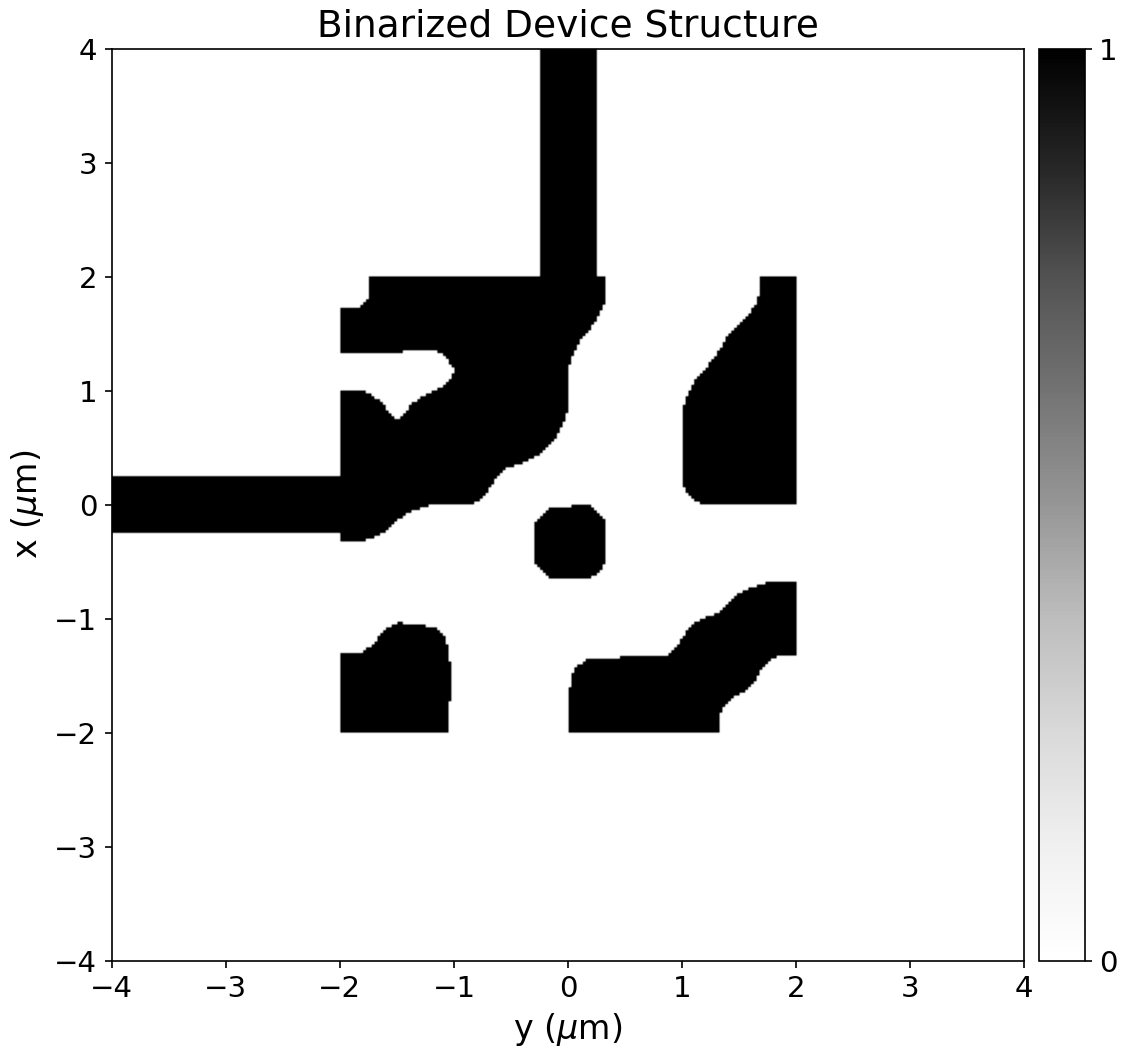
\includegraphics[width=0.7\textwidth]{img/BEND/BEND-GU-design3/eval_TE0_structure_binary.png}
\caption{彎曲波導 Design 3之幾何結構圖。}
\label{fig:BEND_structure_design3}
\end{figure}

\subsubsection{Gaussian Upsampling on Bend Waveguide Design - parameter 4}
接著，將設計網格由 $12 \times 12$ 提升至 $16 \times 16$，以進一步增加設計變數的維度，探討提升設計變數維度後對彎曲波導最佳化結果的影響。
除了設計網格外，其餘 MEEP 模擬參數、Gaussian Upsampling 參數及最佳化設定皆與前一實驗相同，以確保比較結果僅反映設計自由度增加所帶來的影響。

此實驗的最佳品質因數FoM為:
\begin{align}
FOM = 0.9429
\label{eq:BEND_FoM_Design4}
\end{align}
雖然仍維持超過94\%的穿透率，但與$12 \times 12$的設計相比略為下降，顯示持續增加設計自由度並未帶來更佳的最佳化結果。

由圖~\ref{fig:BEND_design4_Opt_Trajactory}可以觀察到，初始樣本主要集中於低FoM區域，而隨著迭代進行，候選解逐漸向高FoM區域移動，
表示代理模型還是能夠有效引導搜尋方向。然而，相較於較低維度之設計，16×16設計的候選解分布仍然是較為分散，
可能是由於設計變數增加使搜尋空間擴大，因此或許在固定資料量下需要更多探索才能達到穩定收斂。
\begin{figure}[H]
\centering
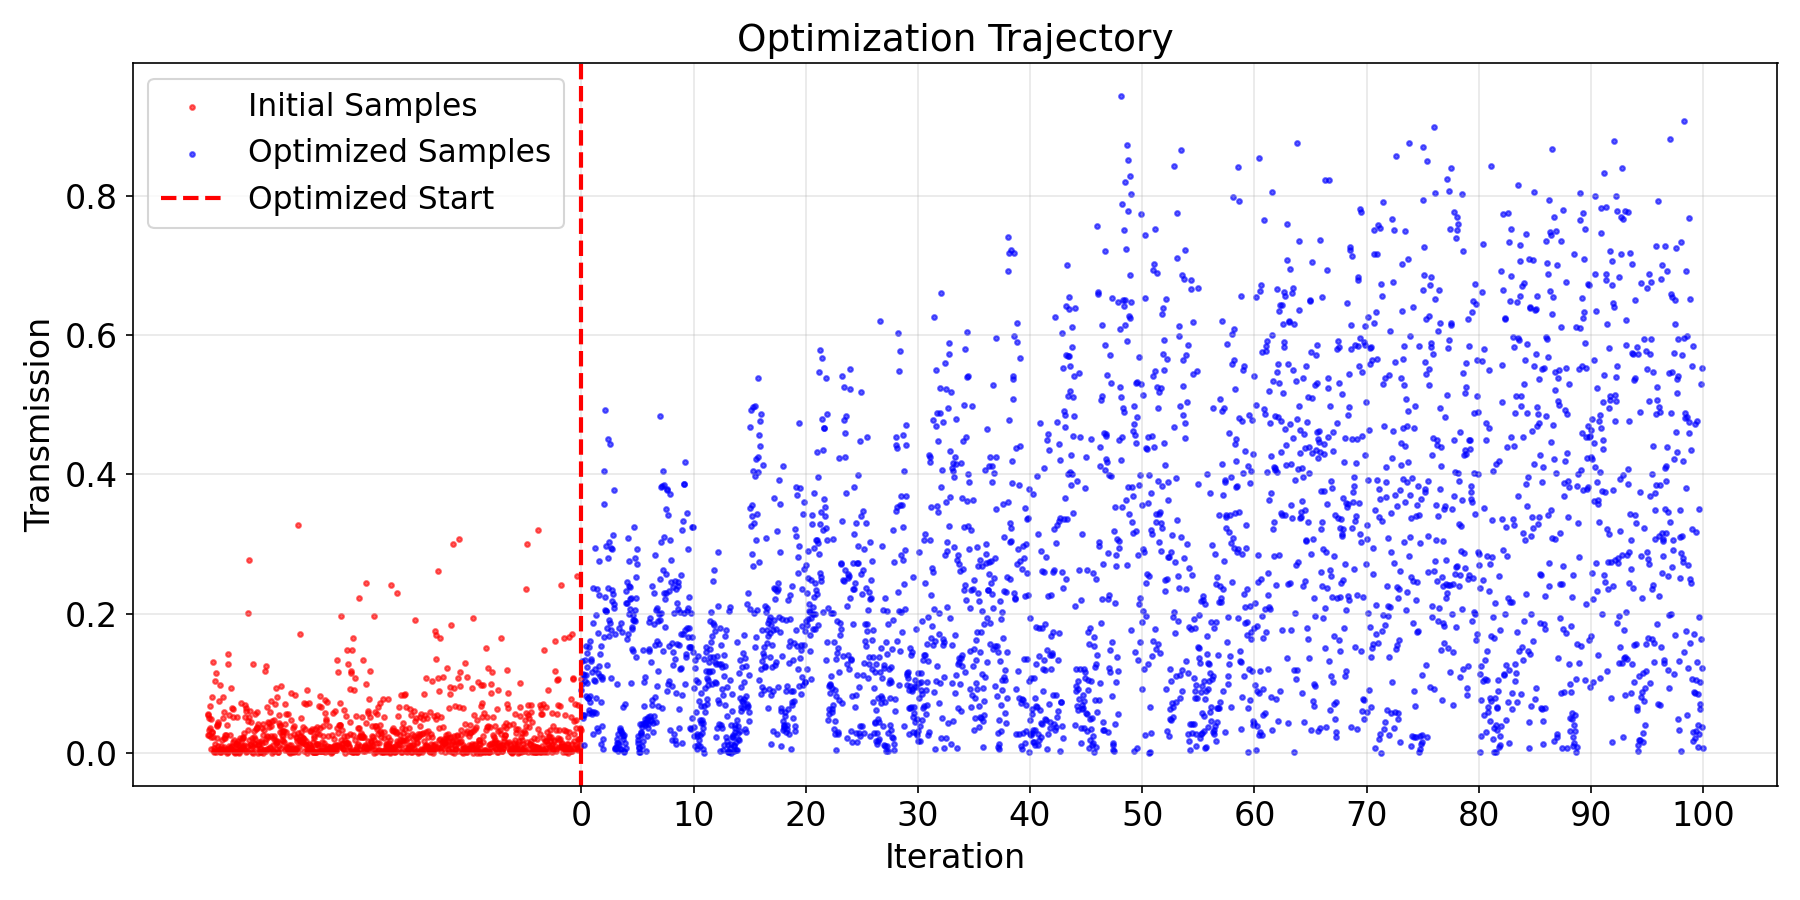
\includegraphics[width=0.8\textwidth]{img/BEND/BEND-GU-design4/transmission_trajectory.png}
\caption{彎曲波導 Design 4最佳化過程中的FoM變化。}
\label{fig:BEND_design4_Opt_Trajactory}
\end{figure}

由圖~\ref{fig:BEND_design4_Bestfom_vs_iteration}可觀察到，$16 \times 16$設計之最佳FoM隨迭代次數增加呈現階梯式提升趨勢，
代表演算法能持續更新歷史最佳候選解。初始階段由於仍處於設計空間探索階段，因此FoM提升較為緩慢，大約在第50次迭代之後，
最佳FoM快速提升並突破0.9，最終達到0.9429。
\begin{figure}[H]
\centering
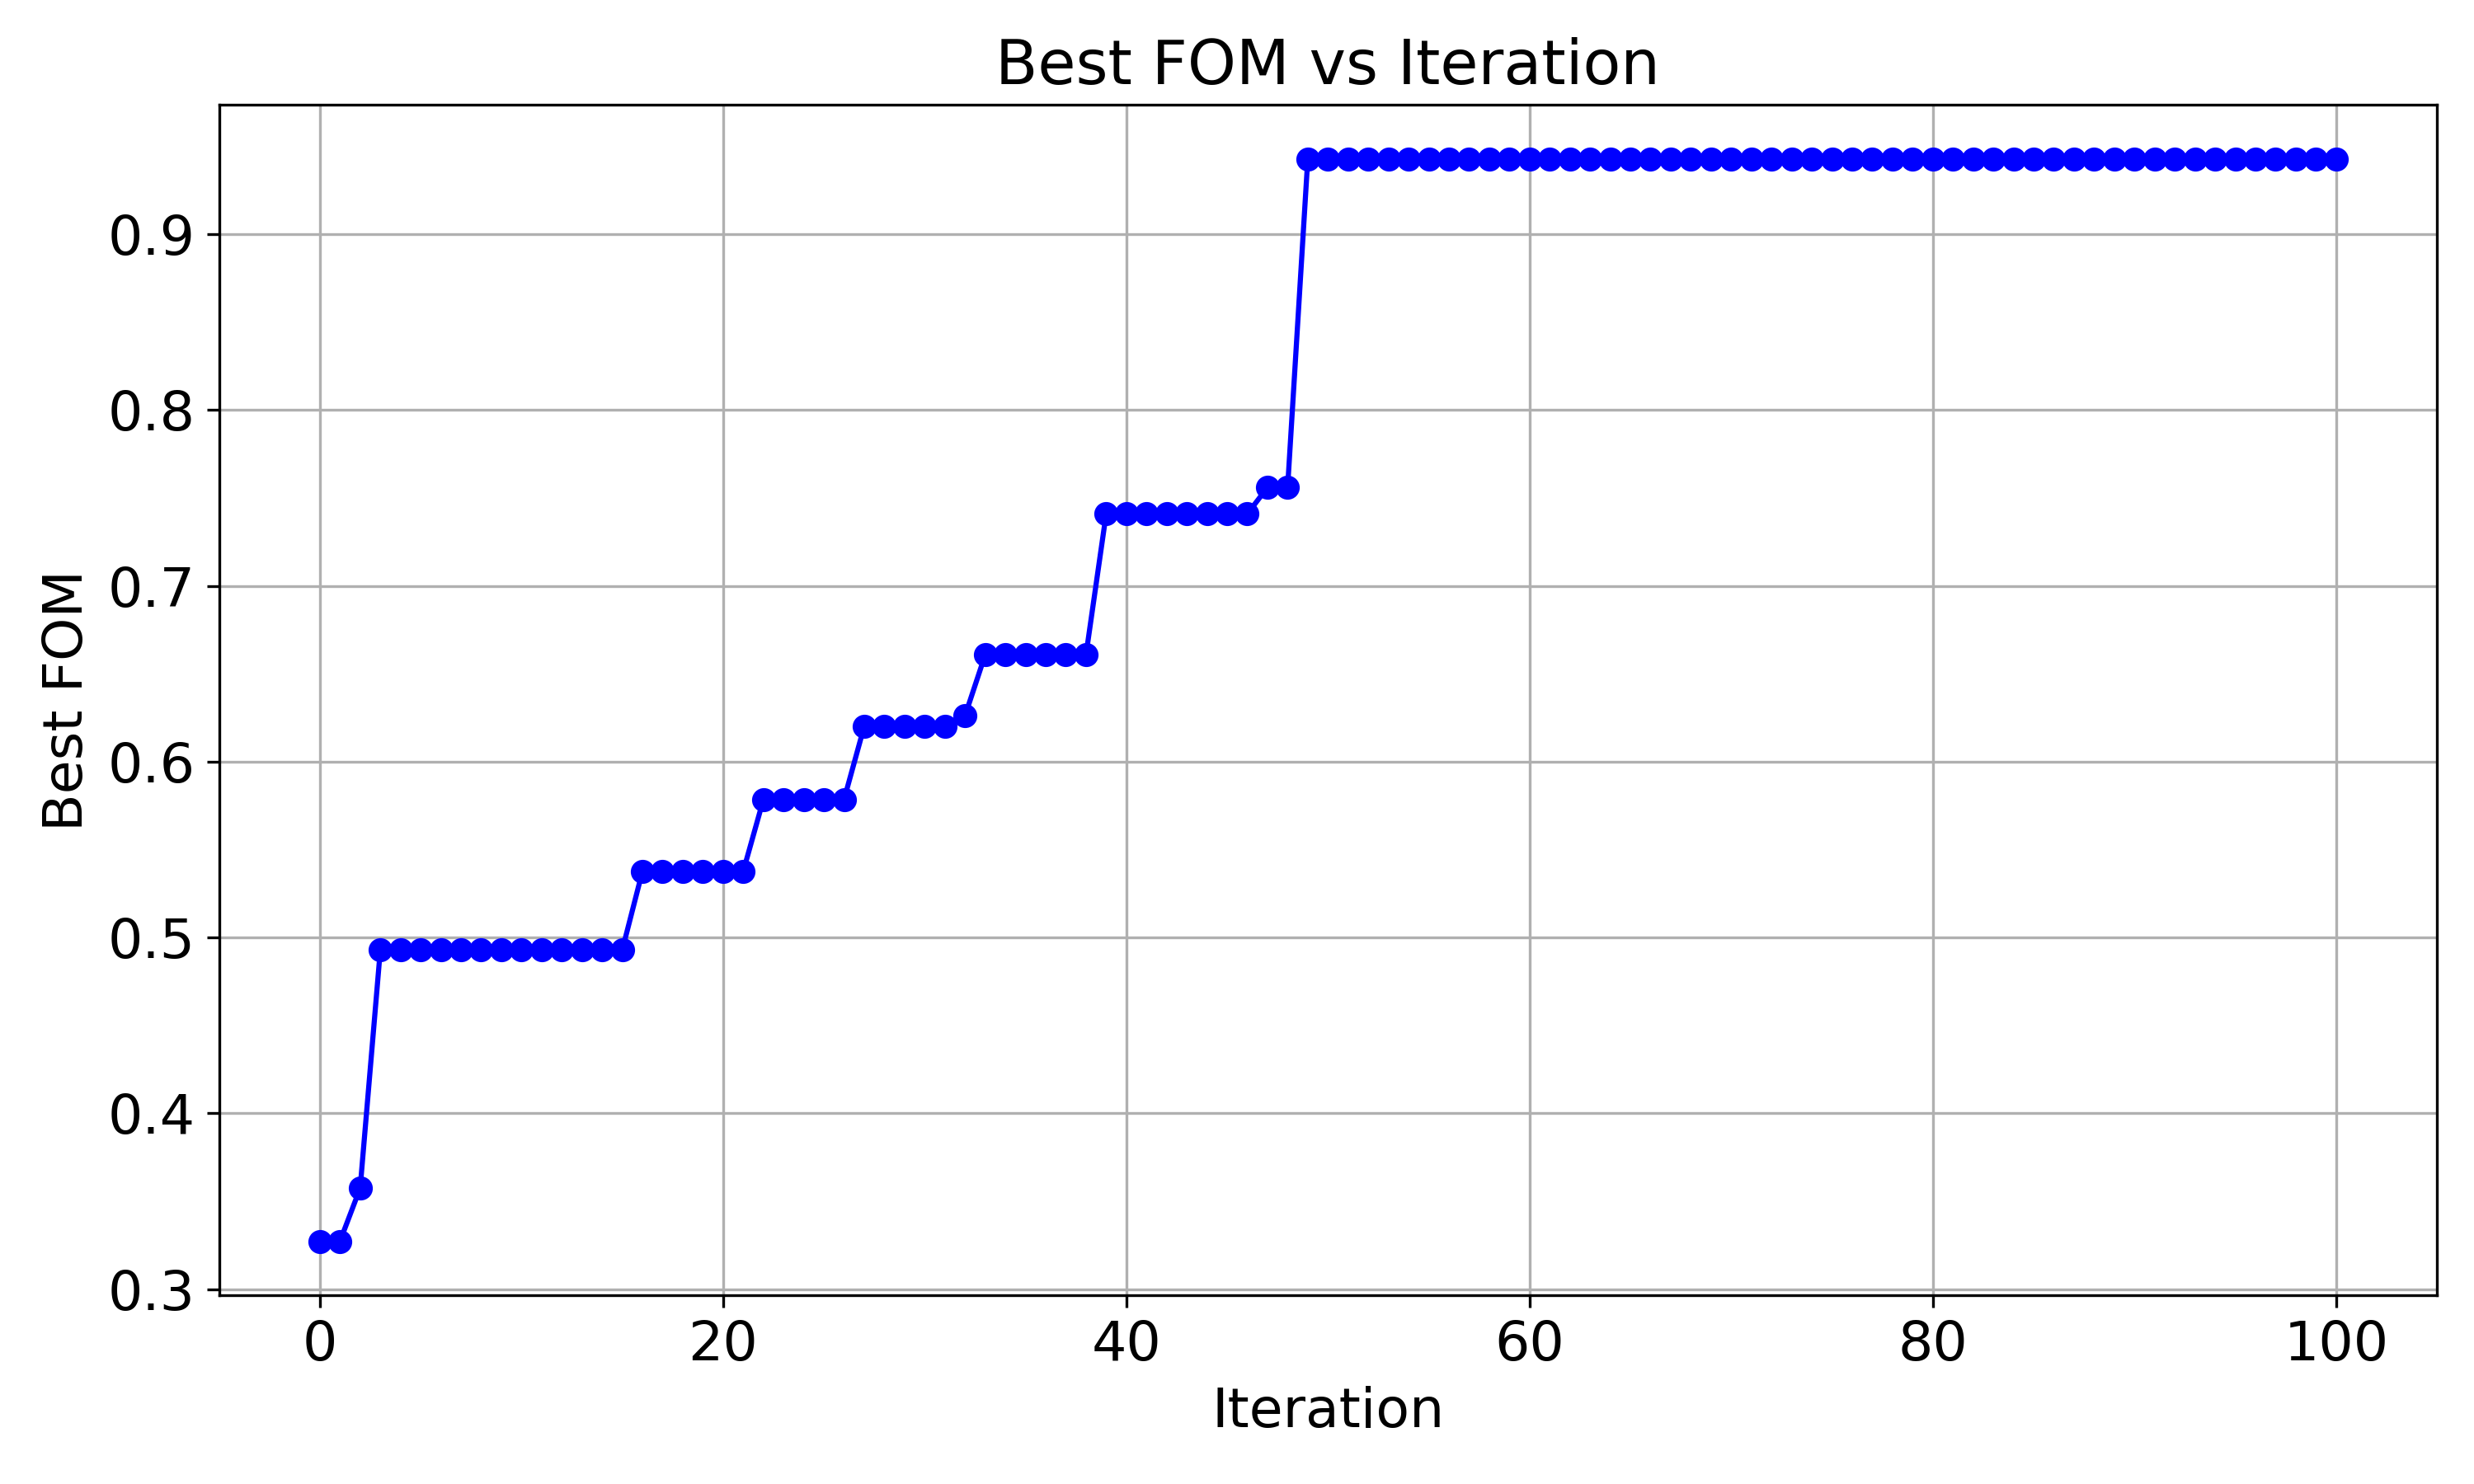
\includegraphics[width=0.8\textwidth]{img/BEND/BEND-GU-design4/fom_evolution.png}
\caption{彎曲波導 Design 4最佳化過程中的最佳FoM變化。}
\label{fig:BEND_design4_Bestfom_vs_iteration}
\end{figure}

圖~\ref{fig:BEND_DFT_design4}及圖~\ref{fig:BEND_structure_design4}呈現出了優化後90度彎曲波導的電場強度($\vert{}E_z\vert{}^2$)分布以及幾何結構圖。
\begin{figure}[H]
\centering
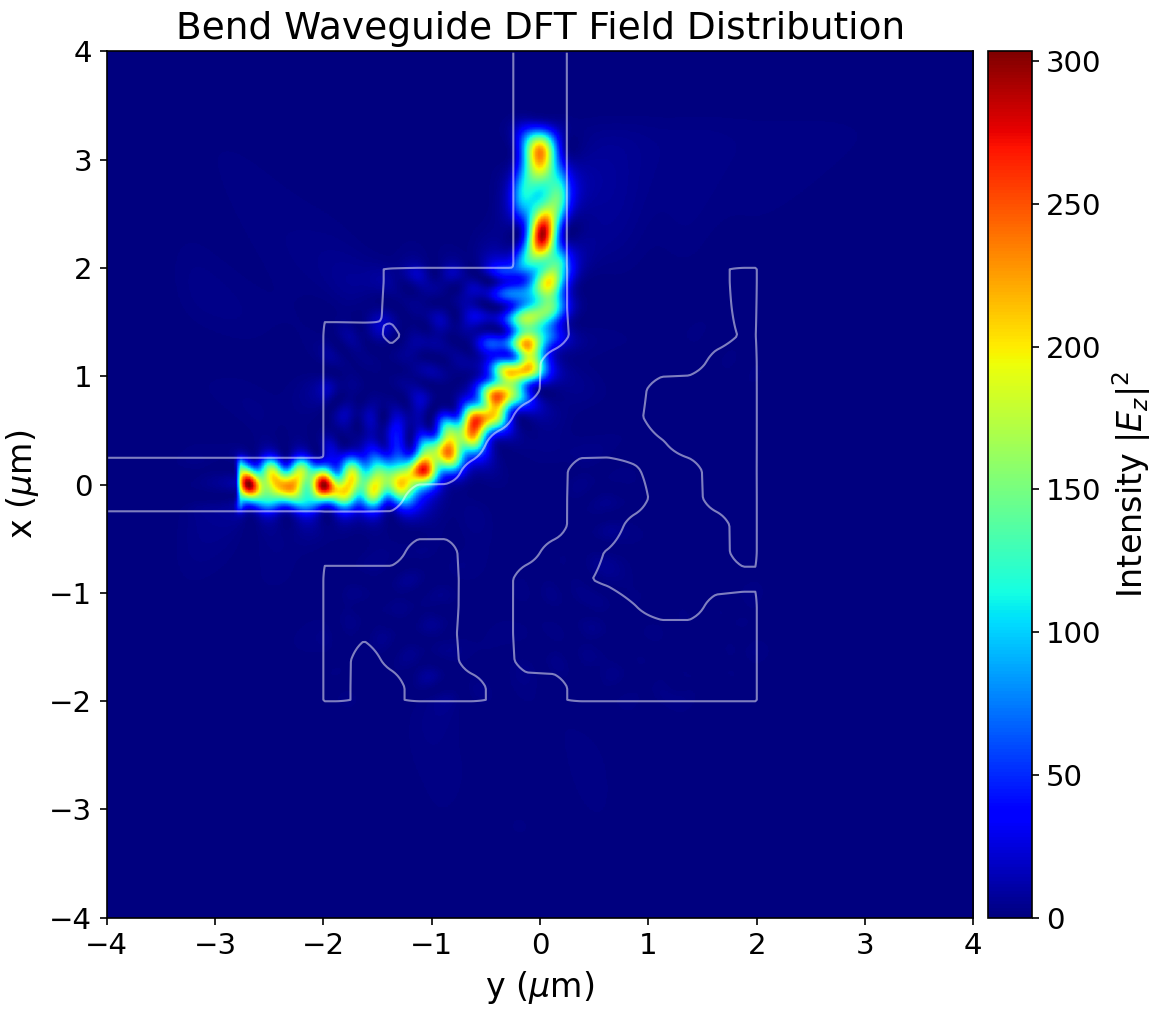
\includegraphics[width=0.8\textwidth]{img/BEND/BEND-GU-design4/eval_TE0_field.png}
\caption{彎曲波導 Design 4之DFT電場強度分布圖。}
\label{fig:BEND_DFT_design4}
\end{figure}

\begin{figure}[H]
\centering
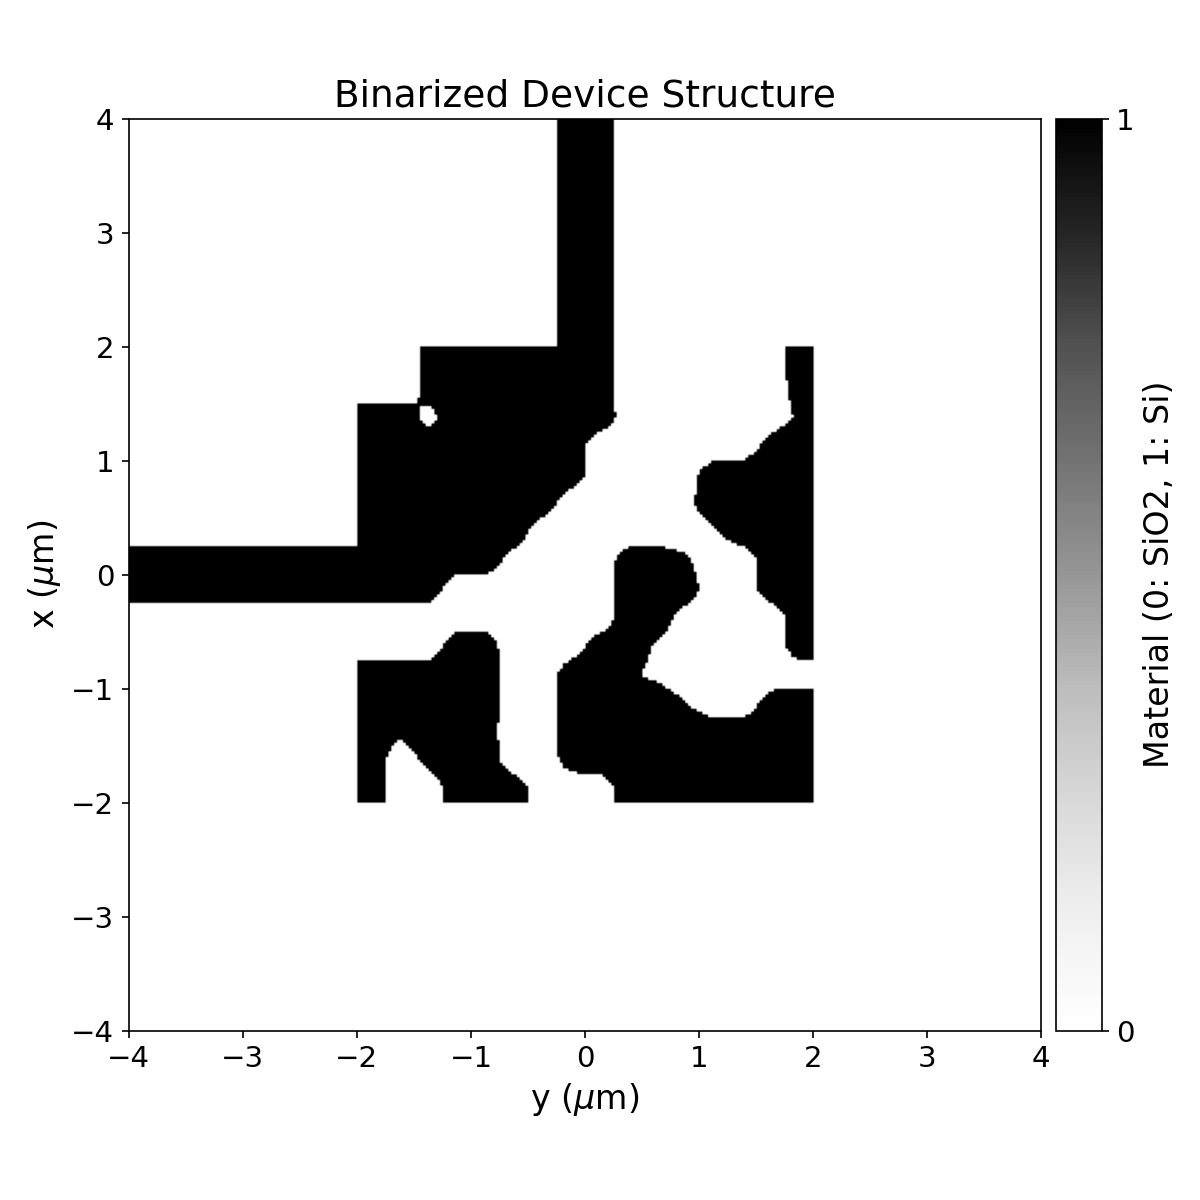
\includegraphics[width=0.7\textwidth]{img/BEND/BEND-GU-design4/eval_TE0_structure_binary.png}
\caption{彎曲波導 Design 4之幾何結構圖。}
\label{fig:BEND_structure_design4}
\end{figure}

\subsubsection{Gaussian Upsampling on Bend Waveguide Design - parameter 5}
最後，將設計網格進一步提升至 $20 \times 20$，為本研究中最高的維度，來評估在固定最佳化流程與資料量下，
持續增加設計自由度是否仍然能夠有效提升彎曲波導的最佳化表現。由於本實驗僅調整設計網格劃分設定，其餘模擬與最佳化設定皆維持與前述實驗一致，
以作為不同網格劃分之比較依據。

此實驗的最佳品質因數FoM為:
\begin{align}
FOM = 0.8281
\label{eq:BEND_FoM_Design5}
\end{align}
最終穿透率下降至82.81\%，較前兩組設計(\eqref{eq:BEND_FoM_Design3}與\eqref{eq:BEND_FoM_Design4})有更加的明顯下降，
表示持續增加設計的自由度並不能夠提升彎曲波導的傳輸效率。

由圖~\ref{fig:BEND_design5_Bestfom_vs_iteration}與圖~\ref{fig:BEND_design5_Opt_Trajactory}可觀察20×20設計之最佳化過程。
雖然候選解的最高FoM值依然隨著迭代次數增加而提升，但整體改善幅度相較於前面的設計明顯降低。
最佳FoM於初期提升至約0.72後，經過長時間搜尋才於後期進一步提升，最終收斂至0.8281。

此結果顯示，持續增加設計網格無法帶來更佳的傳輸效率，反而使最佳化過程需要更長的搜尋時間才能獲得有限改善。
由於$20 \times 20$設計具有較高的結構自由度，額外增加的設計變數並未有效轉換為性能提升，表示在本研究的資料量與最佳化架構下，過高的設計維度可能降低搜尋效率。
\begin{figure}[H]
\centering
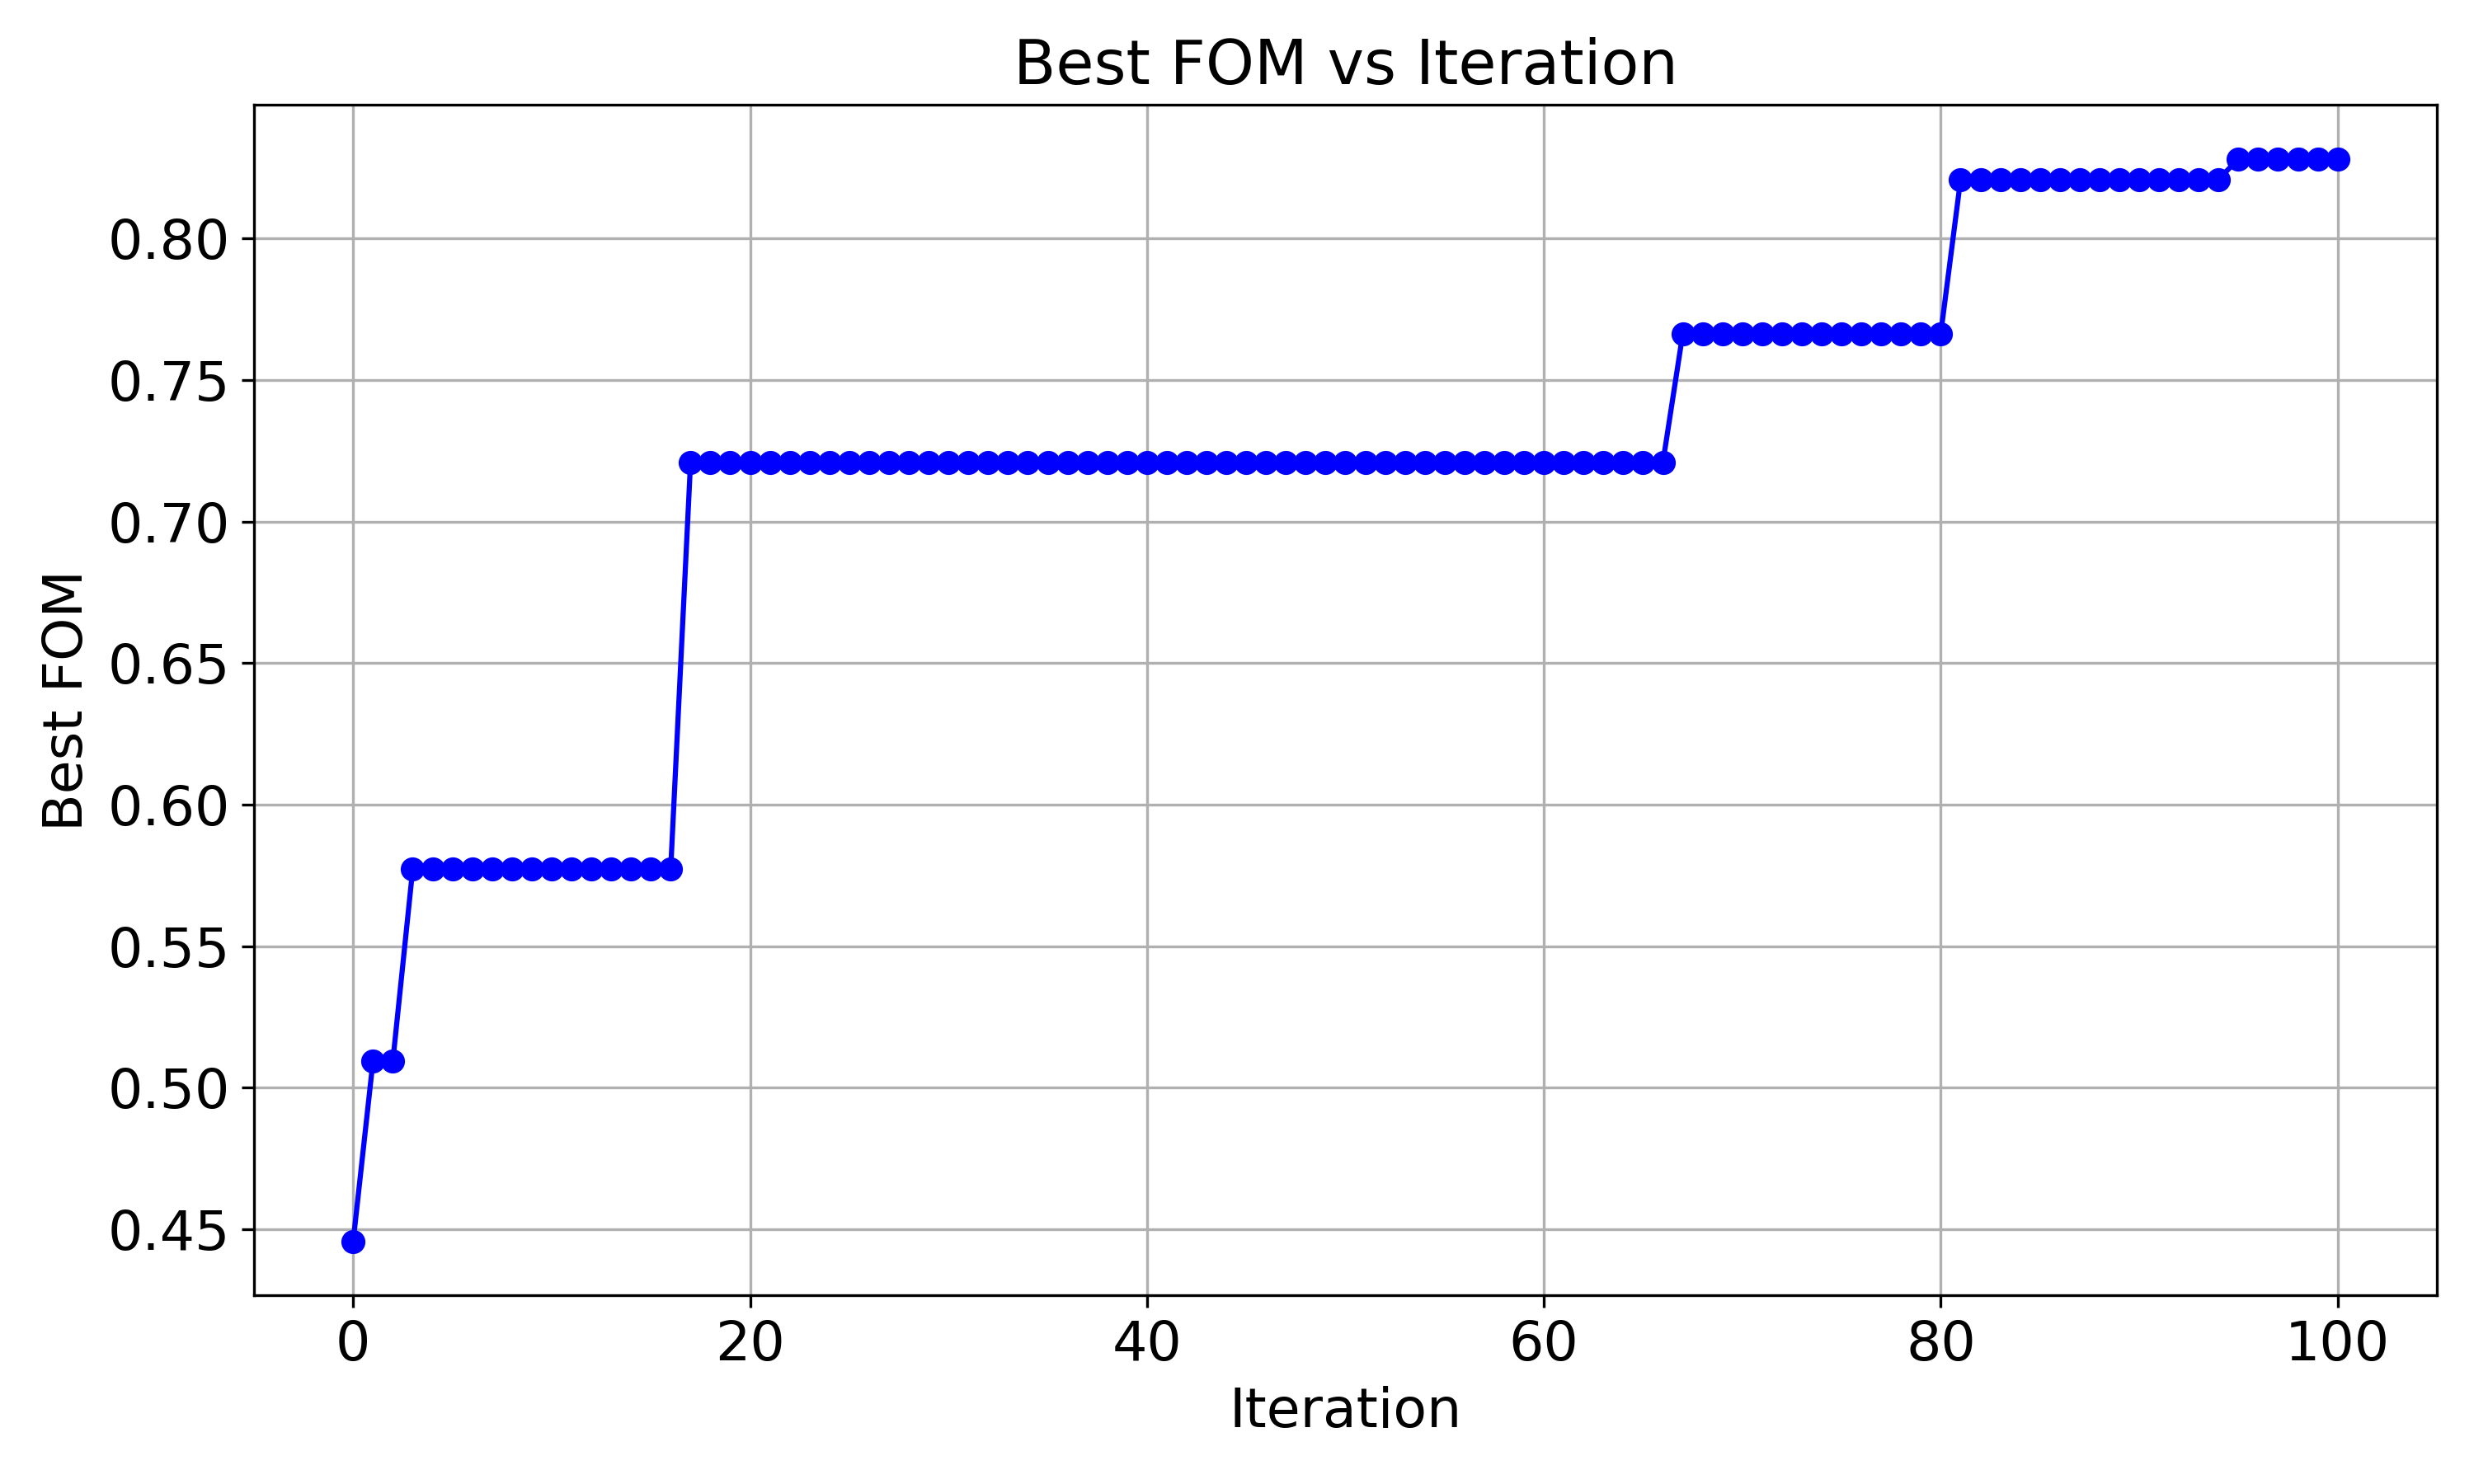
\includegraphics[width=0.8\textwidth]{img/BEND/BEND-GU-design5/fom_evolution.png}
\caption{彎曲波導 Design 5最佳化過程中的最佳FoM變化。}
\label{fig:BEND_design5_Bestfom_vs_iteration}
\end{figure}

\begin{figure}[H]
\centering
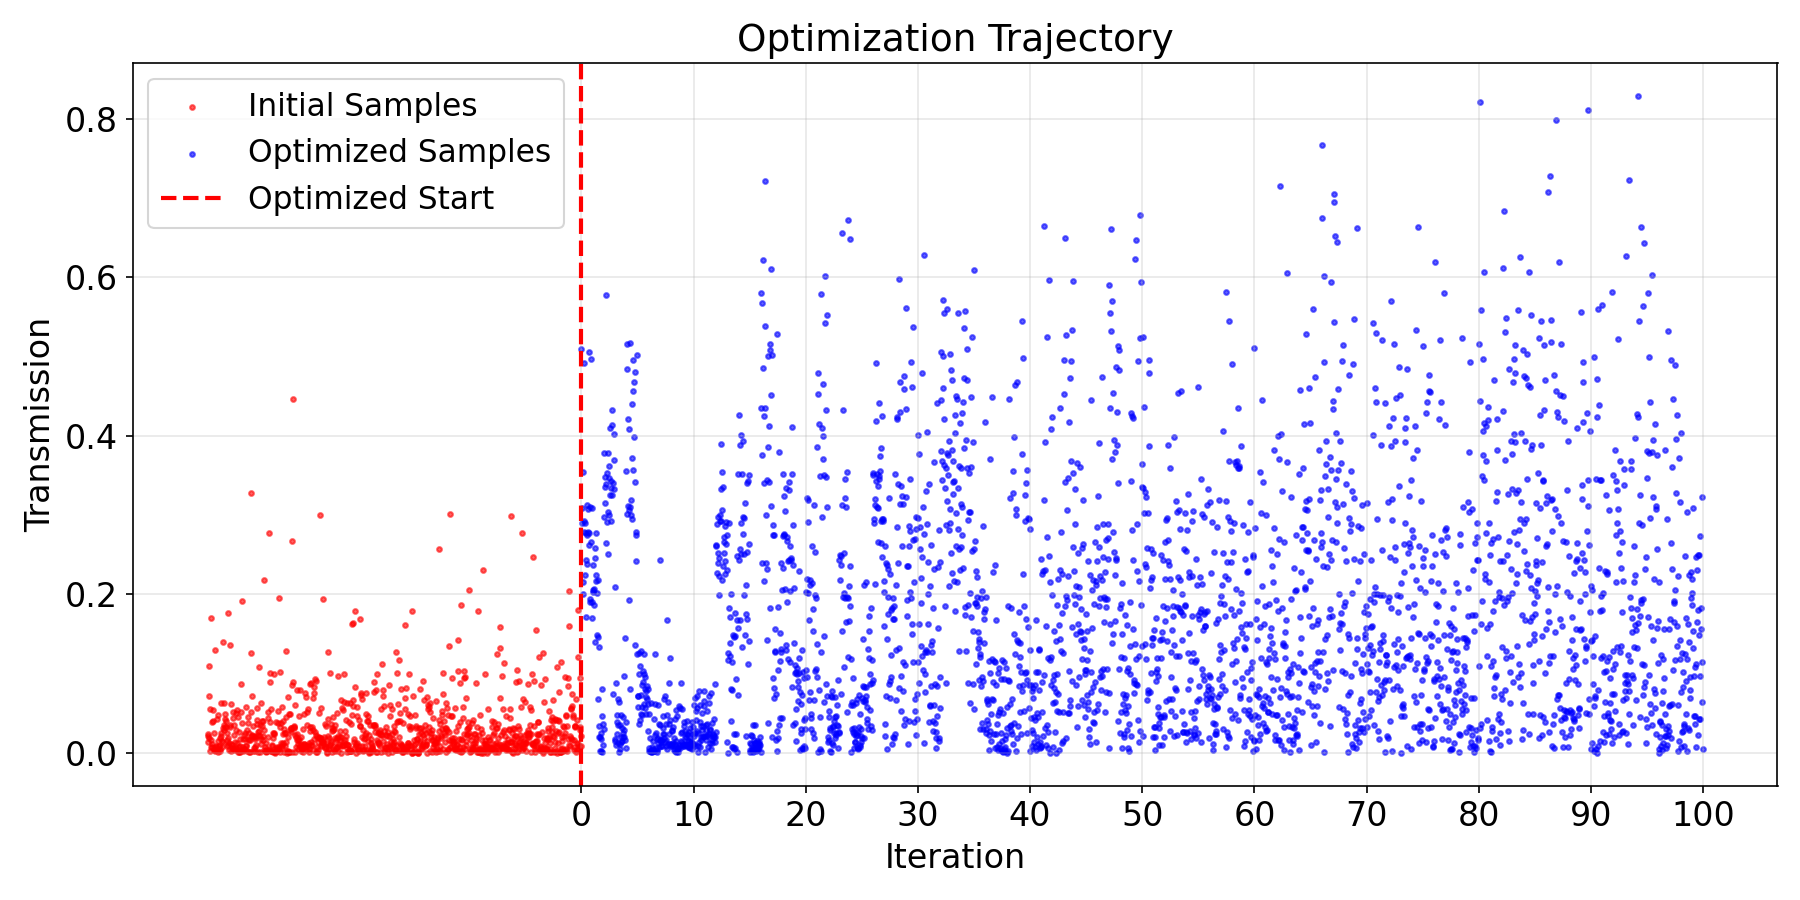
\includegraphics[width=0.8\textwidth]{img/BEND/BEND-GU-design5/transmission_trajectory.png}
\caption{彎曲波導 Design 5最佳化過程中的FoM變化。}
\label{fig:BEND_design5_Opt_Trajactory}
\end{figure}

圖~\ref{fig:BEND_DFT_design5}呈現$20 \times 20$設計並模擬的電場強度($|E_z|^2$)分布。由圖中可觀察到，
光波仍然能夠沿著彎曲波導傳輸至輸出端，並沒有出現明顯的漏光現象，但相較於前面的設計，在輸出端的模態分布有些微的不完整，
造成整體穿透率無法進一步提升。
\begin{figure}[H]
\centering
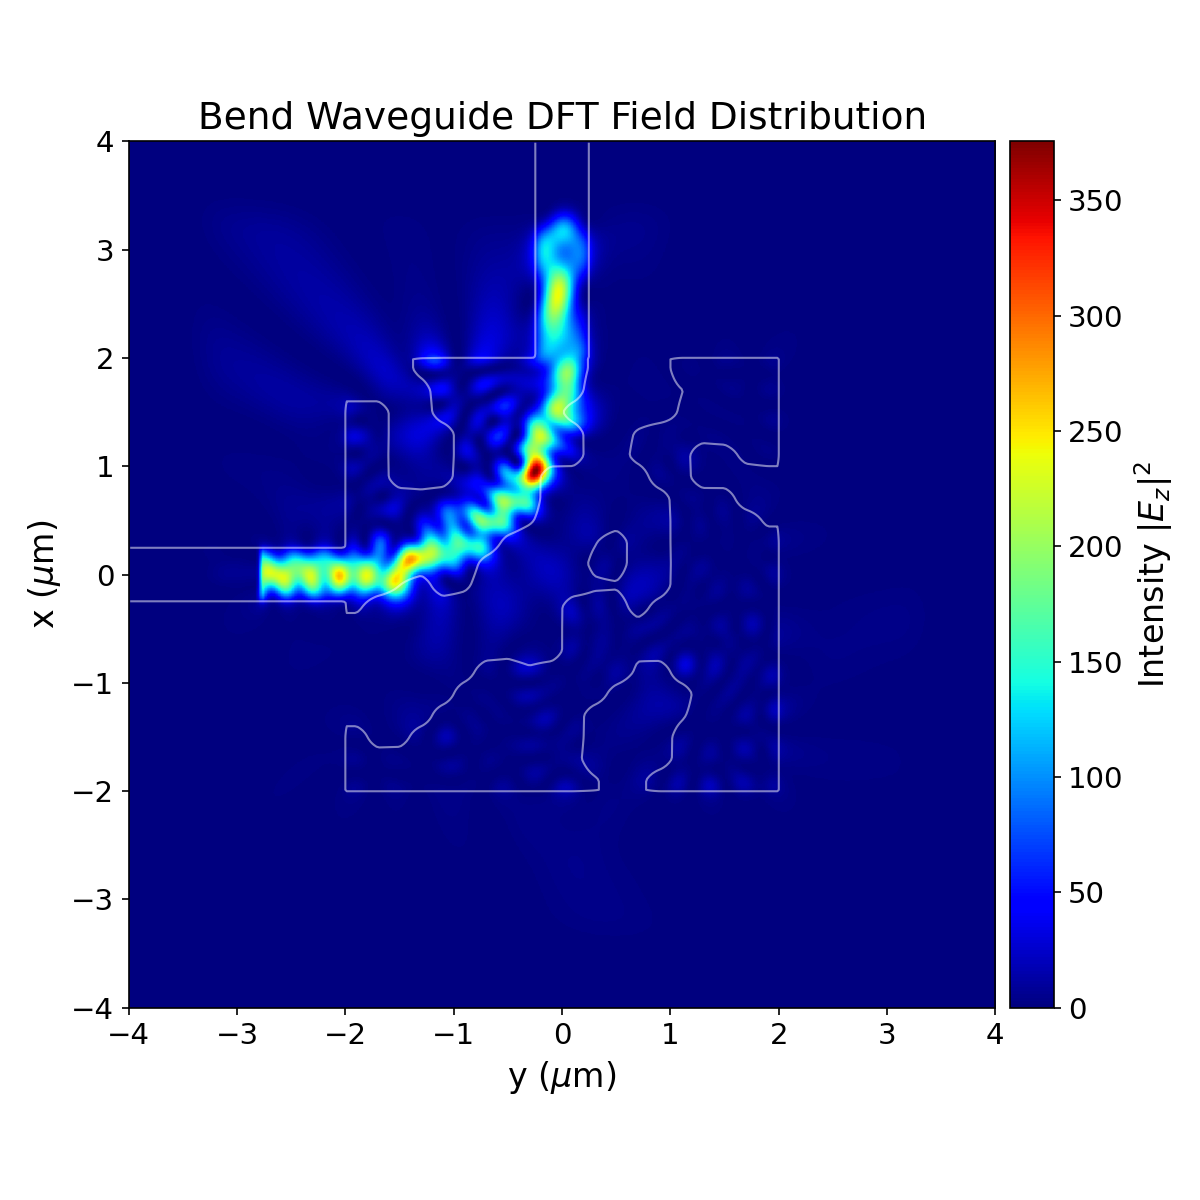
\includegraphics[width=0.8\textwidth]{img/BEND/BEND-GU-design5/eval_TE0_field.png}
\caption{彎曲波導 Design 5之DFT電場強度分布圖。}
\label{fig:BEND_DFT_design5}
\end{figure}
由圖~\ref{fig:BEND_structure_design5}可以觀察到，較高維度的設計網格能夠使結構具有更高的自由度，
並產生較多局部化的結構以及非連續區域，但這些額外的幾何結構變化並不能夠帶來更好的光場傳輸效率，
進而導致最終穿透率反而低於$12 \times 12$與$16 \times 16$的設計。
\begin{figure}[H]
\centering
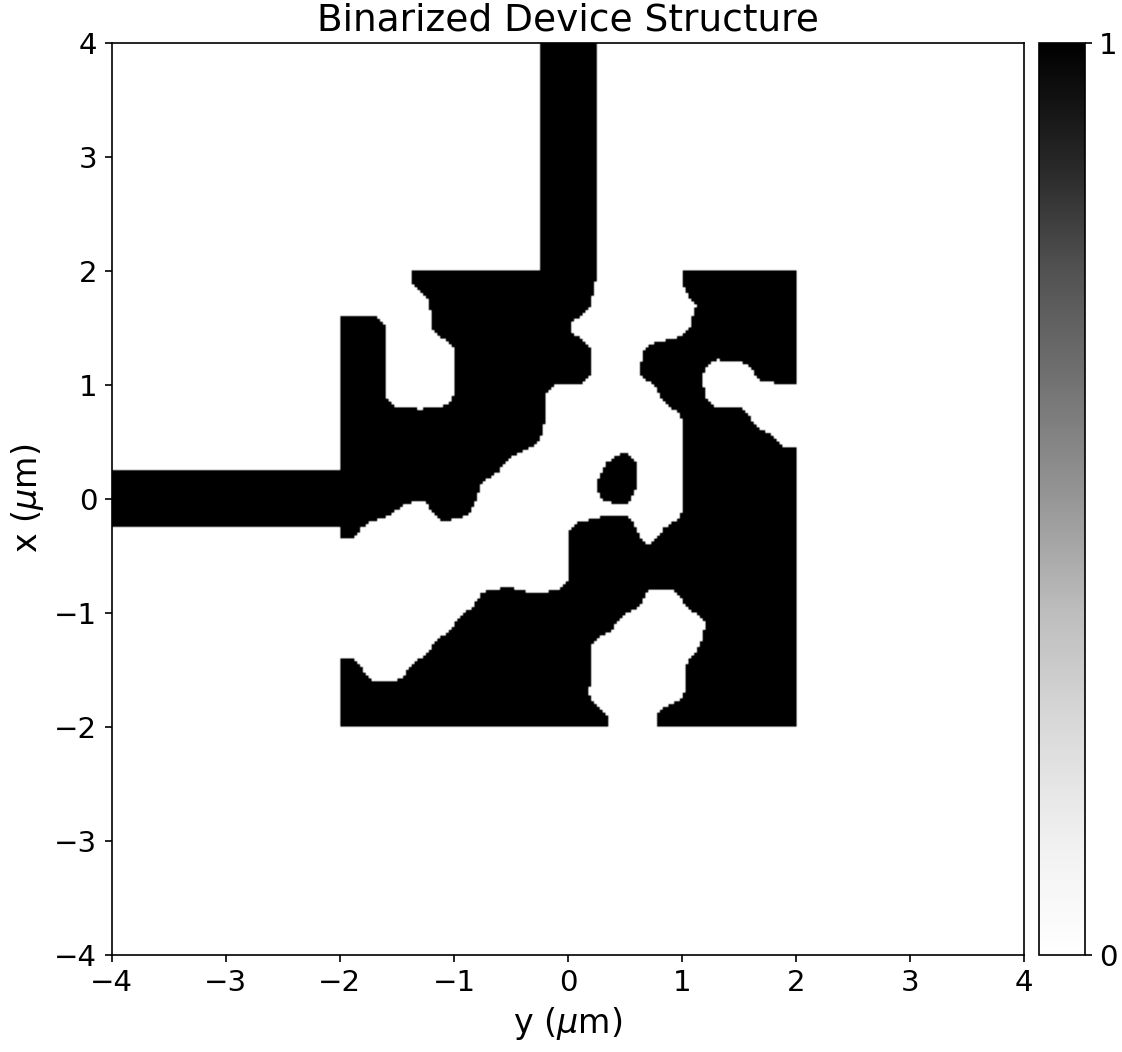
\includegraphics[width=0.7\textwidth]{img/BEND/BEND-GU-design5/eval_TE0_structure_binary.png}
\caption{彎曲波導 Design 5之幾何結構圖。}
\label{fig:BEND_structure_design5}
\end{figure}

\subsection{2D Fourier Integral on Bend Waveguide Design}
本節將會採用二維傅立葉積分(2D Fourier Integral)策略作為彎曲波導的結構編碼與平滑化設計方法，探討其於彎曲波導反向設計的最佳化潛力。

為了探討不同頻域設計自由度對於此最佳化策略結果的影響，本研究分別採用 $8\times8$、$10\times10$、$12\times12$、$16\times16$ 與 $20\times20$ 之頻譜空間變數進行實驗。
除了頻譜空間變數外，其餘 MEEP 模擬參數與最佳化流程皆維持一致，以確保不同設計維度間之比較具有一致性。

\subsubsection{2D Fourier Integral on Bend Waveguide Design - parameter 1}
\label{ch:2F_BEND_Design1}
首先，採用 $8 \times 8$ 之頻譜空間變數進行實驗，在模擬設定方面，MEEP 設計區域大小設為 $4.0 \times 4.0~\mu$m，
空間解析度(Resolution)設為 40 pixels/$\mu$m，輸入與輸出波導長度皆為 $1.0~\mu$m，波導寬度為 $0.5~\mu$m，並以 TE$_0$ 作為輸入模態。
光源採用 EigenModeSource 搭配 Gaussian Source 激發波長為$1550~$nm的 TE$_0$ 模態，以評估彎曲波導的傳輸效率。

在最佳化設定方面，初始隨機資料集大小設為1000筆，演算法共執行100次迭代，每次迭代模擬退火將會採樣出30筆候選解，
因此最終將會完成4000筆結構的評估，並且以穿透率(Transmission)作為品質因數(Figure of Merit, FoM)進行最佳化。

最終品質因數(FoM)為
\begin{align}
FOM = 0.9501
\label{eq:BEND_2F_design1_FOM}
\end{align}
由結果可知，採用 $8\times8$ 的頻譜空間變數即可獲得95.01\%的穿透率。

接著，可初步觀察最佳化過程中最佳FoM之演化，如圖~\ref{fig:BEND_2F_design1_Bestfom_vs_iteration}所示，最佳FoM會隨著迭代次數增加而逐漸提升，
表示FM模型結合模擬退火依然能夠持續找到具有較佳傳輸效率的候選解。此外，由圖~\ref{fig:BEND_2F_design1_Opt_Trajactory}可觀察到，
整體候選解之FoM分布也會隨著最佳化過程逐漸向高FoM區域移動，表示演算法具有良好的搜尋能力。
\begin{figure}[H]
\centering
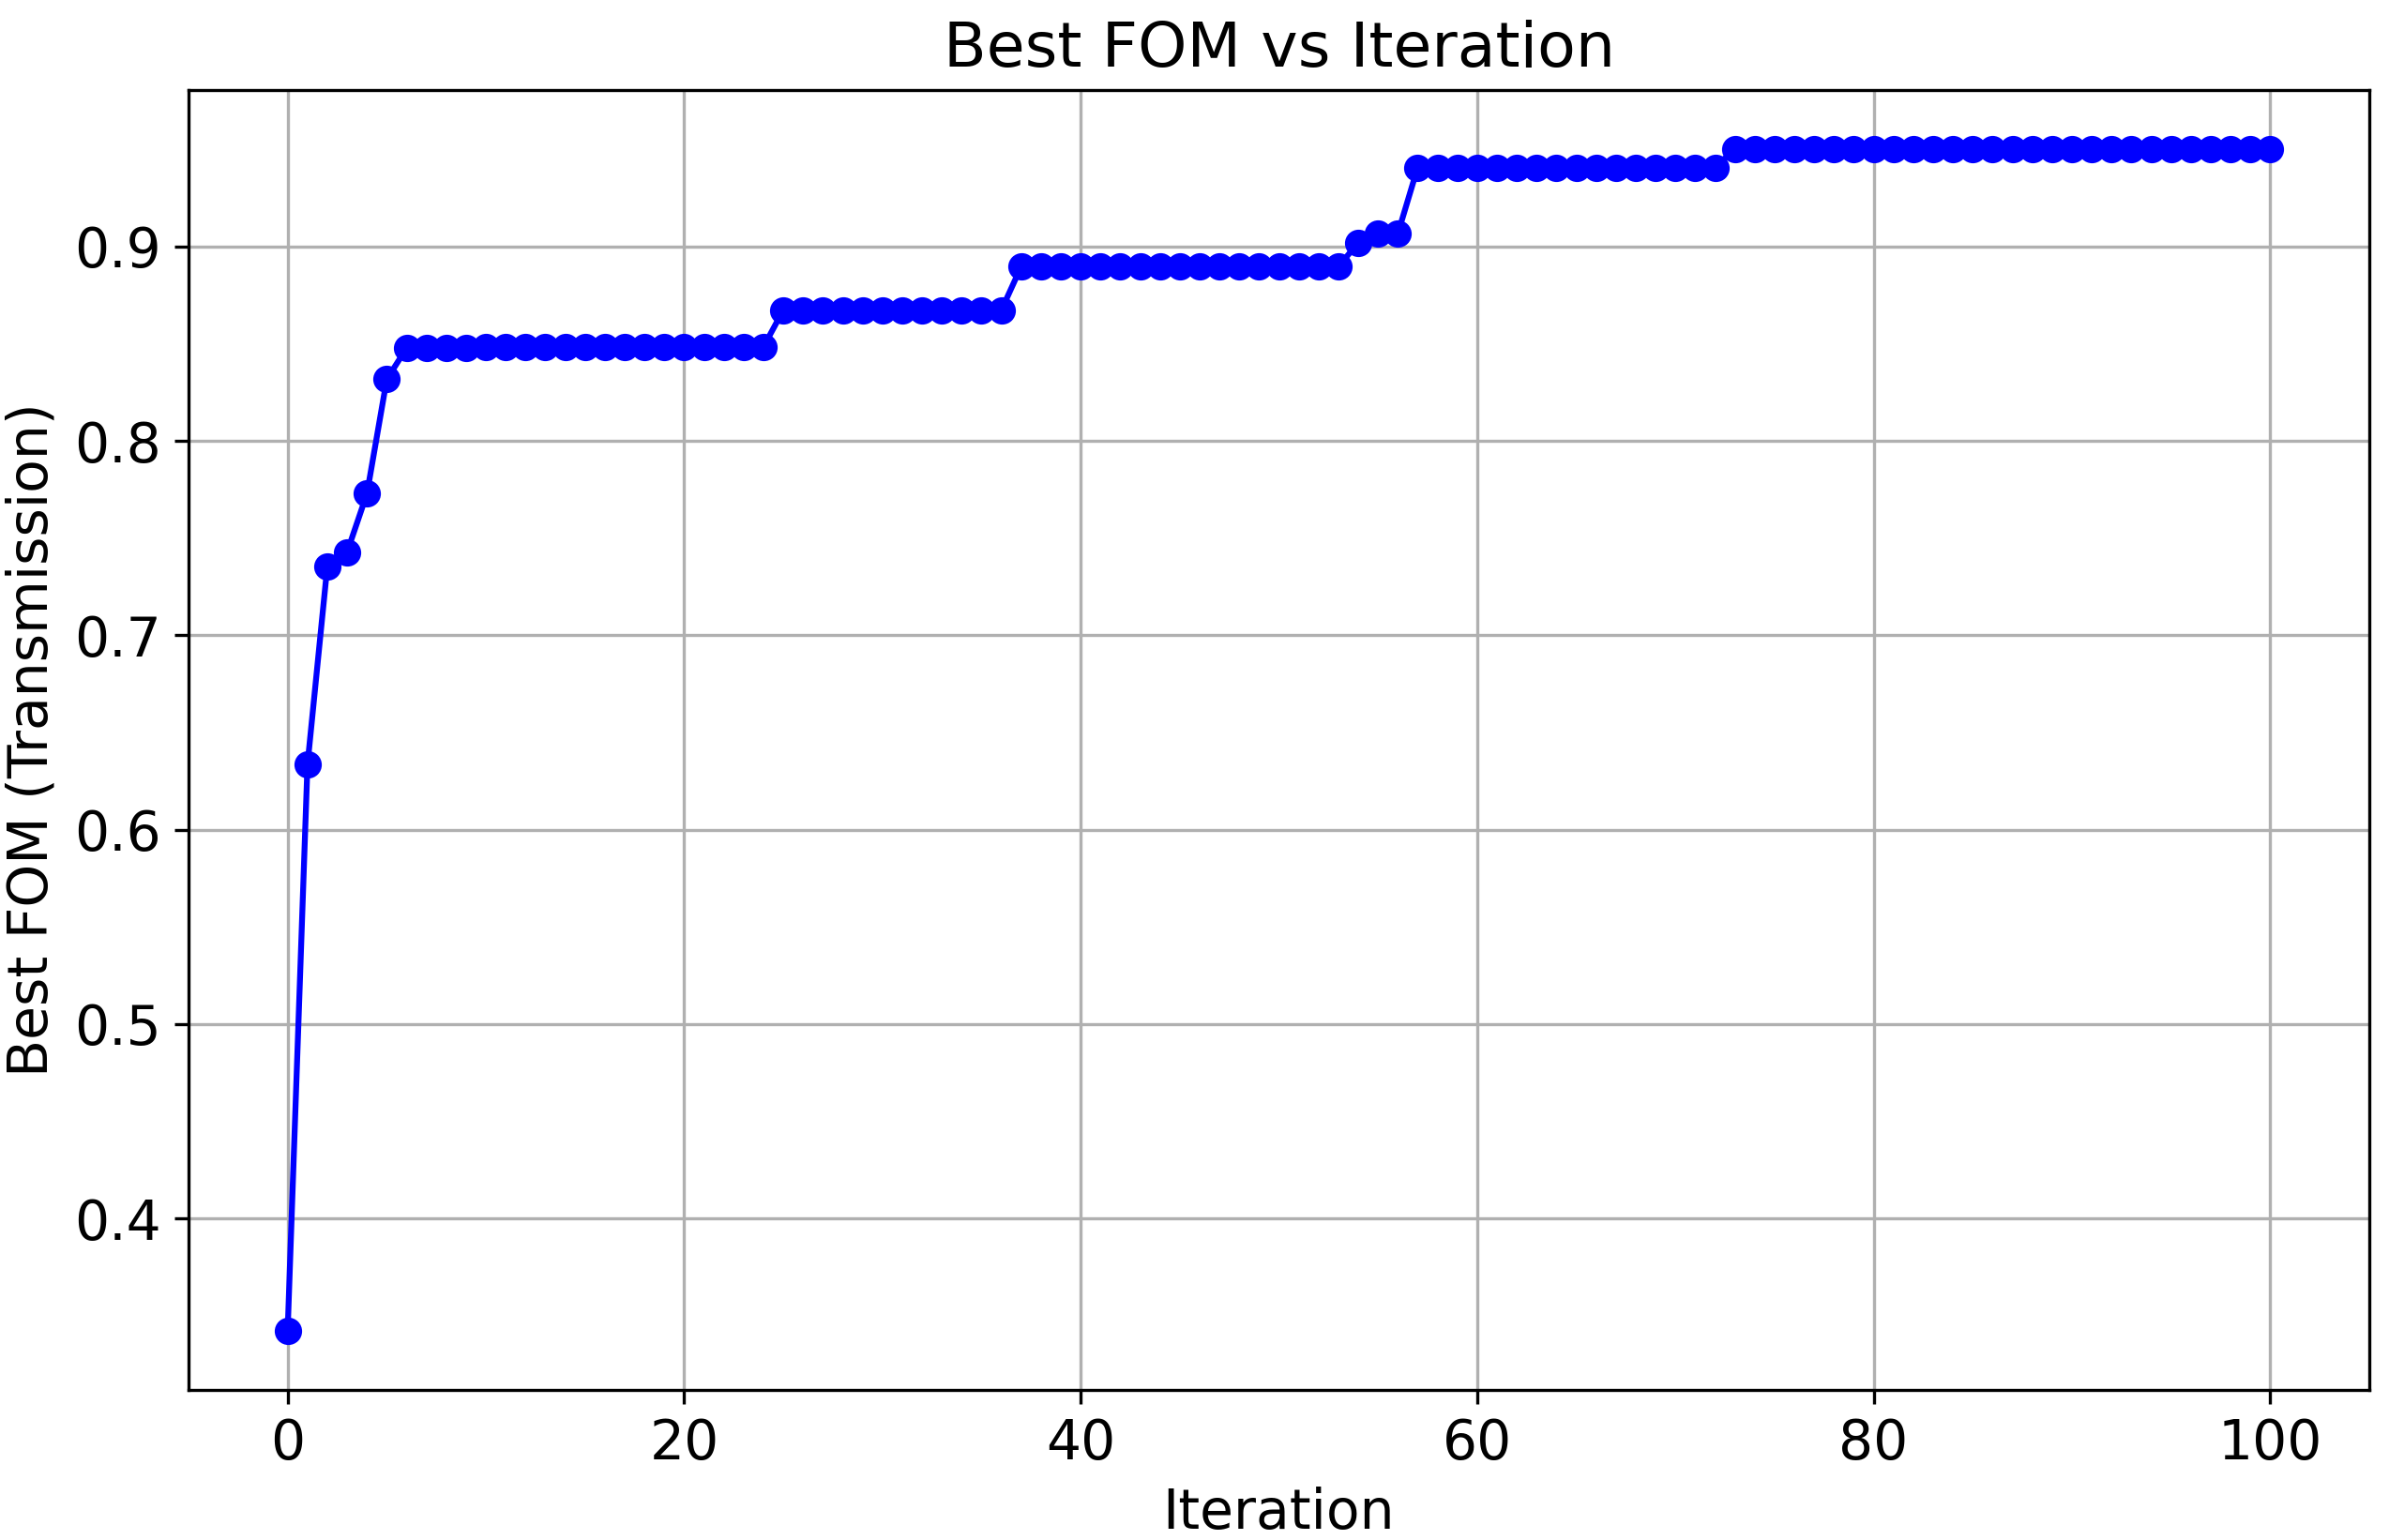
\includegraphics[width=0.9\textwidth]{img/BEND/BEND-2F-design1/fom_evolution.png}
\caption{二維傅立葉積分策略應用於彎曲波導 Design 1最佳化過程中的最佳FoM變化。}
\label{fig:BEND_2F_design1_Bestfom_vs_iteration}
\end{figure}

\begin{figure}[H]
\centering
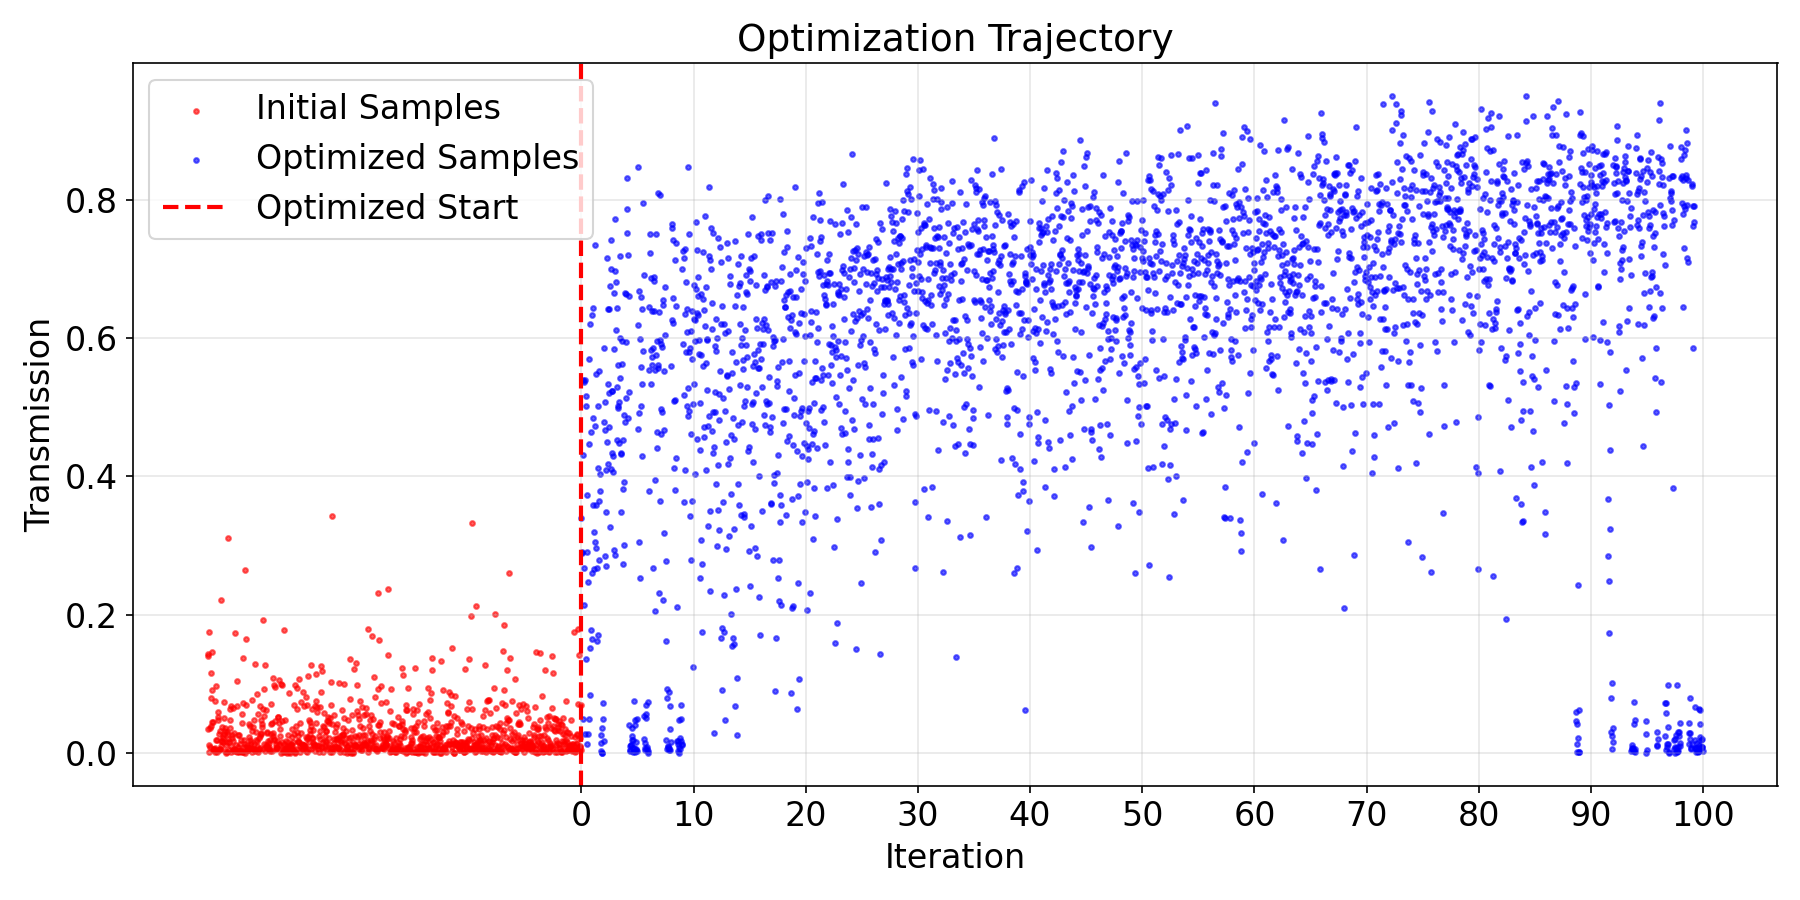
\includegraphics[width=1.0\textwidth]{img/BEND/BEND-2F-design1/transmission_trajectory.png}
\caption{二維傅立葉積分策略應用於彎曲波導 Design 1最佳化過程中的FoM變化。}
\label{fig:BEND_2F_design1_Opt_Trajactory}
\end{figure}

圖~\ref{fig:BEND_2F_DFT_design1}呈現二維傅立葉積分策略應用於彎曲波導 Design 1之電場強度（$|E_z|^2$）分布，
圖~\ref{fig:BEND_2F_structure_design1}呈現二維傅立葉積分策略應用於彎曲波導 Design 1之幾何結構圖。
由這兩張圖可以發現，最佳化後的結構在彎曲區域形成向內側偏移的幾何特徵，這個結果與傳統低損耗彎曲波導常見之設計趨勢一致，
有助於改善光場在彎曲處的傳輸特性，並且光波在通過彎曲區域後仍然能夠順利耦合至輸出波導，沒有出現明顯的漏光或反射現象，
顯示二維傅立葉積分策略所設計出的結構能夠具有良好的導光能力。
\begin{figure}[H]
\centering
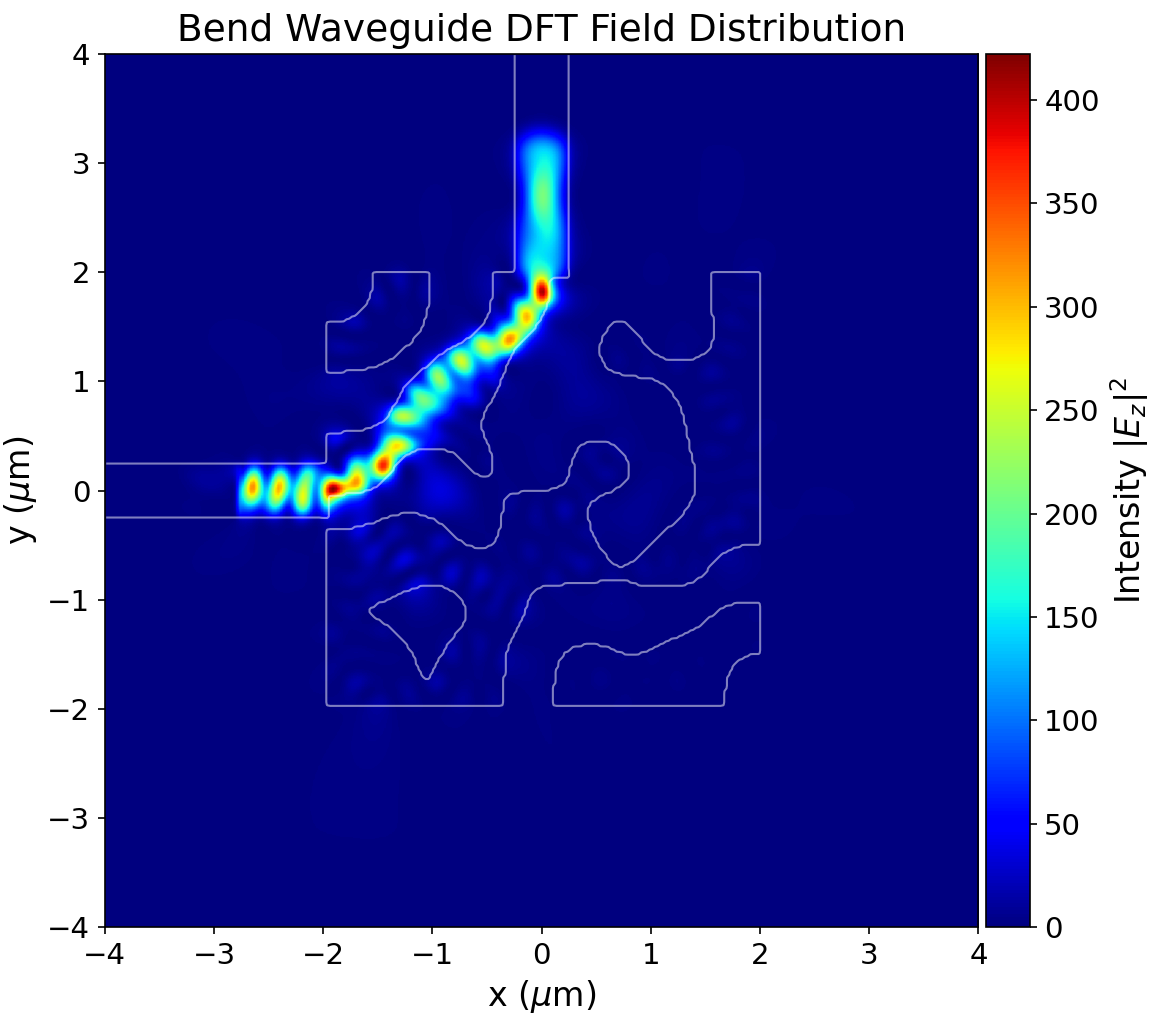
\includegraphics[width=0.8\textwidth]{img/BEND/BEND-2F-design1/final_analysis_TE0_field.png}
\caption{二維傅立葉積分策略應用於彎曲波導 Design 1之DFT電場強度分布圖。}
\label{fig:BEND_2F_DFT_design1}
\end{figure}

\begin{figure}[H]
\centering
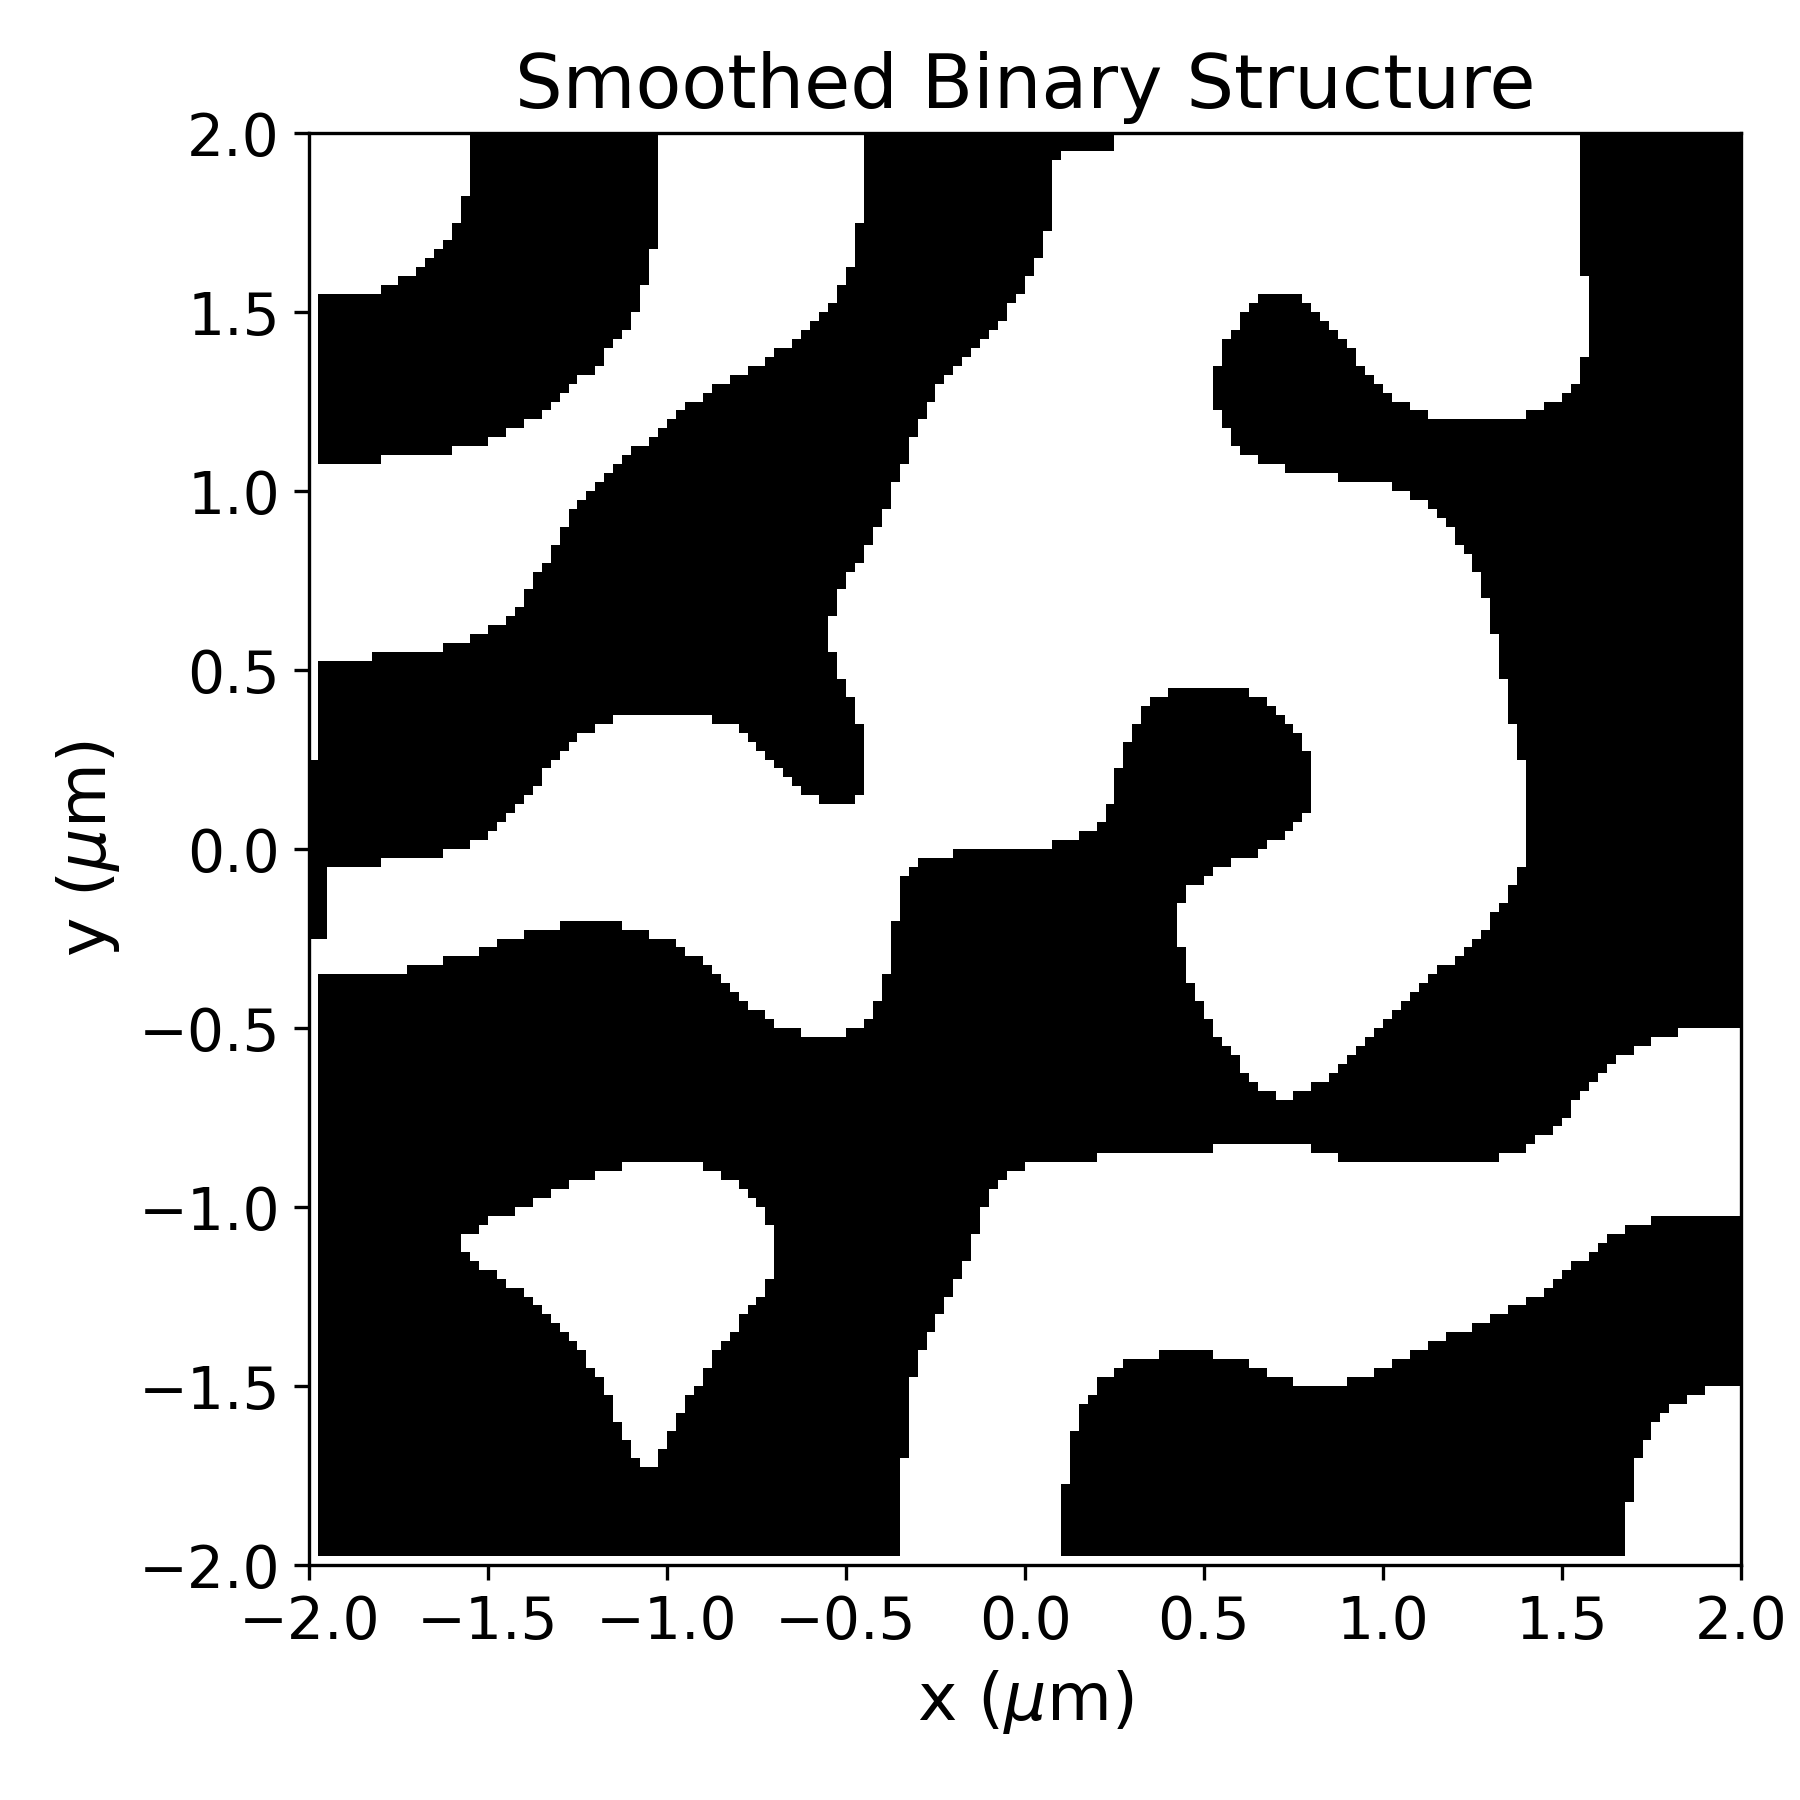
\includegraphics[width=0.7\textwidth]{img/BEND/BEND-2F-design1/Smoothed_Binary_Structure.png}
\caption{二維傅立葉積分策略應用於彎曲波導 Design 1之幾何結構圖。}
\label{fig:BEND_2F_structure_design1}
\end{figure}

\subsubsection{2D Fourier Integral on Bend Waveguide Design - parameter 2}
\label{ch:2F_BEND_Design2}
接著，將頻譜空間變數由 $8\times8$ 提升至 $10\times10$，以探討適度增加設計自由度是否能進一步提升彎曲波導之最佳化效能。
除頻譜空間變數維度外，其餘 MEEP 模擬參數、光源設定及最佳化流程皆與 Design 1 (第~\ref{ch:2F_BEND_Design1}節)相同，以確保不同設計維度間具有一致之比較基準。

最終FoM提升至:
\begin{align}
FOM = 0.9930
\label{eq:BEND_2DF_design2_FOM}
\end{align}
採用 $10 \times 10$ 頻譜空間變數所設計的彎曲波導結構，最終穿透率達99.30\%，為本系列實驗中最佳的最佳化結果，或許適度增加設計自由度有助於提升彎曲波導的傳輸效能。

接著，觀察最佳化過程中的最佳FoM變化如圖~\ref{fig:BEND_2F_design2_Bestfom_vs_iteration}與圖~\ref{fig:BEND_2F_design2_Opt_Trajactory}所示，
相較於Design 1(第~\ref{ch:2F_BEND_Design1}節)，可以發現Design 2雖然沒有在初期迭代快速收斂，反而是在大約20次迭代前的樣本皆與初始訓練資料集相似，維持在FoM較低的區域，
但是整體FoM在大約25次迭代後FoM大幅上升，最後在約第95次迭代搜尋到了最佳解，達到99.30\%之穿透率。
\begin{figure}[H]
\centering
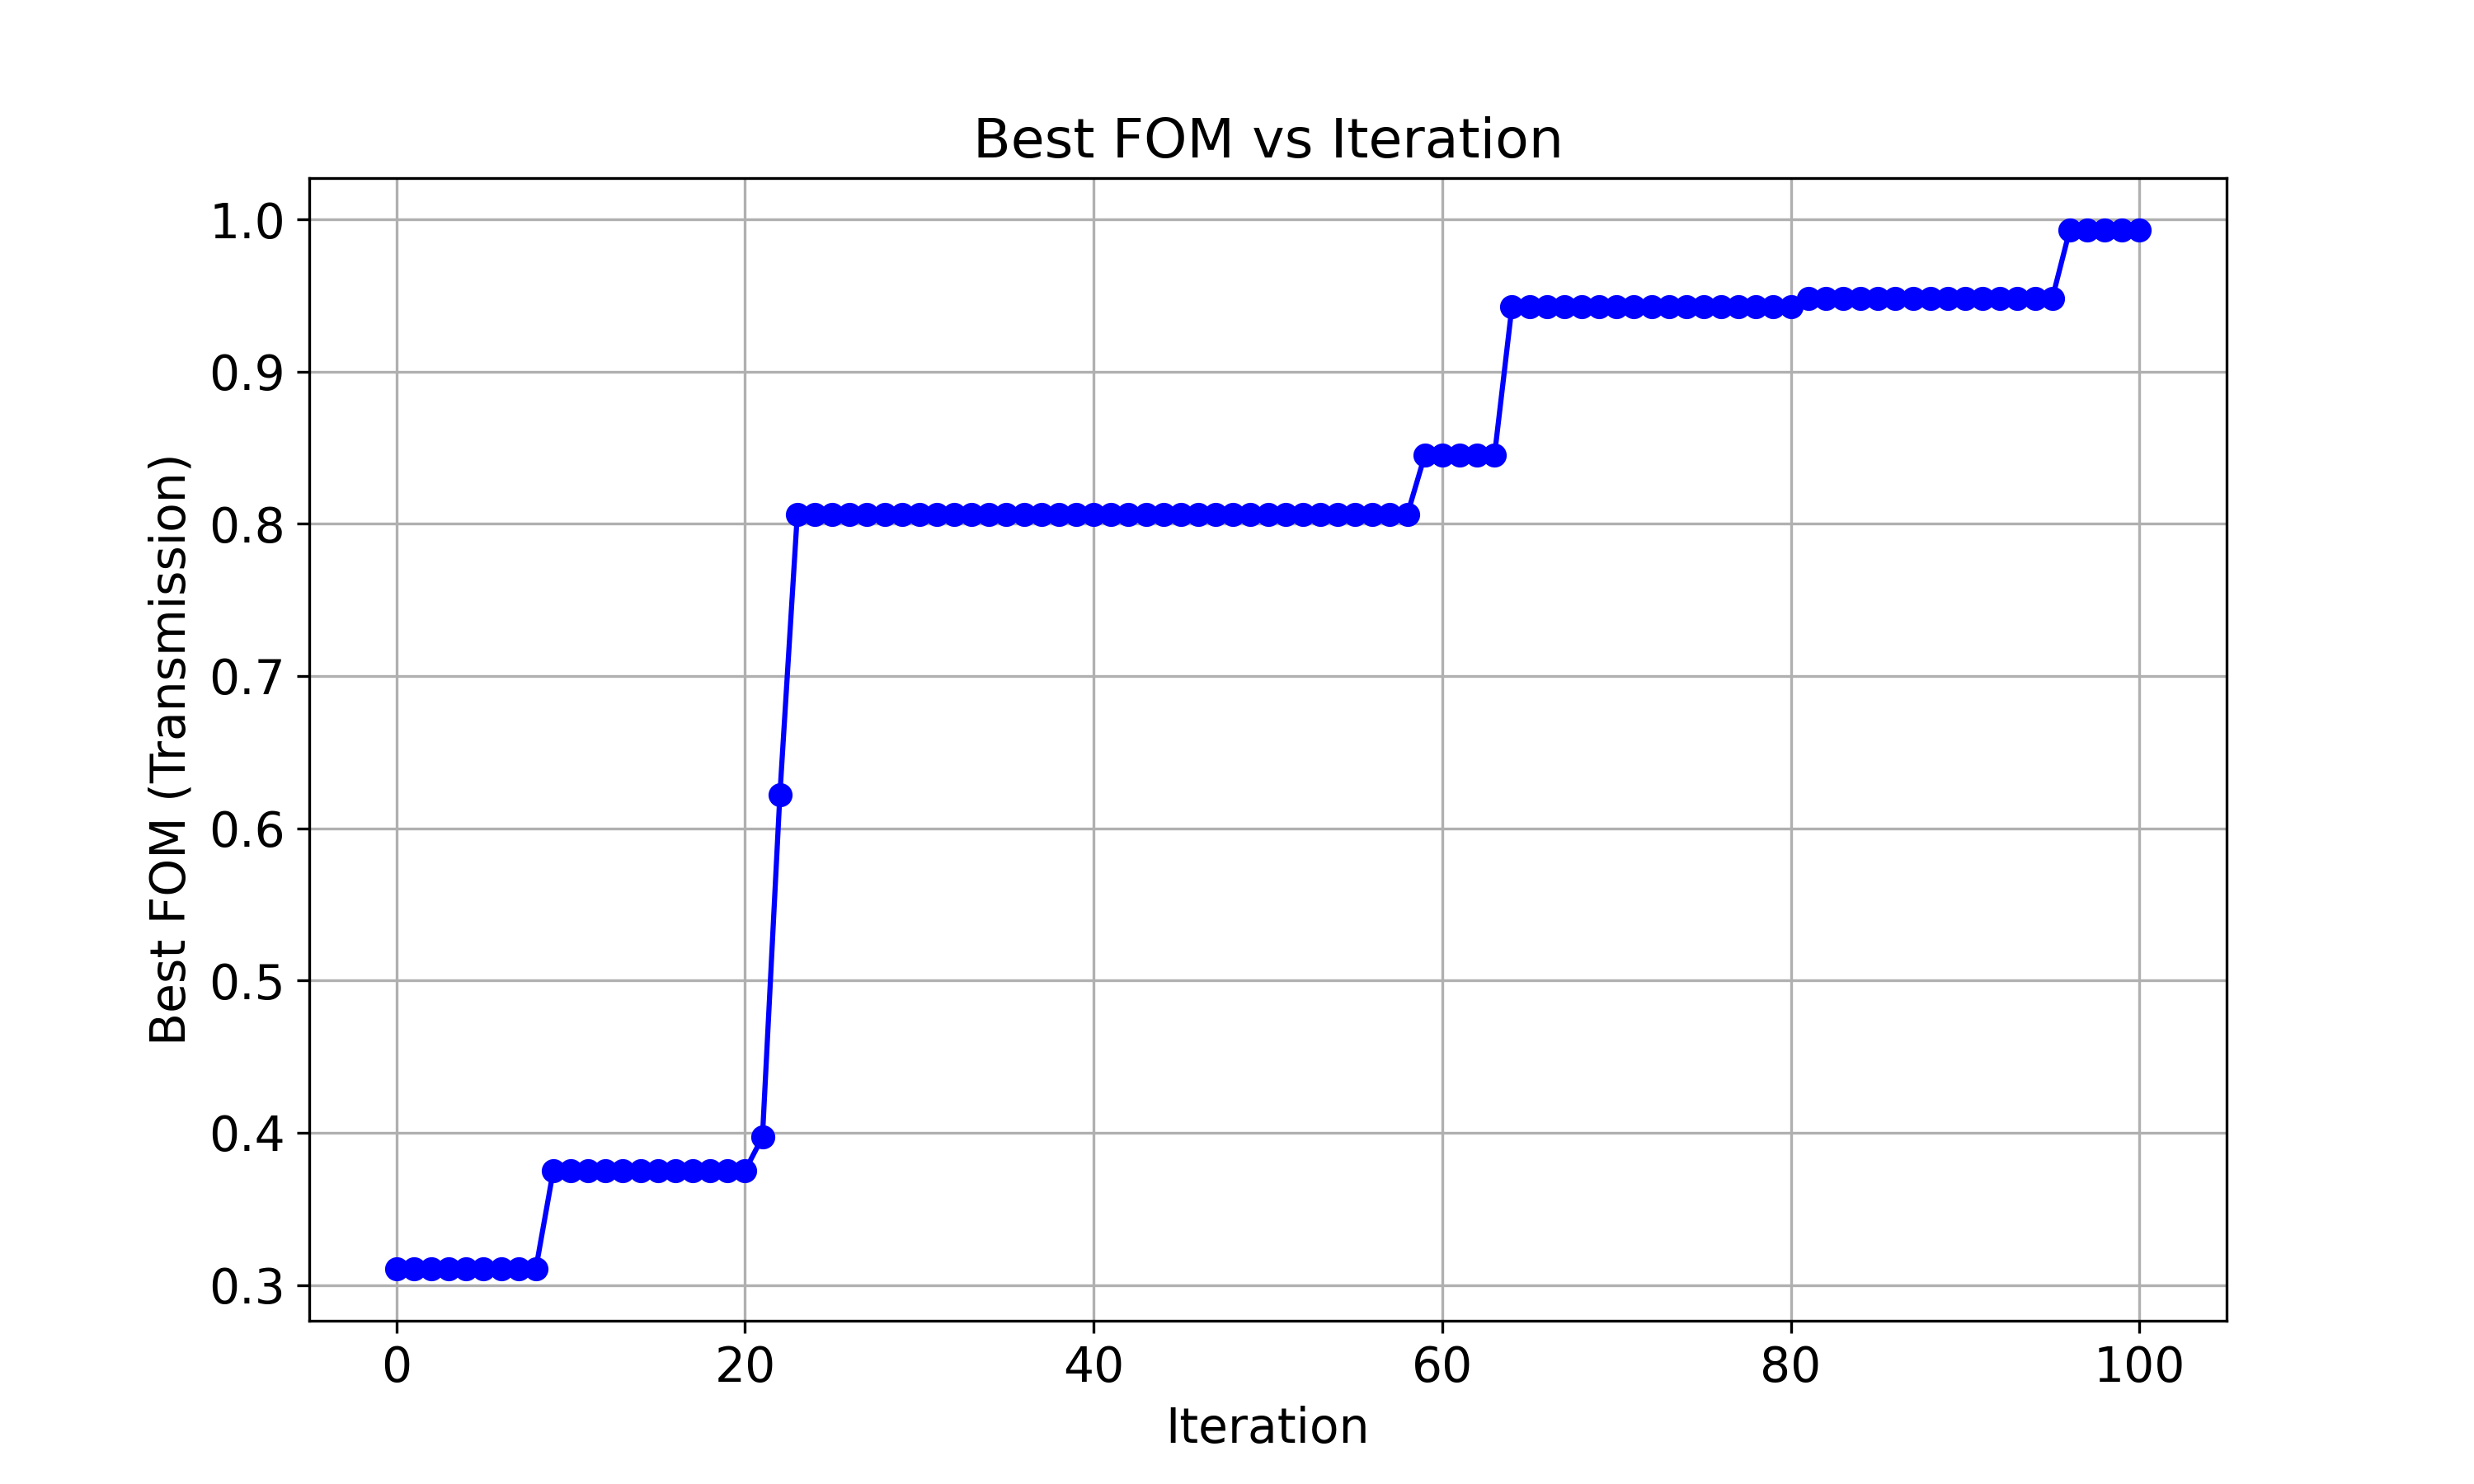
\includegraphics[width=0.9\textwidth]{img/BEND/BEND-2F-design2/fom_evolution.png}
\caption{二維傅立葉積分策略應用於彎曲波導 Design 2最佳化過程中的最佳FoM變化。}
\label{fig:BEND_2F_design2_Bestfom_vs_iteration}
\end{figure}

\begin{figure}[H]
\centering
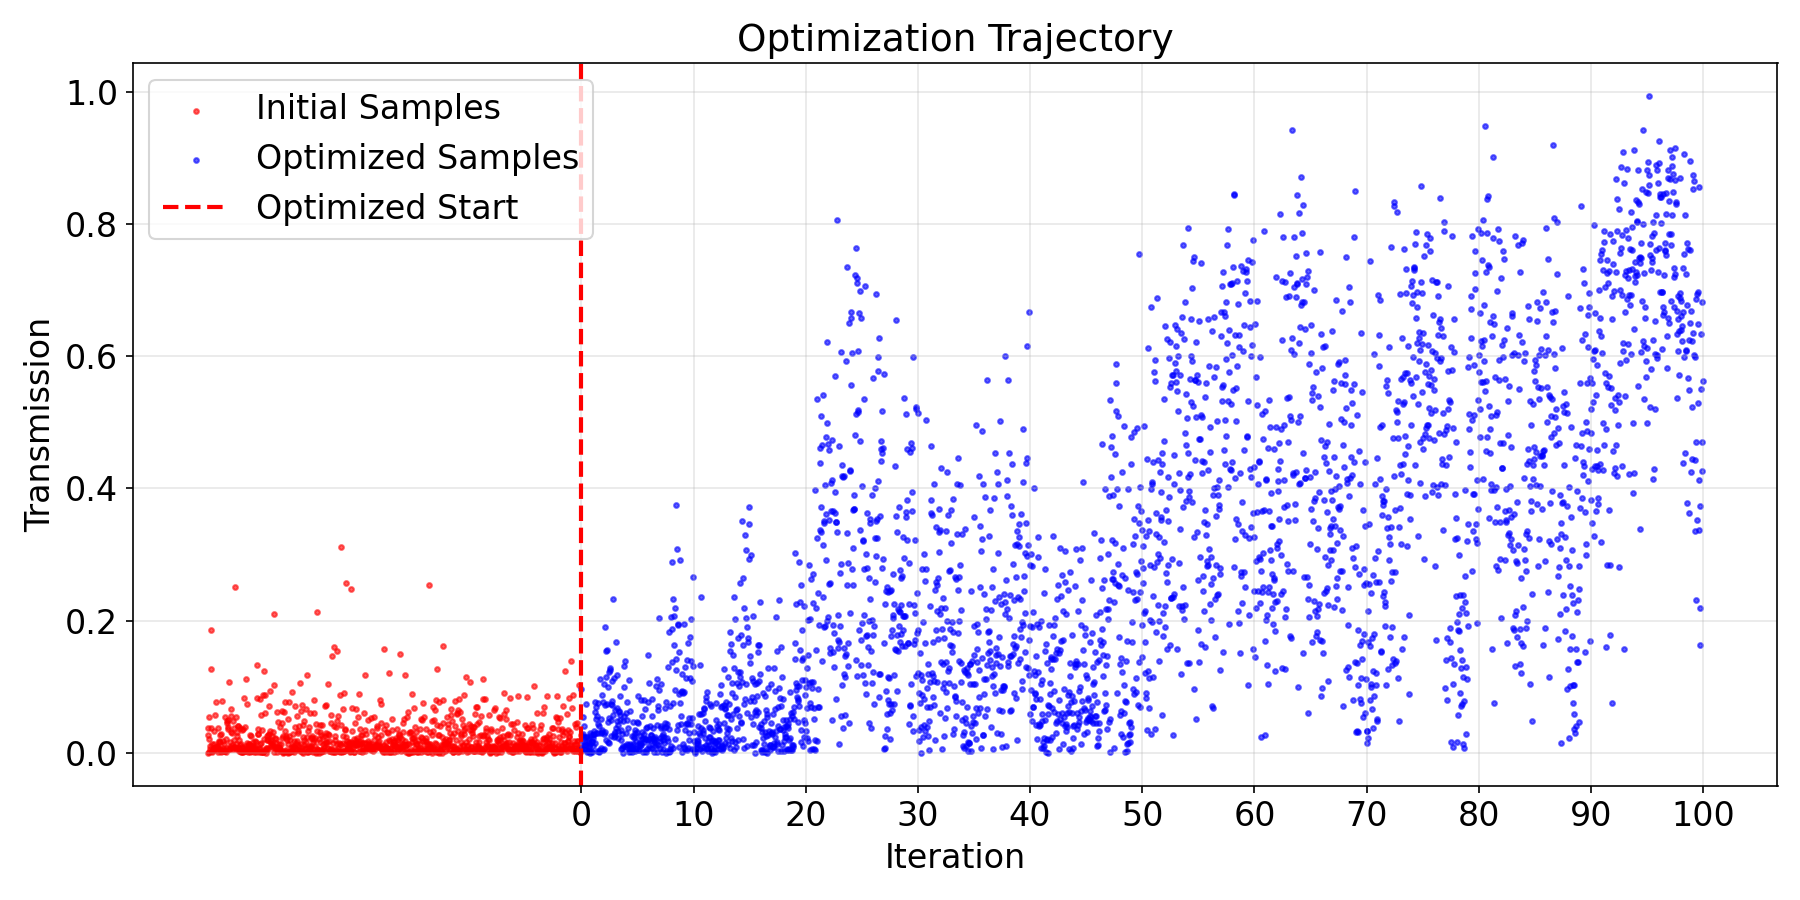
\includegraphics[width=1.0\textwidth]{img/BEND/BEND-2F-design2/transmission_trajectory.png}
\caption{二維傅立葉積分策略應用於彎曲波導 Design 2最佳化過程中的FoM變化。}
\label{fig:BEND_2F_design2_Opt_Trajactory}
\end{figure}
圖~\ref{fig:BEND_2F_DFT_design2}顯示光場在彎曲區域仍能維持穩定傳播，
通過彎曲段後快速耦合至輸出波導，整體光場分布相當完整，與99.30\%的高穿透率結果完全一致。
\begin{figure}[H]
\centering
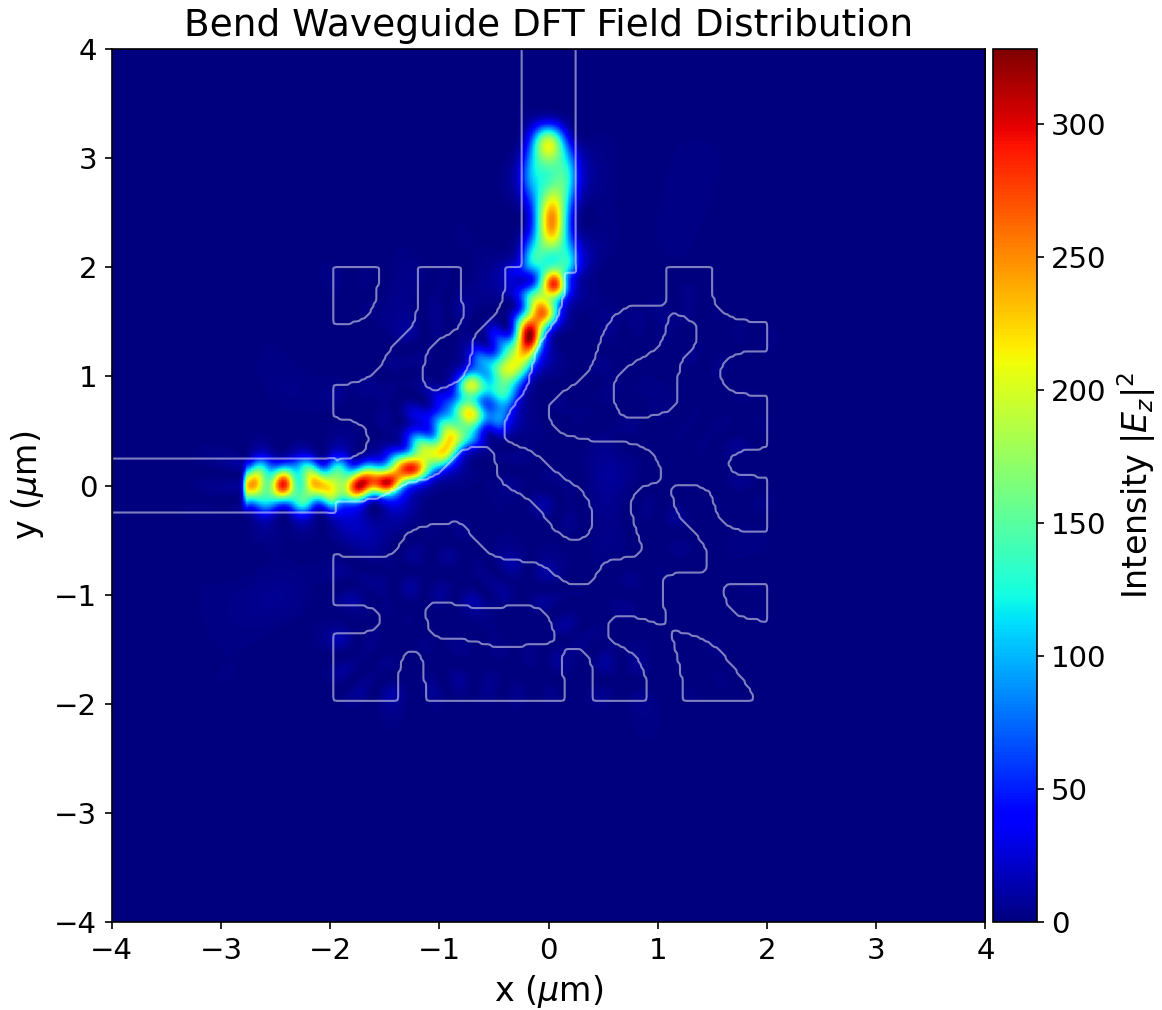
\includegraphics[width=0.8\textwidth]{img/BEND/BEND-2F-design2/final_analysis_TE0_field.png}
\caption{二維傅立葉積分策略應用於彎曲波導 Design 2之DFT電場強度分布圖。}
\label{fig:BEND_2F_DFT_design2}
\end{figure}
相較於 Design 1(第~\ref{ch:2F_BEND_Design1}節)，圖~\ref{fig:BEND_2F_structure_design2}可以觀察到同樣也有設計出類似內側偏移的結構，
增加至 $10\times10$ 頻譜空間變數後，最佳化結構能夠形成更多細部幾何特徵。然而，整體邊界仍維持平滑且連續，並沒有因為增加設計自由度而產生明顯的局部不連續現象。
\begin{figure}[H]
\centering
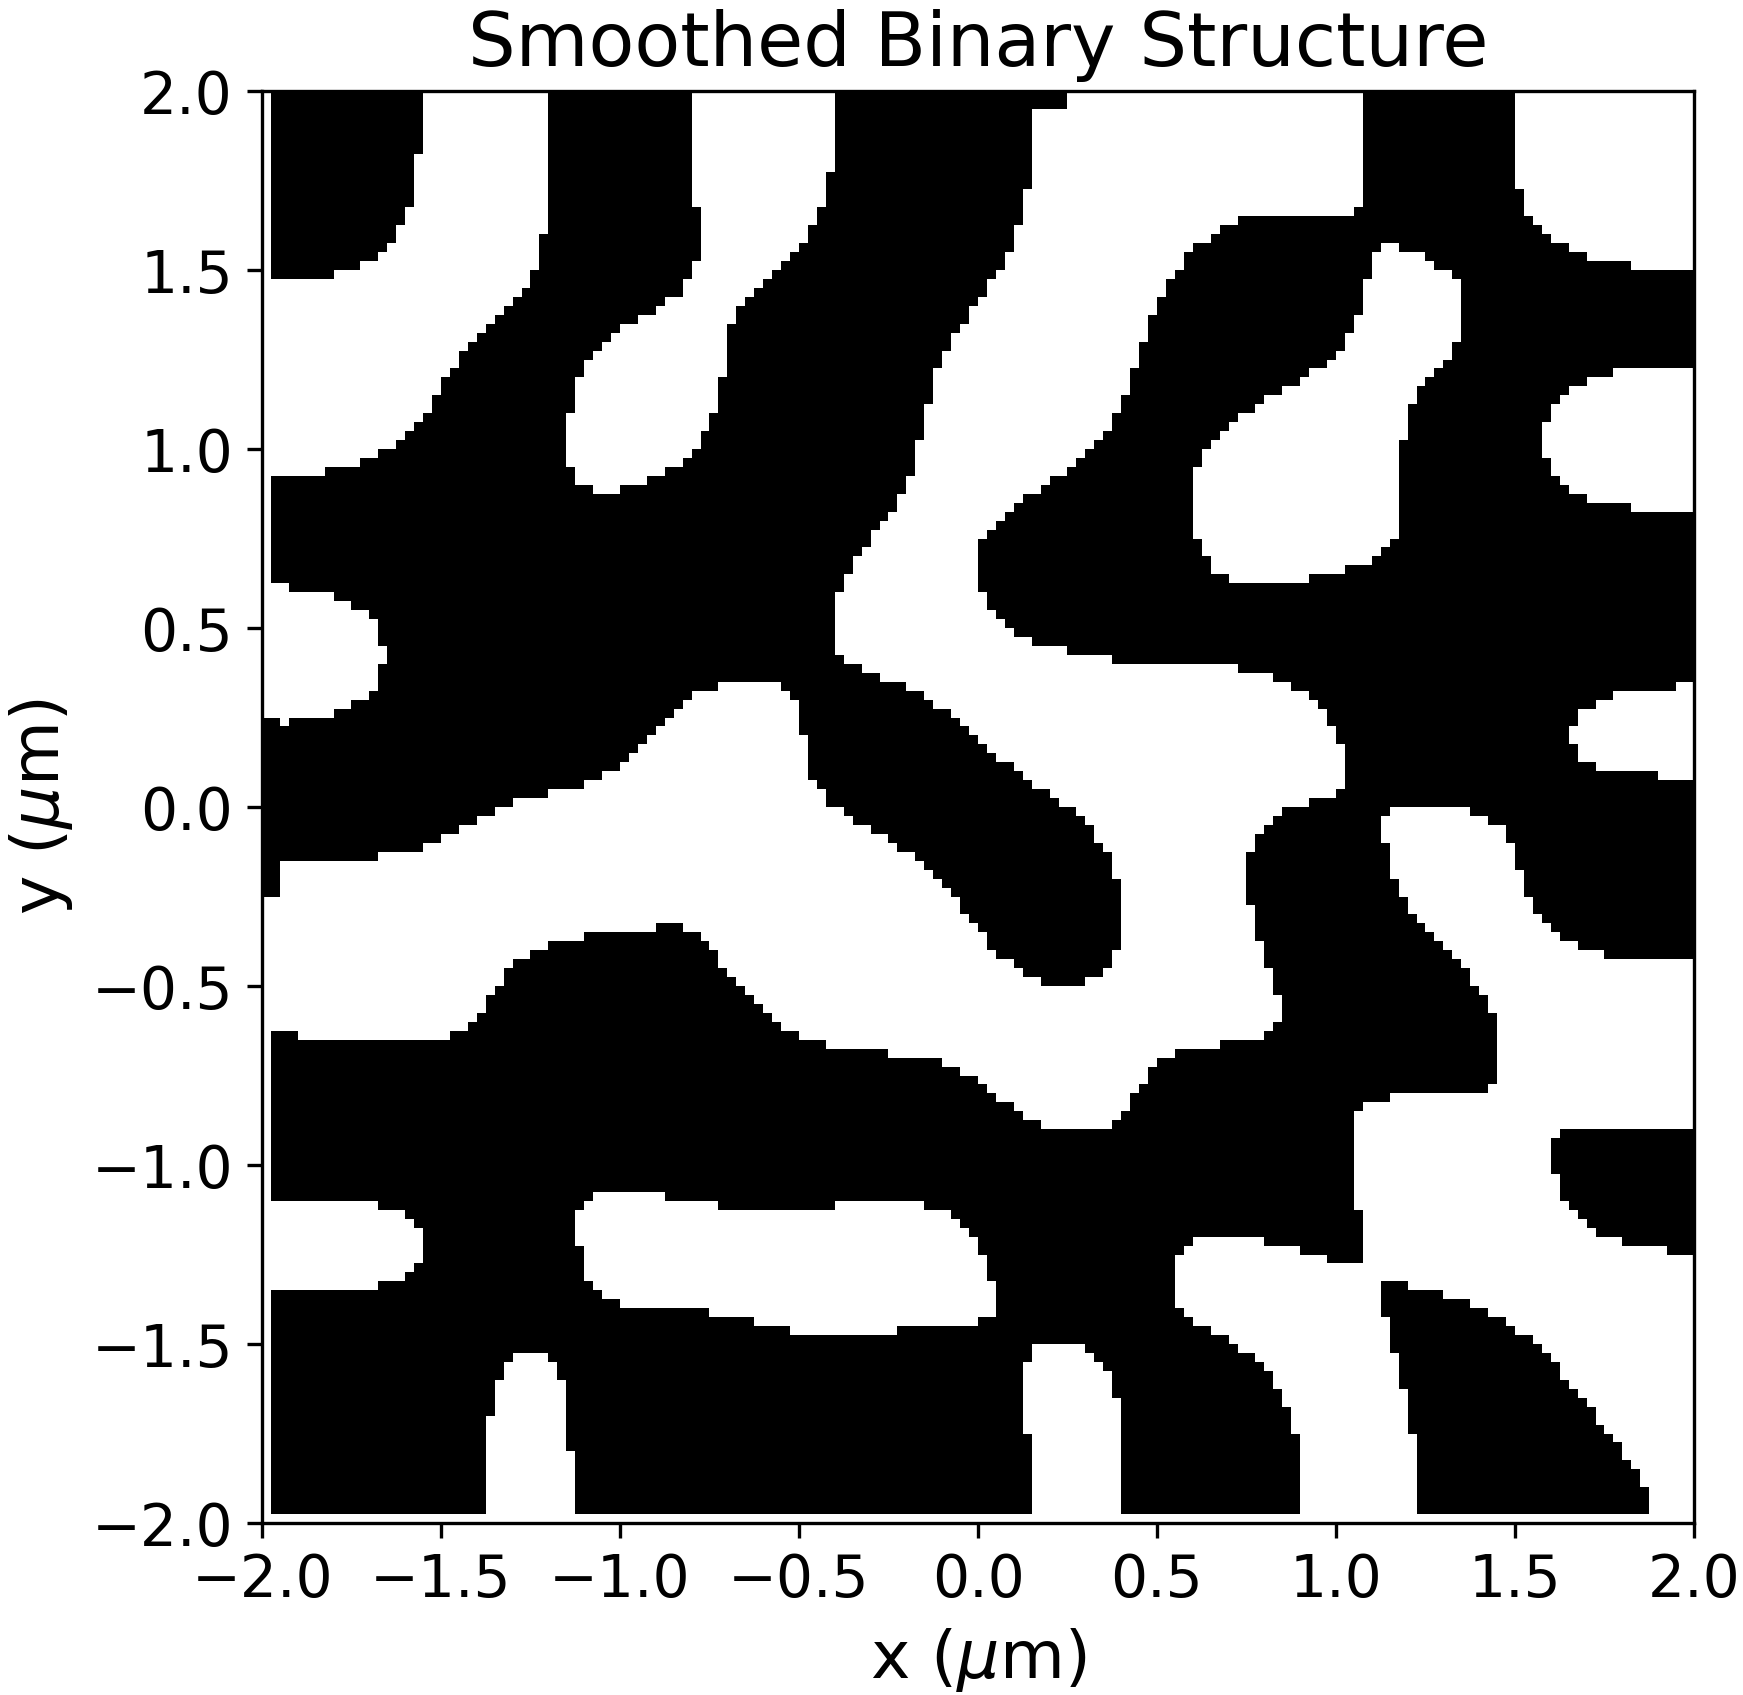
\includegraphics[width=0.7\textwidth]{img/BEND/BEND-2F-design2/Smoothed_Binary_Structure.png}
\caption{二維傅立葉積分策略應用於彎曲波導 Design 2之幾何結構圖。}
\label{fig:BEND_2F_structure_design2}
\end{figure}

\subsubsection{2D Fourier Integral on Bend Waveguide Design - parameter 3}
\label{ch:2F_BEND_Design3}
接著，將頻譜空間變數提升至 $12\times12$，進一步增加設計自由度，以評估較高維度之頻譜空間變數對彎曲波導最佳化結果之影響。
其餘 MEEP 模擬參數、光源設定及最佳化流程皆維持與 Design 1 (第~\ref{ch:2F_BEND_Design1}節)相同，以確保不同設計維度間具有一致之比較基準。

最終FoM略降至:
\begin{align}
FOM = 0.9350
\label{eq:BEND_2DF_design3_FOM}
\end{align}
採用 $12\times12$ 頻譜空間變數後，最終穿透率略降為93.50\%。雖然仍維持良好的傳輸效率，但相較於 Design 2 (第~\ref{ch:2F_BEND_Design2}節)略為下降，
表示持續增加設計自由度不一定能帶來進一步的效能提升。

接著，觀察最佳化過程中最佳FoM的變化，如圖~\ref{fig:BEND_2F_design3_Bestfom_vs_iteration}與圖~\ref{fig:BEND_2F_design3_Opt_Trajactory}所示，
相較於 Design 2 (第~\ref{ch:2F_BEND_Design2}節)，此次設計在50次迭代前的候選解大多仍維持於較低FoM區域，約於第55次迭代後，高FoM候選解才逐漸增加，
並帶動最佳FoM持續提升。這個現象說明當頻譜空間變數維度增加後，固定數量之訓練資料對設計空間的涵蓋程度可能會逐漸降低，
因此可能需要更多訓練資料或迭代次數，才能建立較準確的代理模型並且提升最佳化效率。
\begin{figure}[H]
\centering
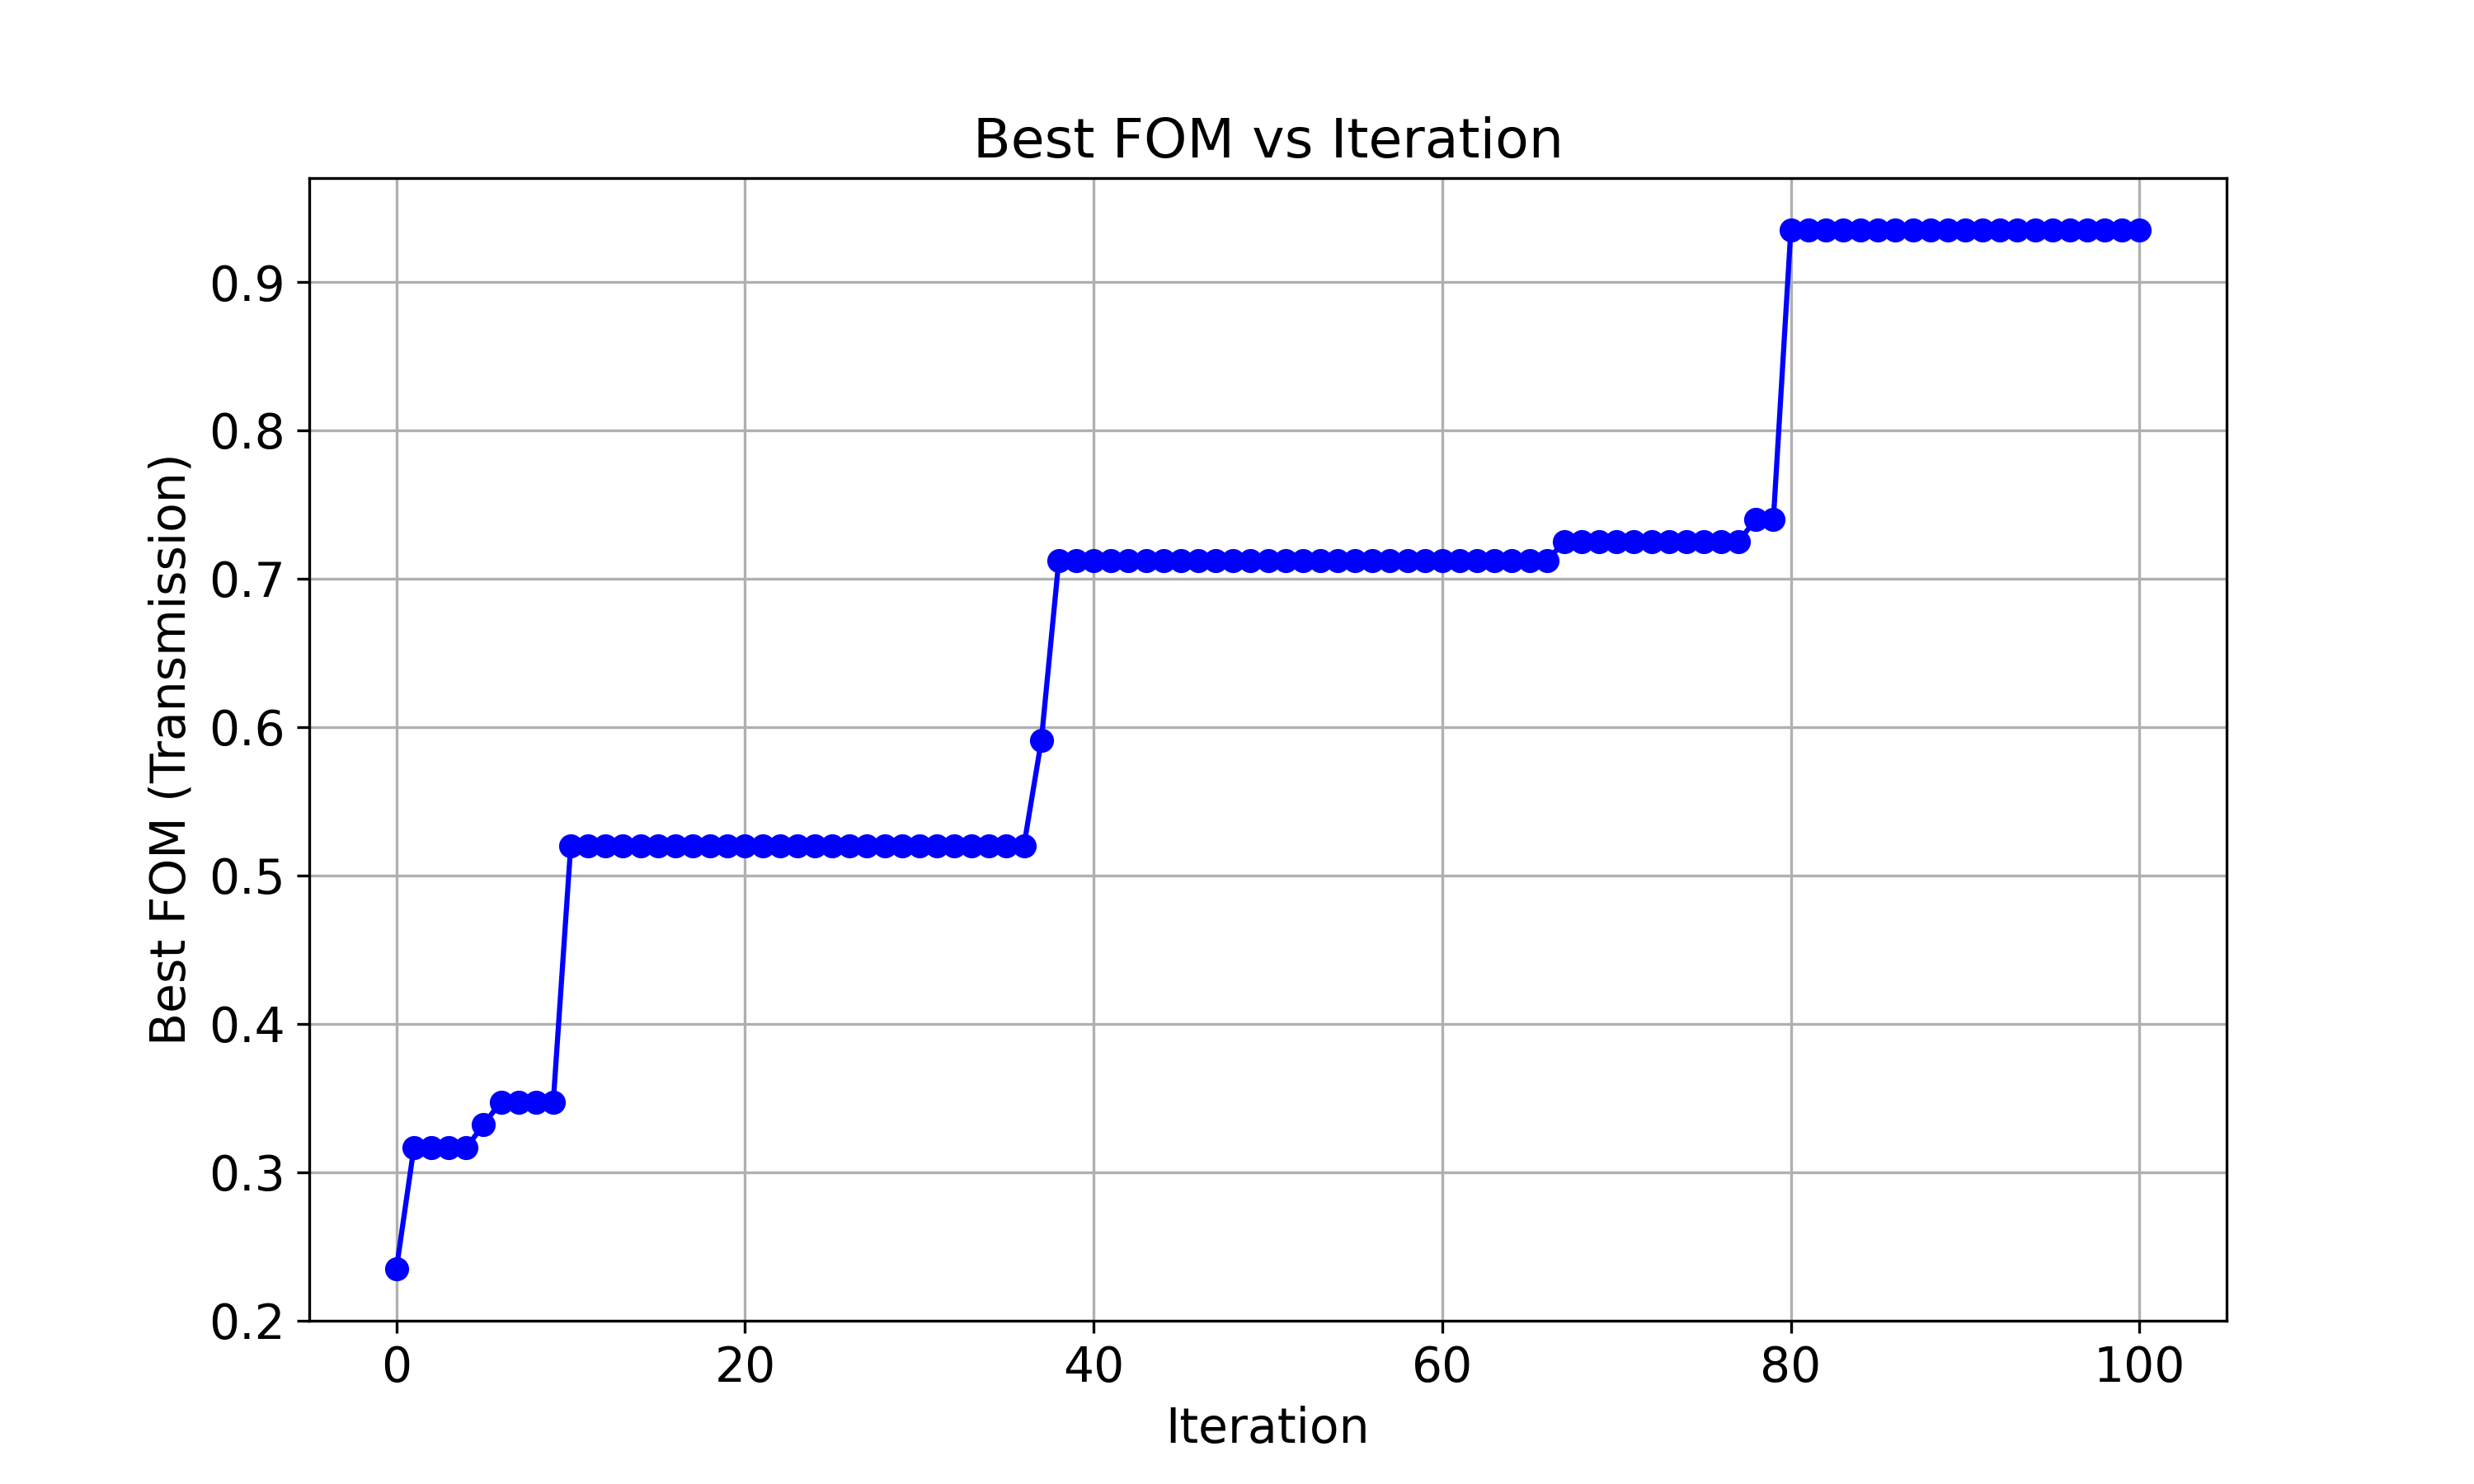
\includegraphics[width=0.9\textwidth]{img/BEND/BEND-2F-design3/fom_evolution.png}
\caption{二維傅立葉積分策略應用於彎曲波導 Design 3最佳化過程中的最佳FoM變化。}
\label{fig:BEND_2F_design3_Bestfom_vs_iteration}
\end{figure}

\begin{figure}[H]
\centering
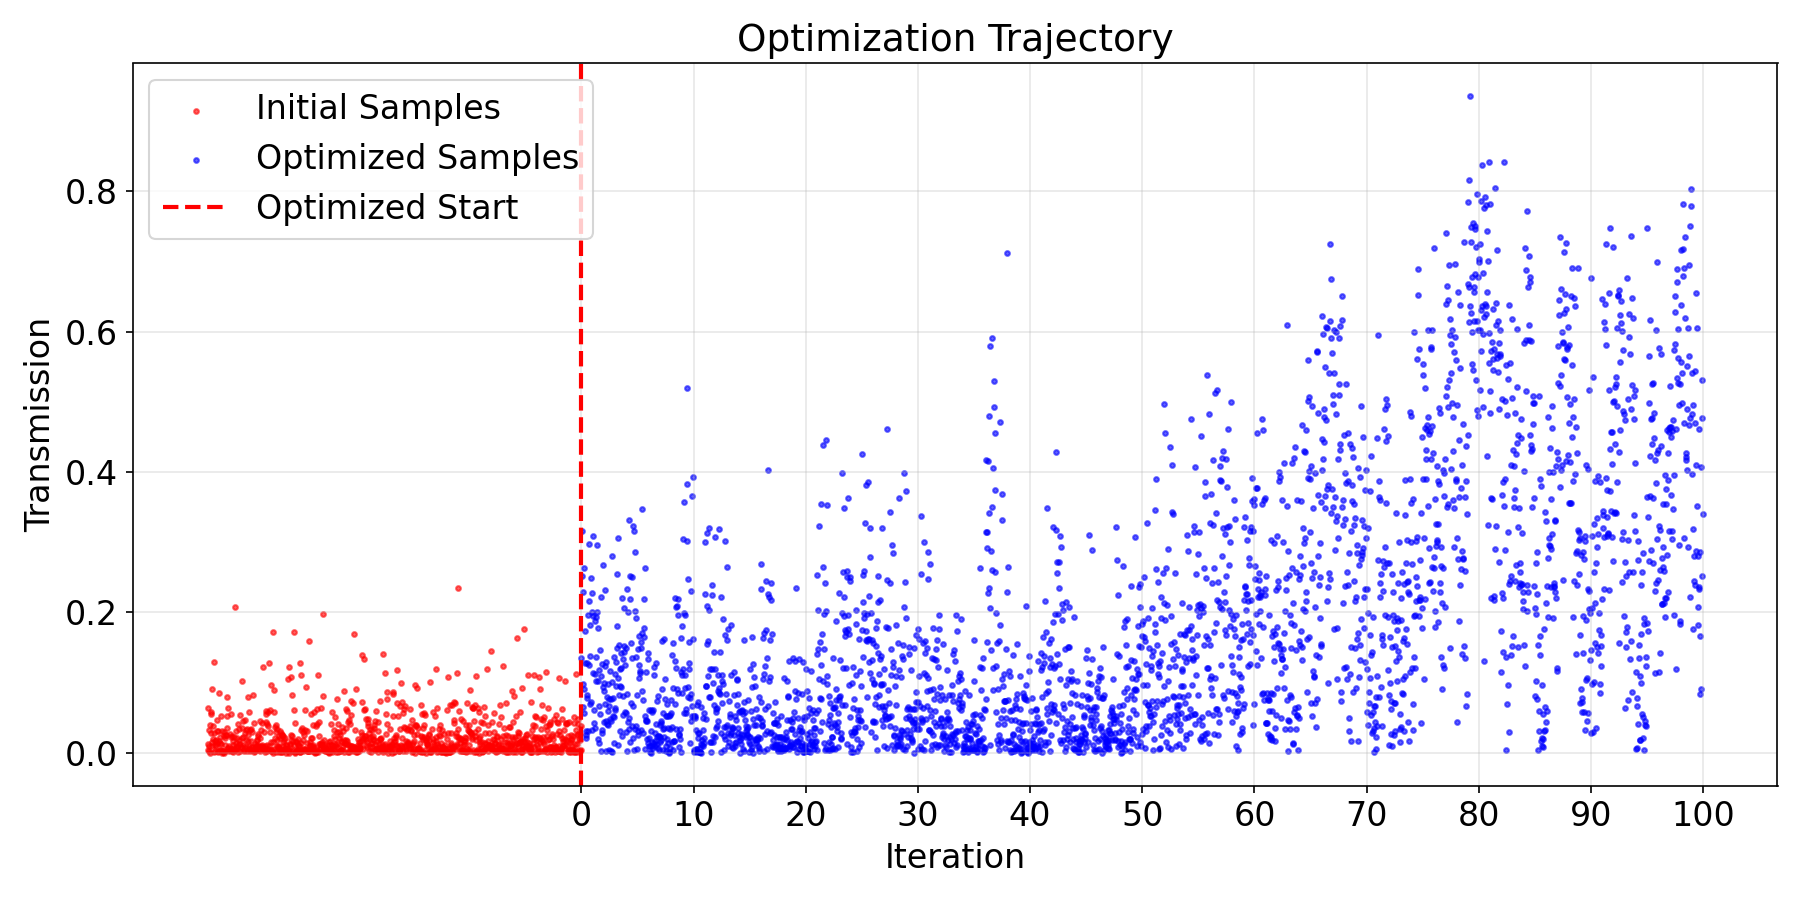
\includegraphics[width=1.0\textwidth]{img/BEND/BEND-2F-design3/transmission_trajectory.png}
\caption{二維傅立葉積分策略應用於彎曲波導 Design 3最佳化過程中的FoM變化。}
\label{fig:BEND_2F_design3_Opt_Trajactory}
\end{figure}
圖~\ref{fig:BEND_2F_DFT_design3}呈現 Design 3 之電場強度分布。由圖中可觀察到，光場仍然可以順利通過彎曲區域並耦合至輸出波導，
整體光場沒有出現明顯漏光現象，因此仍維持90\%以上之穿透率。
\begin{figure}[H]
\centering
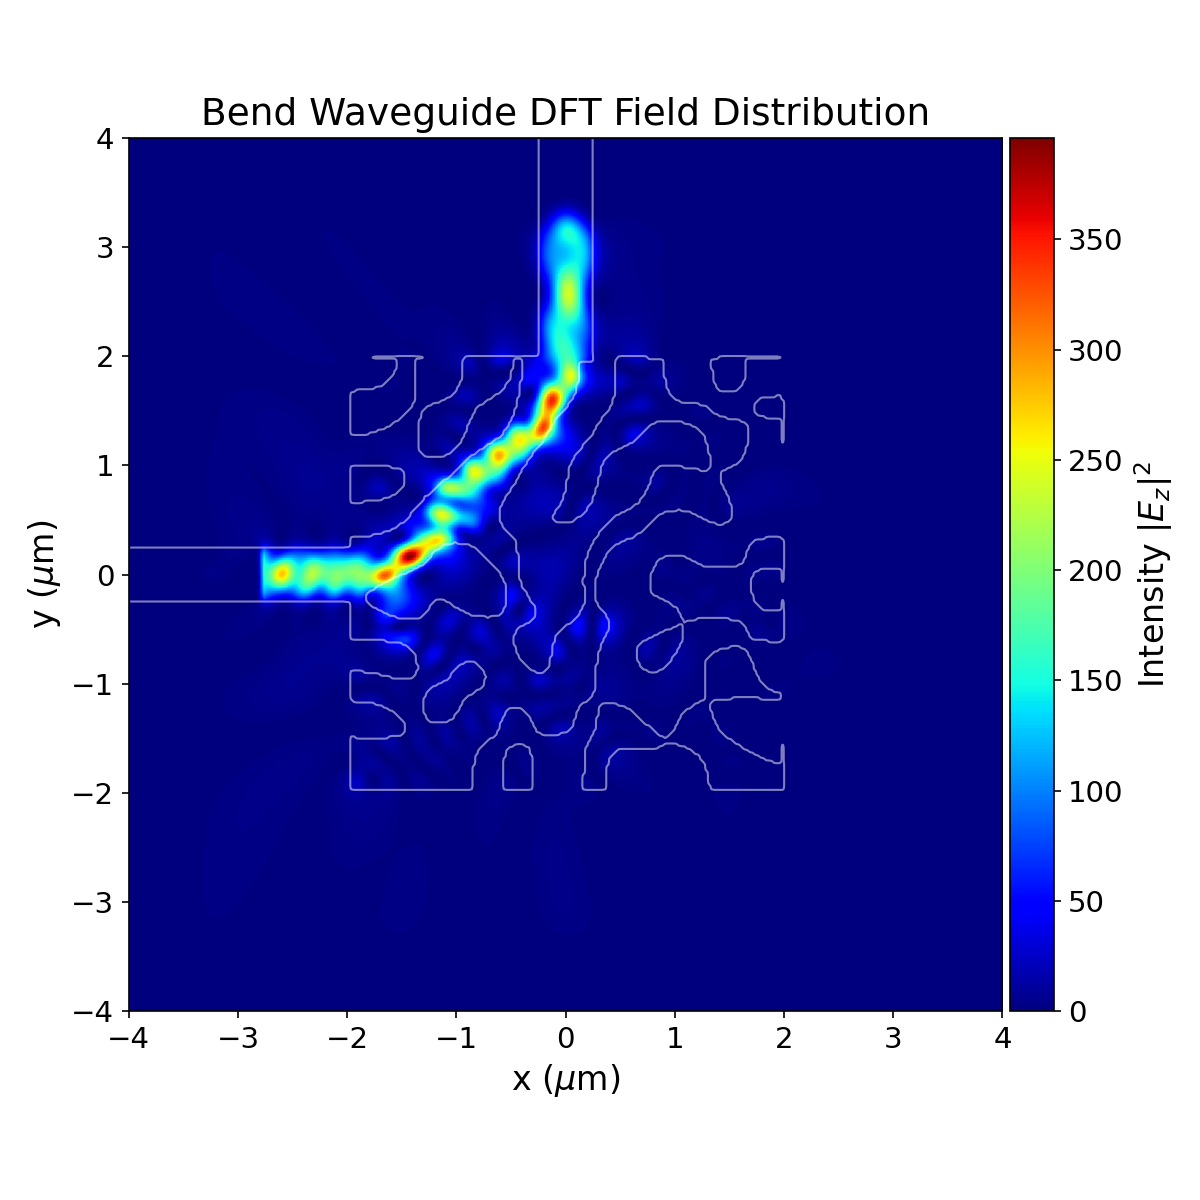
\includegraphics[width=0.8\textwidth]{img/BEND/BEND-2F-design3/final_analysis_TE0_field.png}
\caption{二維傅立葉積分策略應用於彎曲波導 Design 3之DFT電場強度分布圖。}
\label{fig:BEND_2F_DFT_design3}
\end{figure}
從圖~\ref{fig:BEND_2F_structure_design3}可以觀察到，相較於Design 2(第~\ref{ch:2F_BEND_Design2}節)，
增加頻譜空間變數的維度後，整體結構產生了更多局部幾何細節，但主要傳導光場的波導結構邊界仍然維持連續且平滑，因此仍然具有良好的光場導引能力。
\begin{figure}[H]
\centering
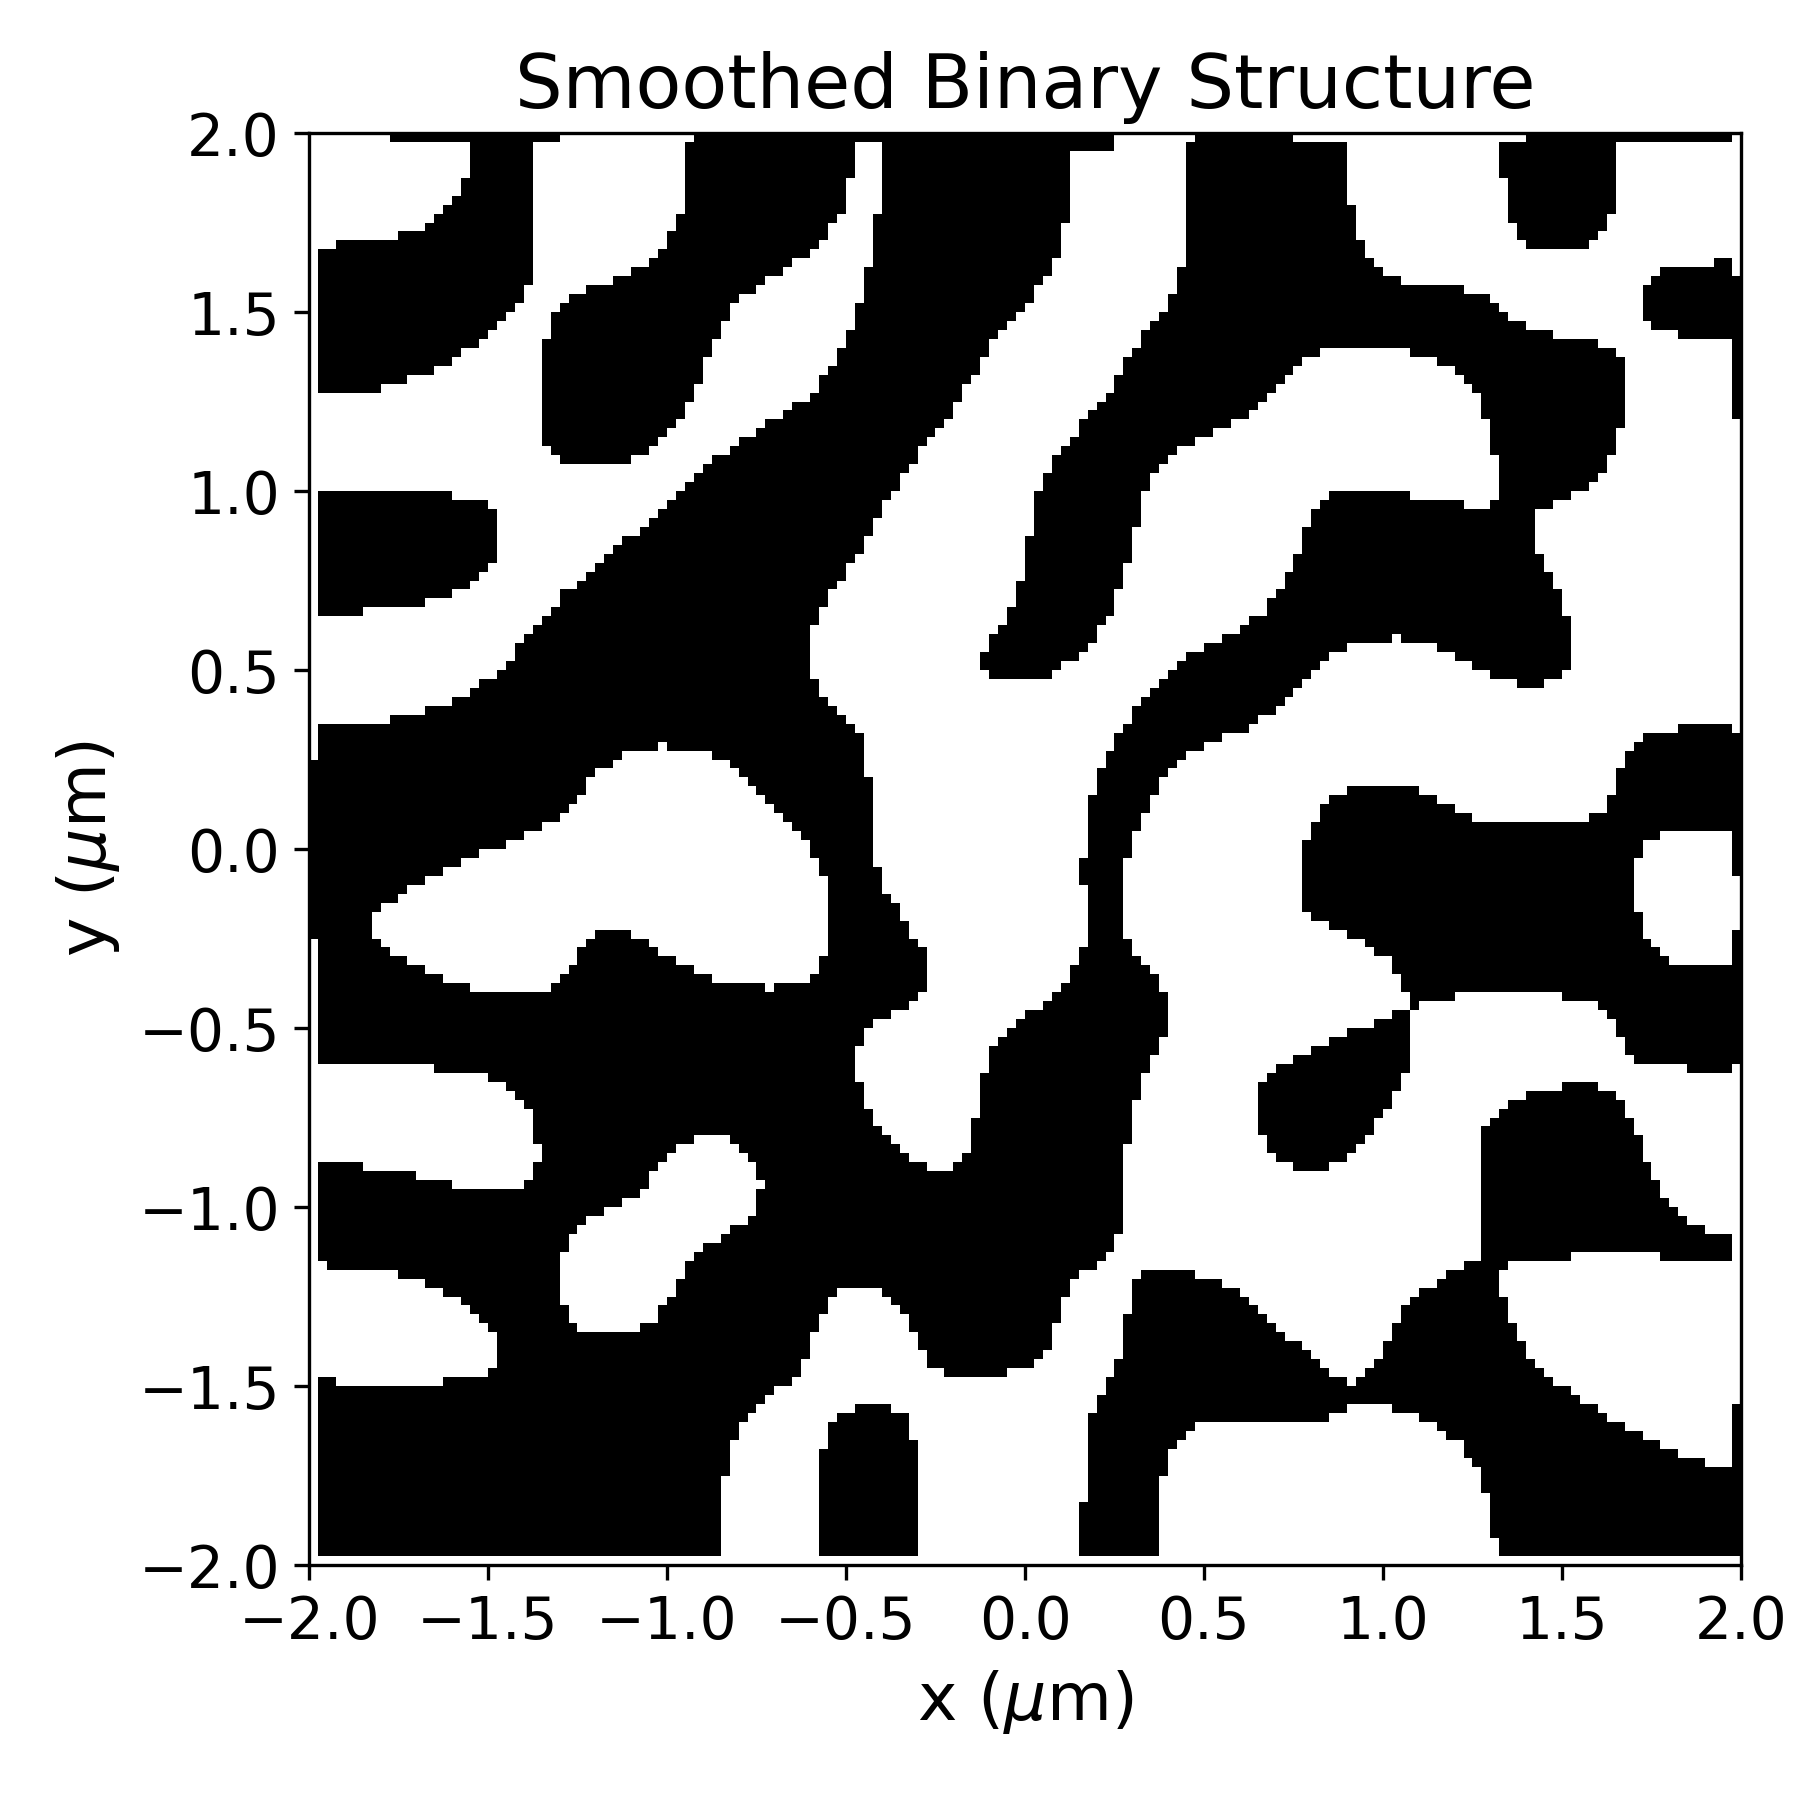
\includegraphics[width=0.7\textwidth]{img/BEND/BEND-2F-design3/Smoothed_Binary_Structure.png}
\caption{二維傅立葉積分策略應用於彎曲波導 Design 3之幾何結構圖。}
\label{fig:BEND_2F_structure_design3}
\end{figure}

\subsubsection{2D Fourier Integral on Bend Waveguide Design - parameter 4}
\label{ch:2F_BEND_Design4}
為進一步探討高維度頻譜空間變數對最佳化結果之影響，本實驗將頻譜空間變數提升至 $16\times16$。
除設計維度外，其餘 MEEP 模擬參數、光源設定及最佳化流程皆與 Design 1 (第~\ref{ch:2F_BEND_Design1}節)相同，以分析增加設計自由度後對彎曲波導最佳化效能之影響。

最終FoM降為:
\begin{align}
FOM = 0.4683
\label{eq:BEND_2DF_design4_FOM}
\end{align}
當頻譜空間變數增加至 $16\times16$ 時，最終穿透率大幅下降到46.83\%。
從圖~\ref{fig:BEND_2F_design4_Bestfom_vs_iteration}可以觀察到，最佳FoM仍然隨著迭代次數增加而穩定提升，但整體只呈現小幅度成長，
並沒有出現像是 Design 2 (第~\ref{ch:2F_BEND_Design2}節)那樣明顯的突破。
\begin{figure}[H]
\centering
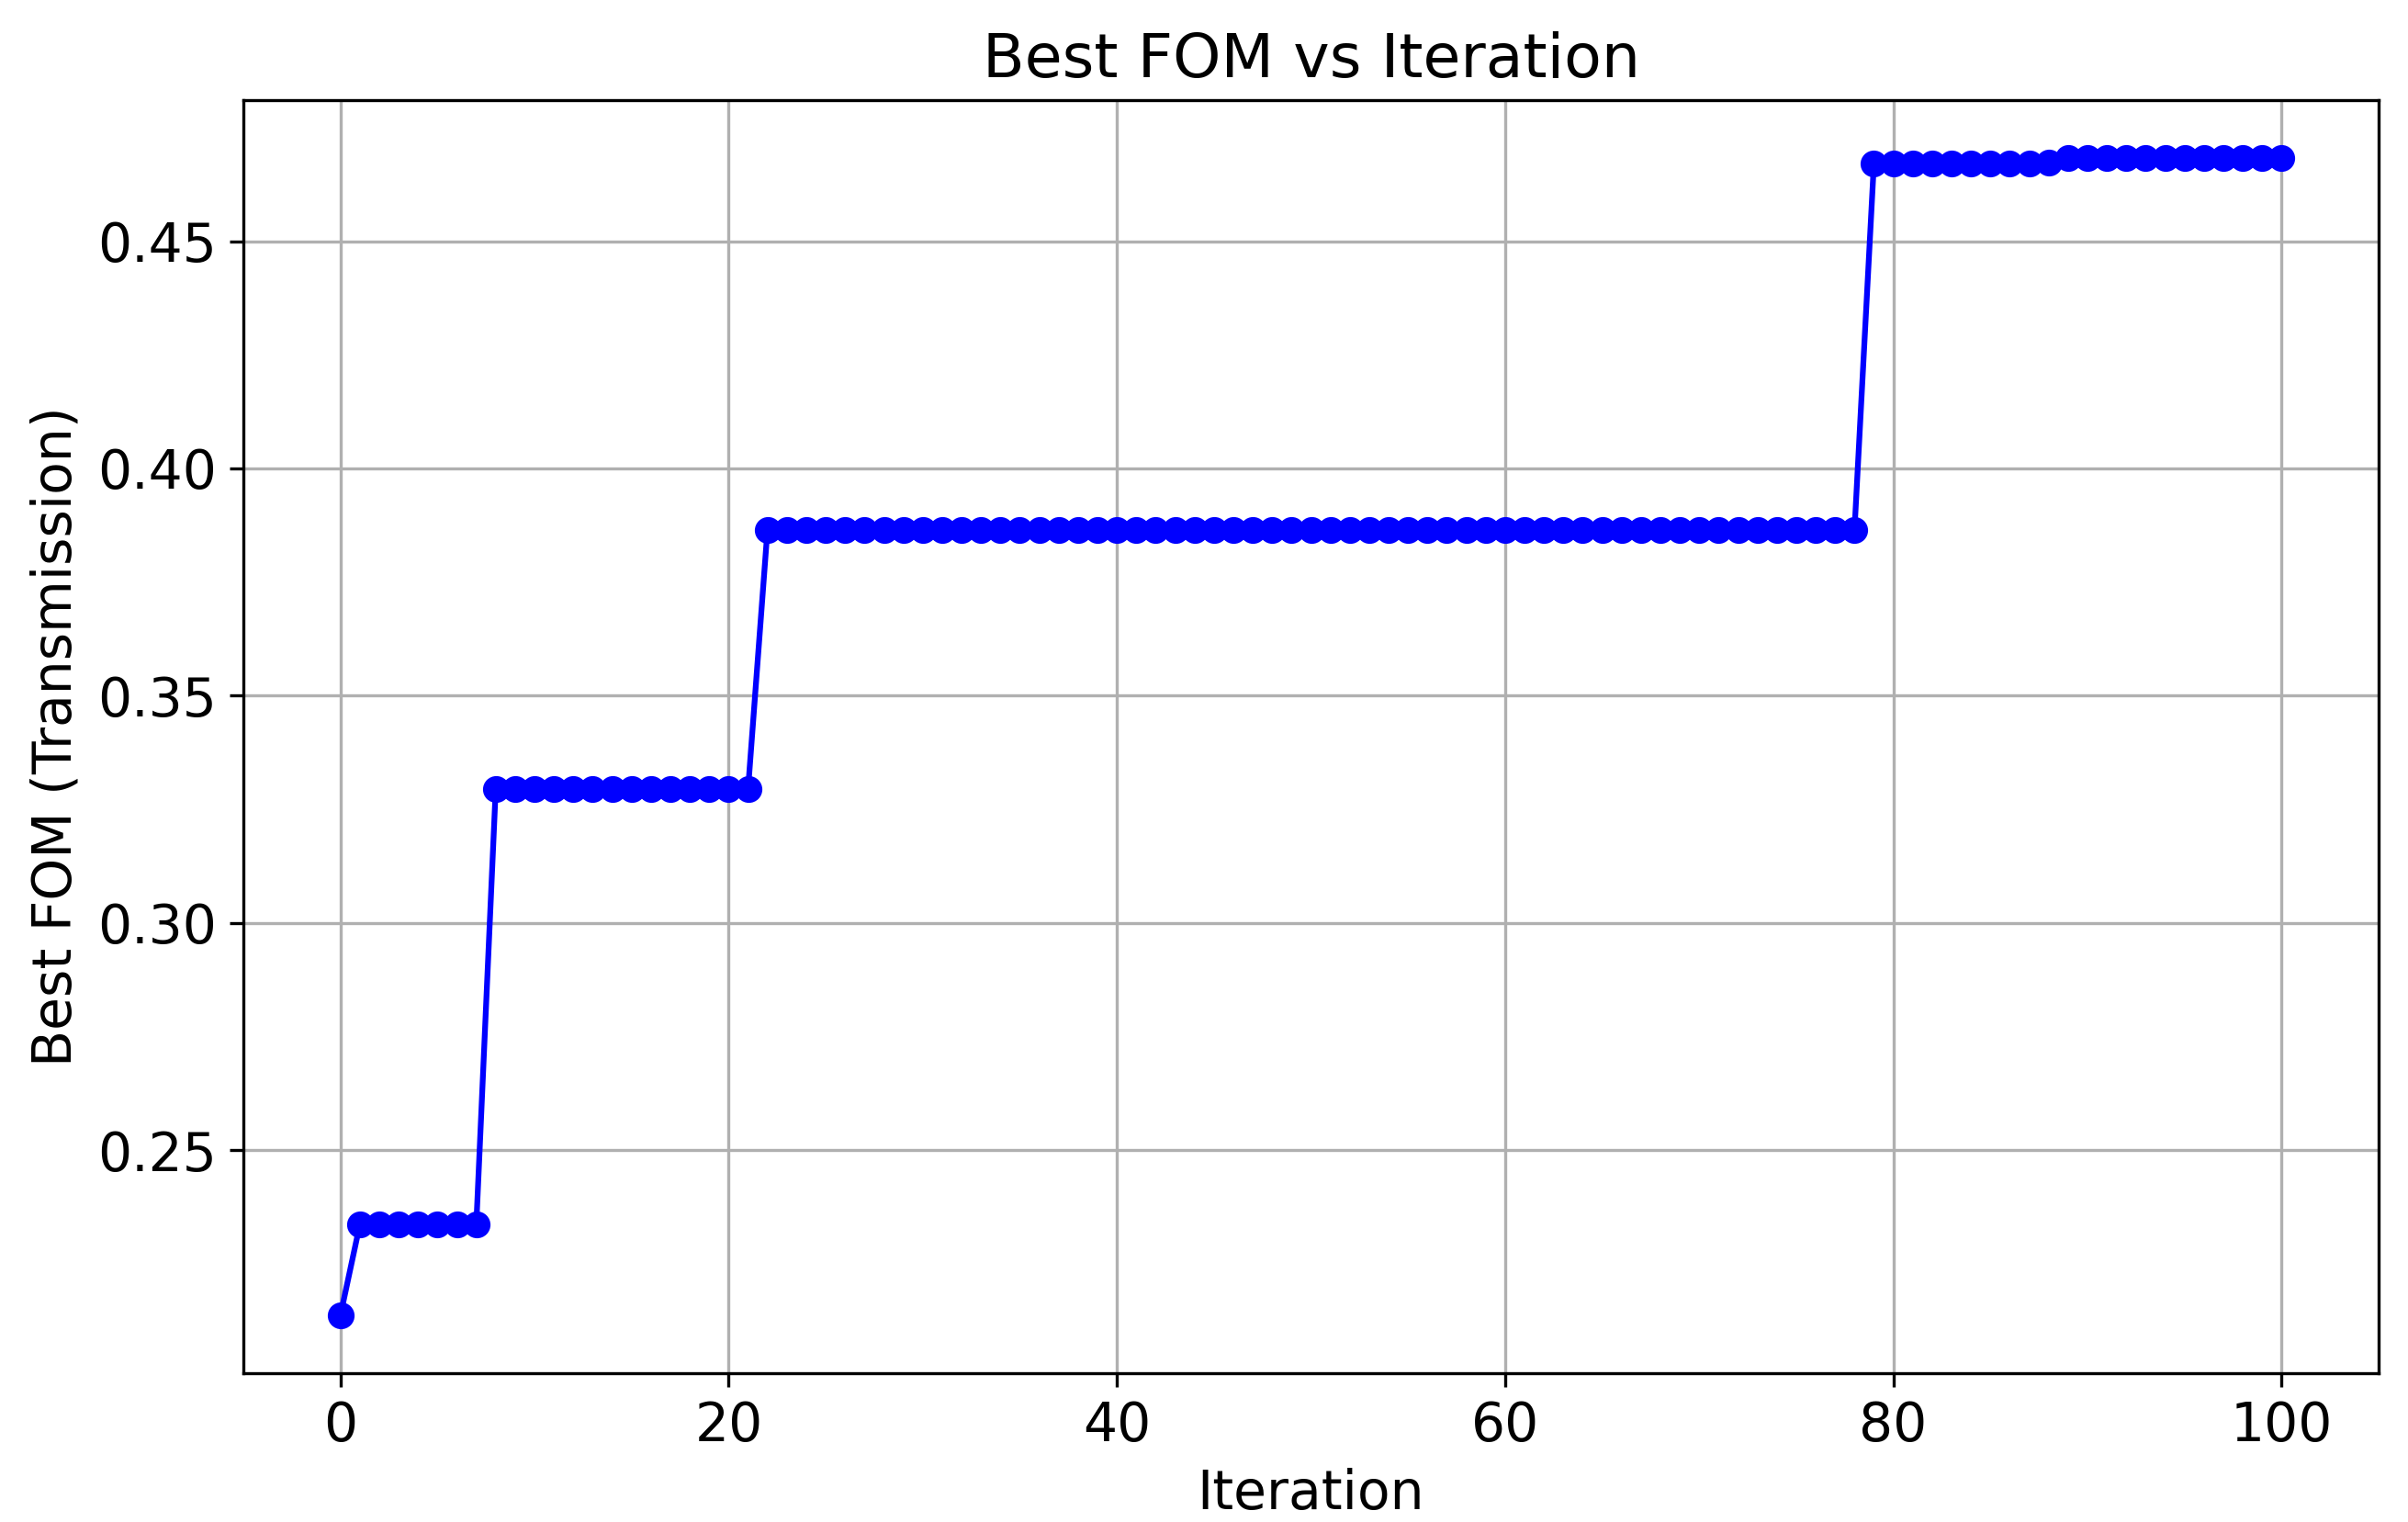
\includegraphics[width=0.9\textwidth]{img/BEND/BEND-2F-design4/fom_evolution.png}
\caption{二維傅立葉積分策略應用於彎曲波導 Design 4最佳化過程中的最佳FoM變化。}
\label{fig:BEND_2F_design4_Bestfom_vs_iteration}
\end{figure}
此外，從圖~\ref{fig:BEND_2F_design4_Opt_Trajactory}可以觀察到，大約在第40至85次的迭代中，大部分候選解都集中於低FoM區域，
高FoM候選解相對稀少，由於此研究項目的各設計參數皆使用相同的初始資料量(1000筆)與相同之迭代次數(100次)，
當頻譜空間變數增加後，每一筆資料對設計空間之涵蓋能力相對降低，因此可能需要更多訓練資料或更長的迭代次數，才能夠更充分地搜尋高維度設計空間並獲得較佳的結果。
\begin{figure}[H]
\centering
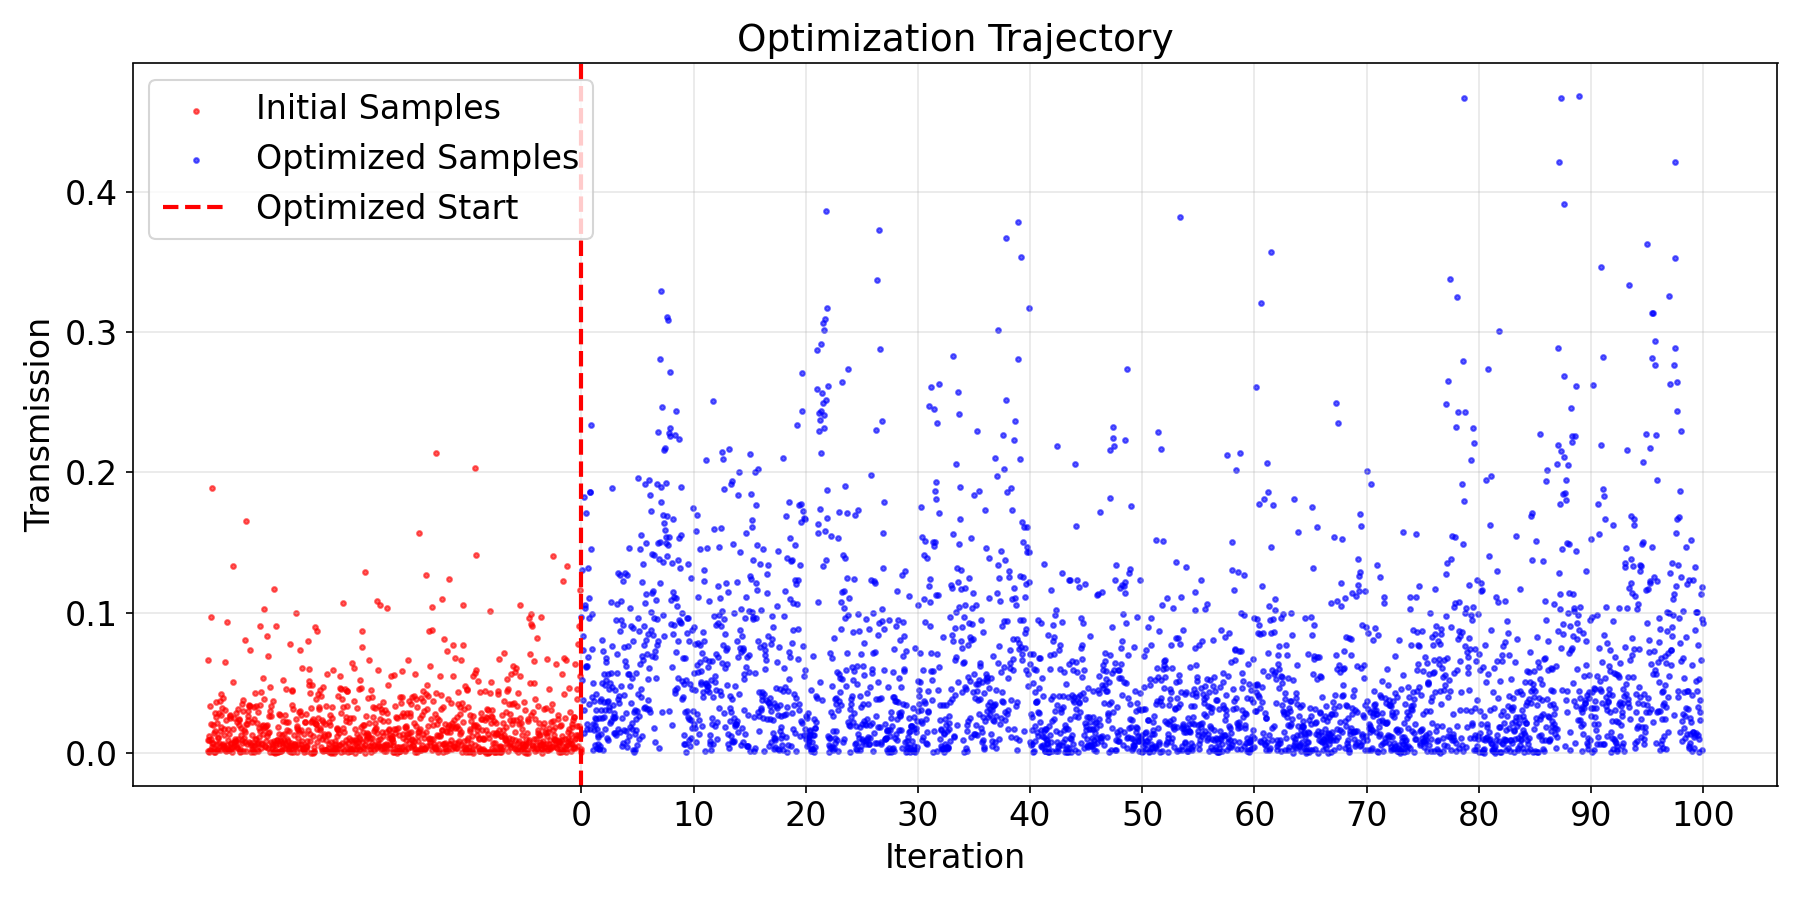
\includegraphics[width=1.0\textwidth]{img/BEND/BEND-2F-design4/transmission_trajectory.png}
\caption{二維傅立葉積分策略應用於彎曲波導 Design 4最佳化過程中的FoM變化。}
\label{fig:BEND_2F_design4_Opt_Trajactory}
\end{figure}

由圖~\ref{fig:BEND_2F_DFT_design4}可觀察到，
相較於 Design 3(第~\ref{ch:2F_BEND_Design3}節)，增加至 $16\times16$ 頻譜空間變數後，最佳化結構呈現更多細小且破碎的局部幾何特徵，
使彎曲區域的結構連續性大幅降低。從電場分布(圖~\ref{fig:BEND_2F_structure_design4})也可以觀察到光場因為破碎的幾何結構而產生較明顯的能量洩漏，
導致進入輸出波導之光場強度下降，最終使穿透率大幅降至46.83\%。
\begin{figure}[H]
\centering
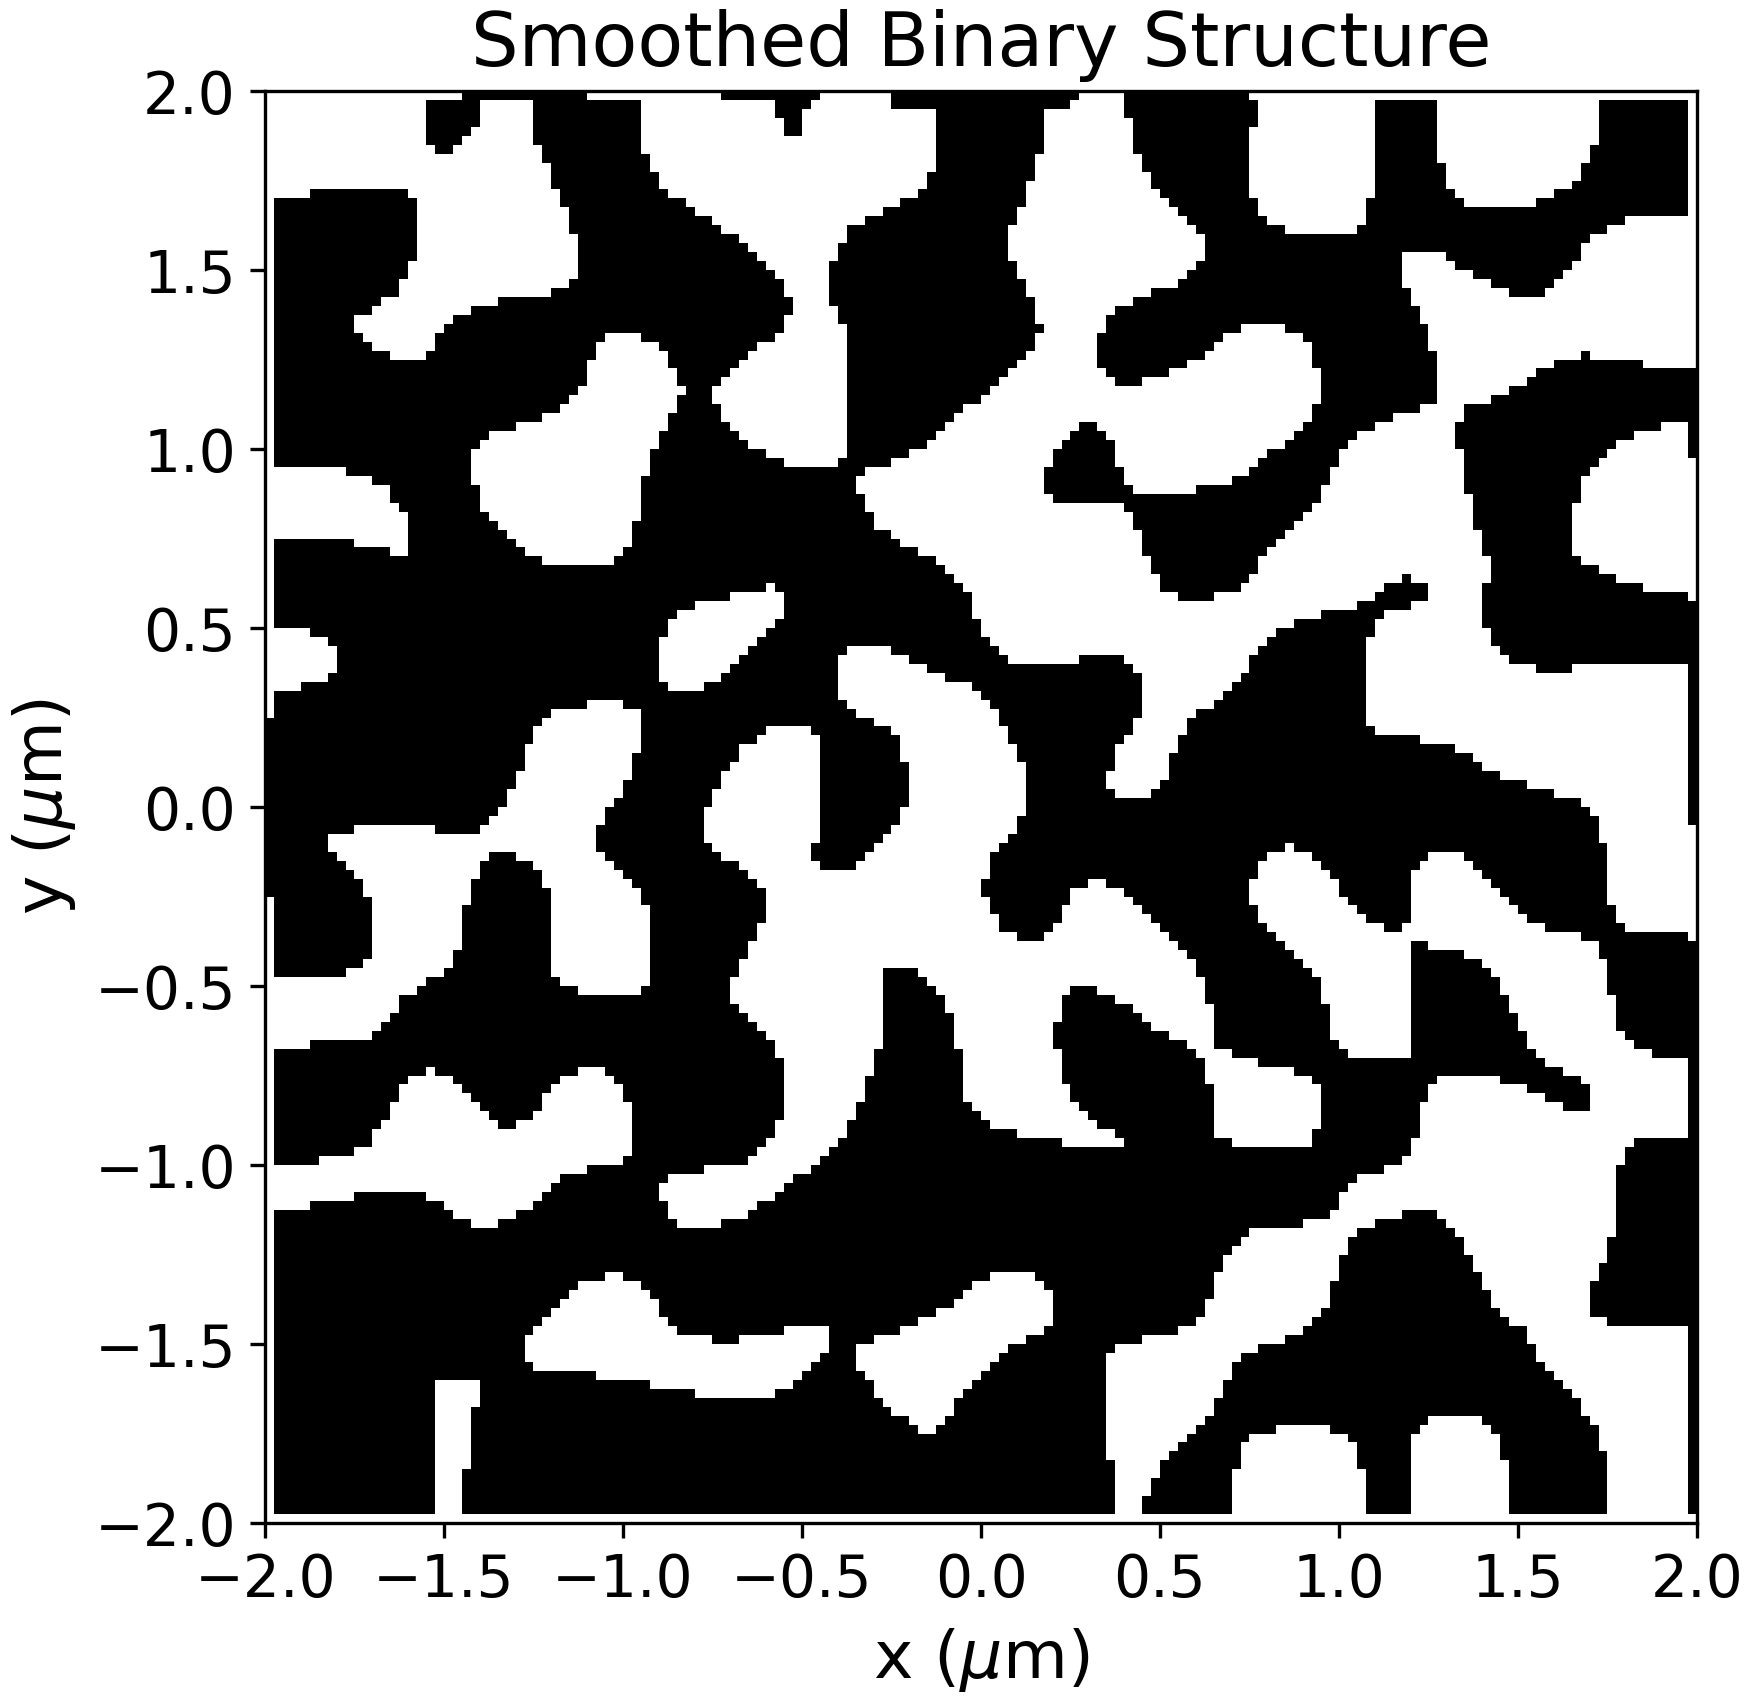
\includegraphics[width=0.7\textwidth]{img/BEND/BEND-2F-design4/Smoothed_Binary_Structure.png}
\caption{二維傅立葉積分策略應用於彎曲波導 Design 4之幾何結構圖。}
\label{fig:BEND_2F_structure_design4}
\end{figure}

\begin{figure}[H]
\centering
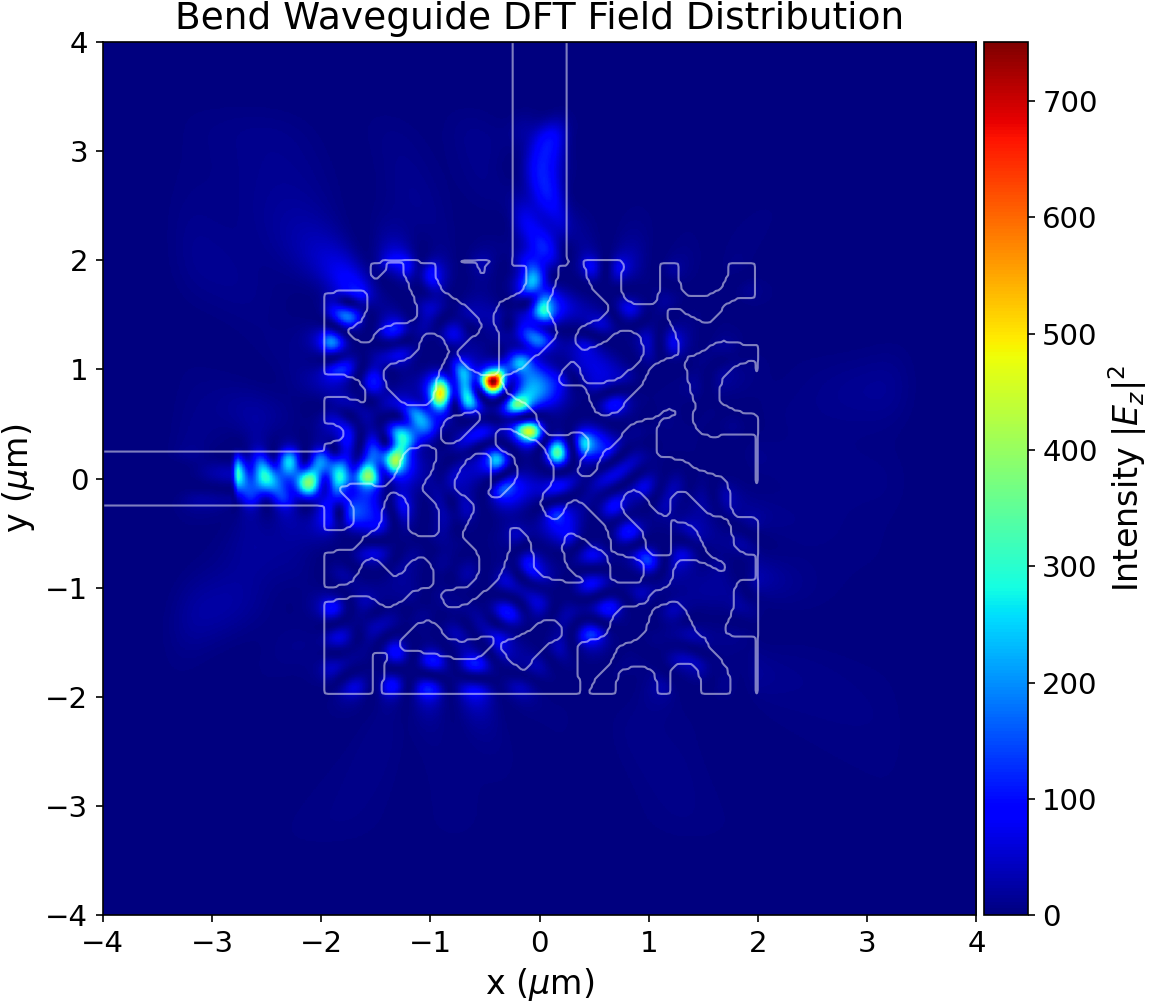
\includegraphics[width=0.8\textwidth]{img/BEND/BEND-2F-design4/final_analysis_TE0_field.png}
\caption{二維傅立葉積分策略應用於彎曲波導 Design 4之DFT電場強度分布圖。}
\label{fig:BEND_2F_DFT_design4}
\end{figure}

\subsubsection{2D Fourier Integral on Bend Waveguide Design - parameter 5}
\label{ch:2F_BEND_Design5}
最後，將頻譜空間變數進一步提升至 $20\times20$，以評估更高設計自由度下二維傅立葉積分方法之最佳化能力。
其餘 MEEP 模擬參數、光源設定及最佳化流程皆維持與前述實驗一致，以探討高維度頻譜空間變數對最佳化結果之影響

最終FoM降為:
\begin{align}
FOM = 0.3167
\label{eq:BEND_2DF_design5_FOM}
\end{align}
當頻譜空間變數提升至 $20\times20$ 時，最終穿透率進一步下降為31.67\%。
從圖~\ref{fig:BEND_2F_design5_Bestfom_vs_iteration}可以觀察到，最佳FoM於第2次迭代後趨於平坦，後續迭代無法有效找到更好的候選結構。
從圖~\ref{fig:BEND_2F_design5_Opt_Trajactory}中也可以發現，大部分候選解的FoM都是集中在接近零的低分區域，高FoM候選解極為稀少，
這表示在此高維度設計空間下，固定資料量與迭代次數已經不足以有效探索可能的高效能結構。
\begin{figure}[H]
\centering
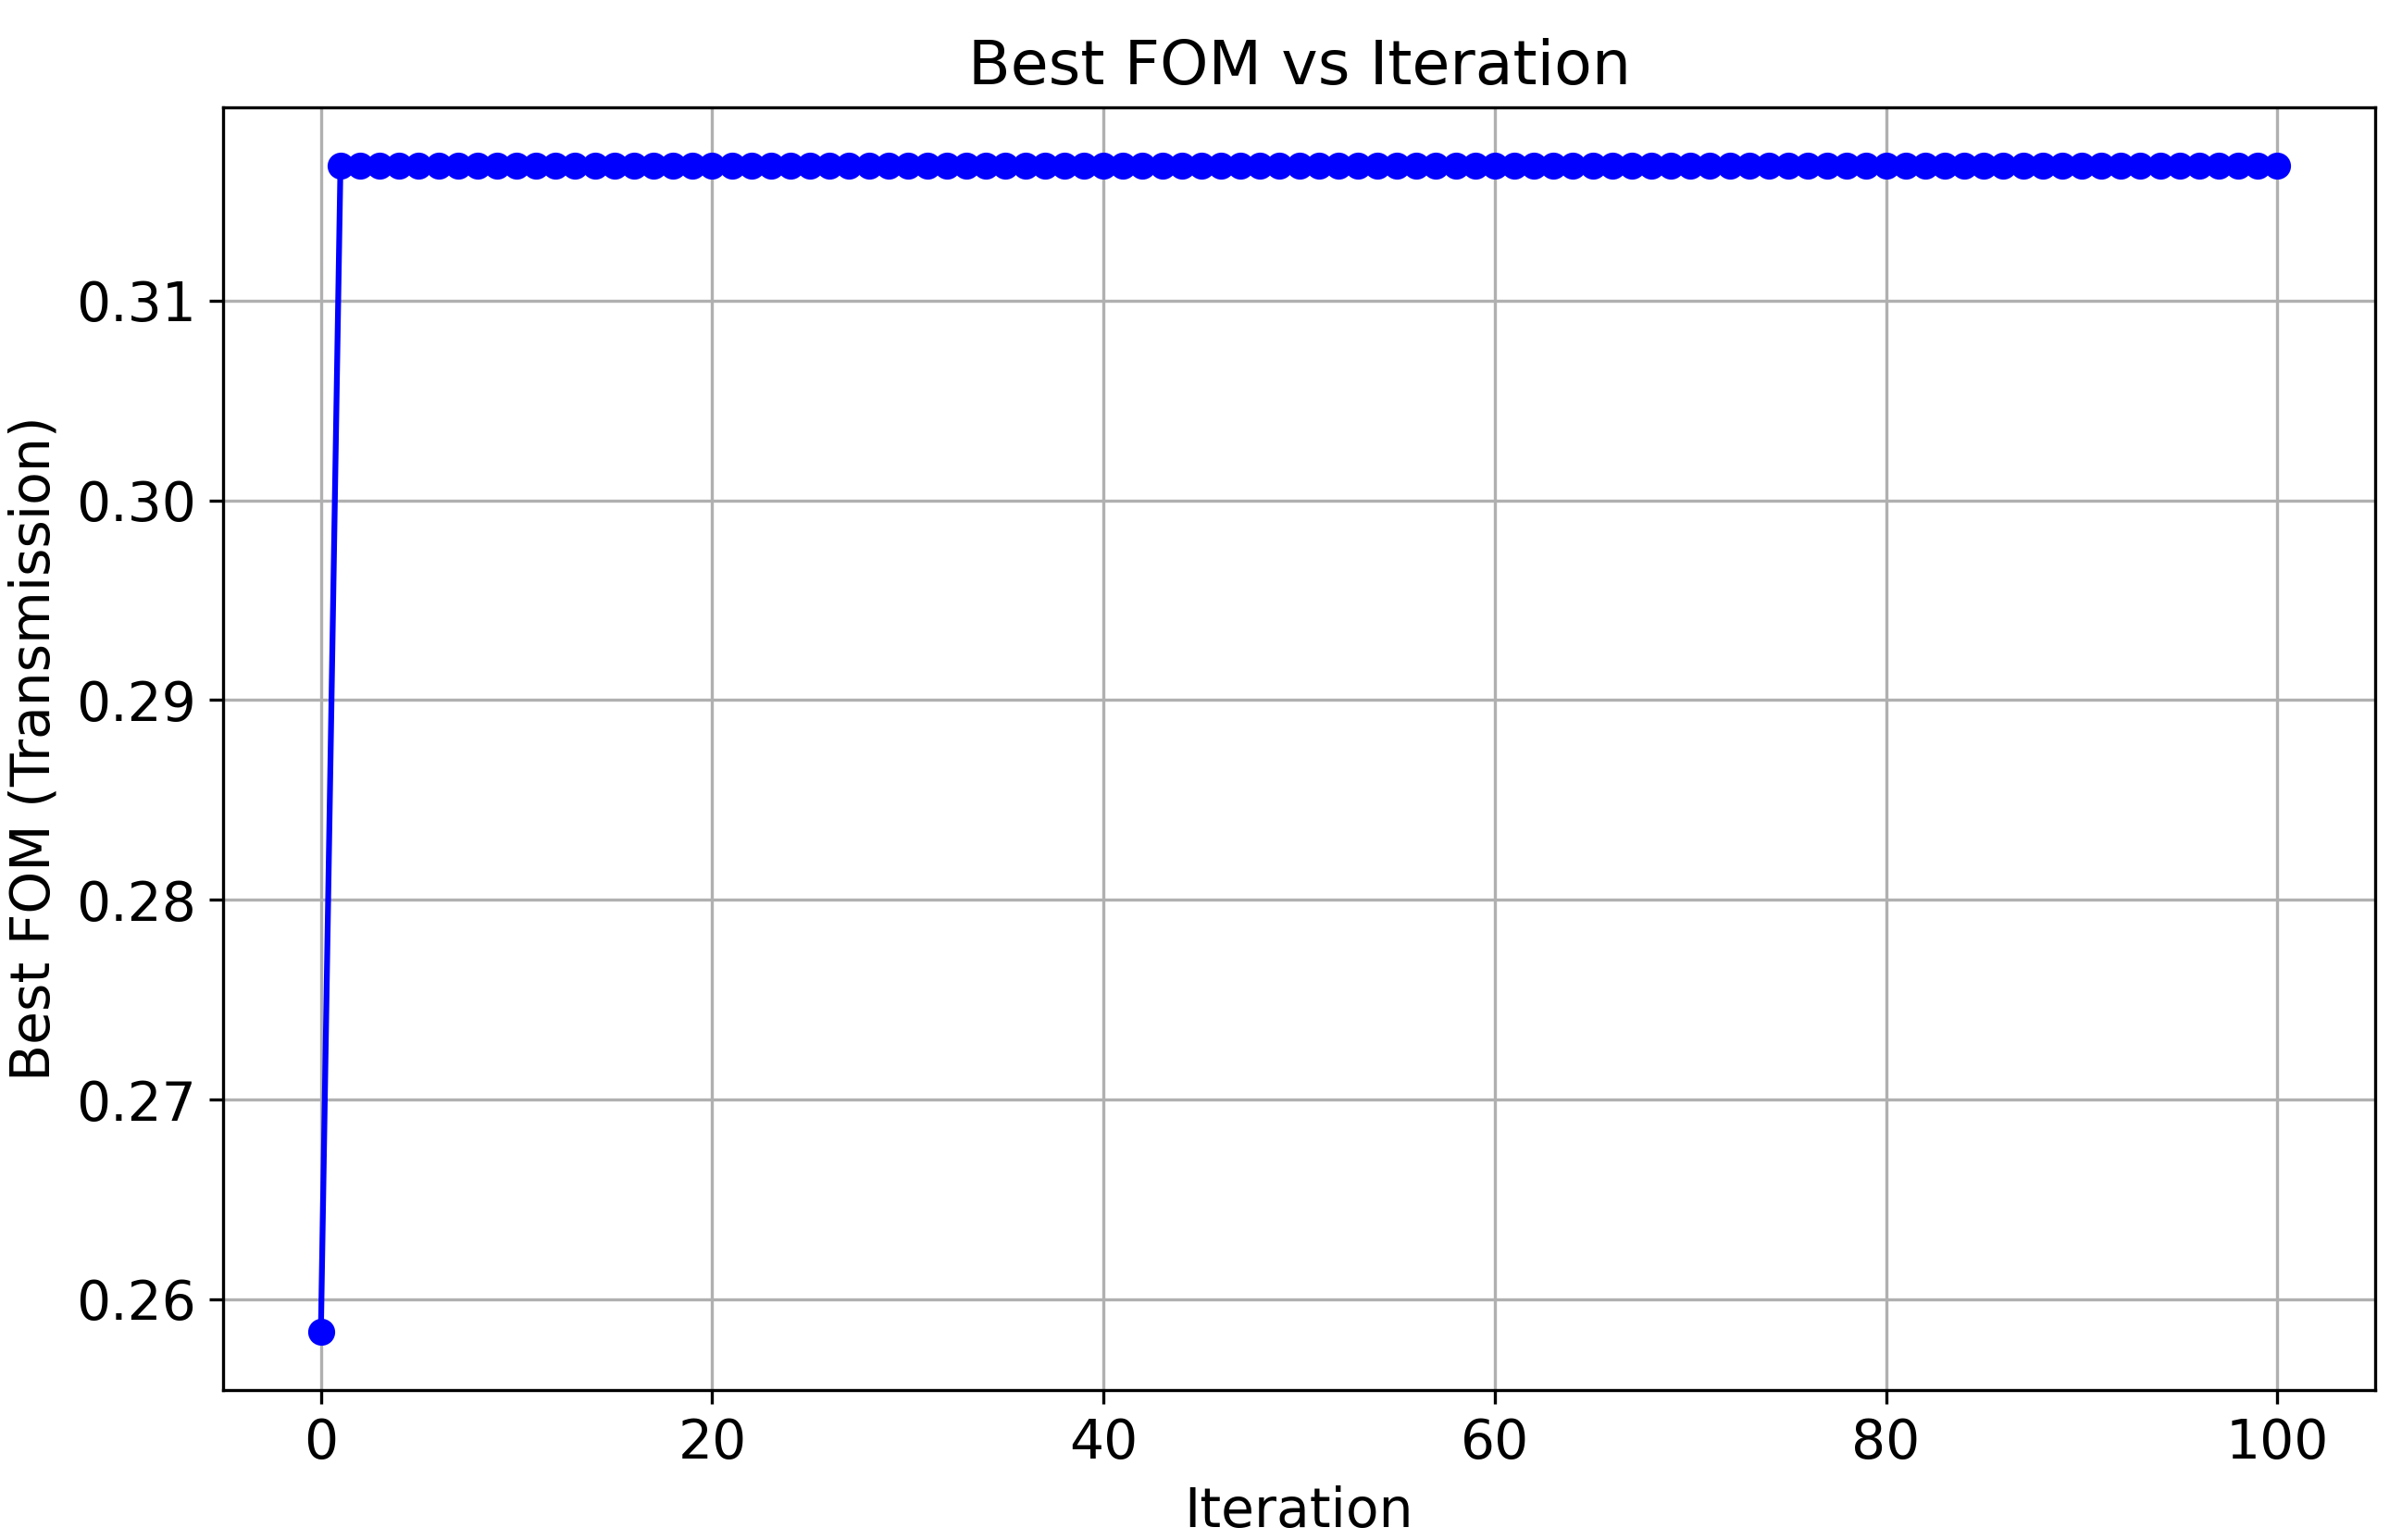
\includegraphics[width=0.9\textwidth]{img/BEND/BEND-2F-design5/fom_evolution.png}
\caption{二維傅立葉積分策略應用於彎曲波導 Design 5最佳化過程中的最佳FoM變化。}
\label{fig:BEND_2F_design5_Bestfom_vs_iteration}
\end{figure}

\begin{figure}[H]
\centering
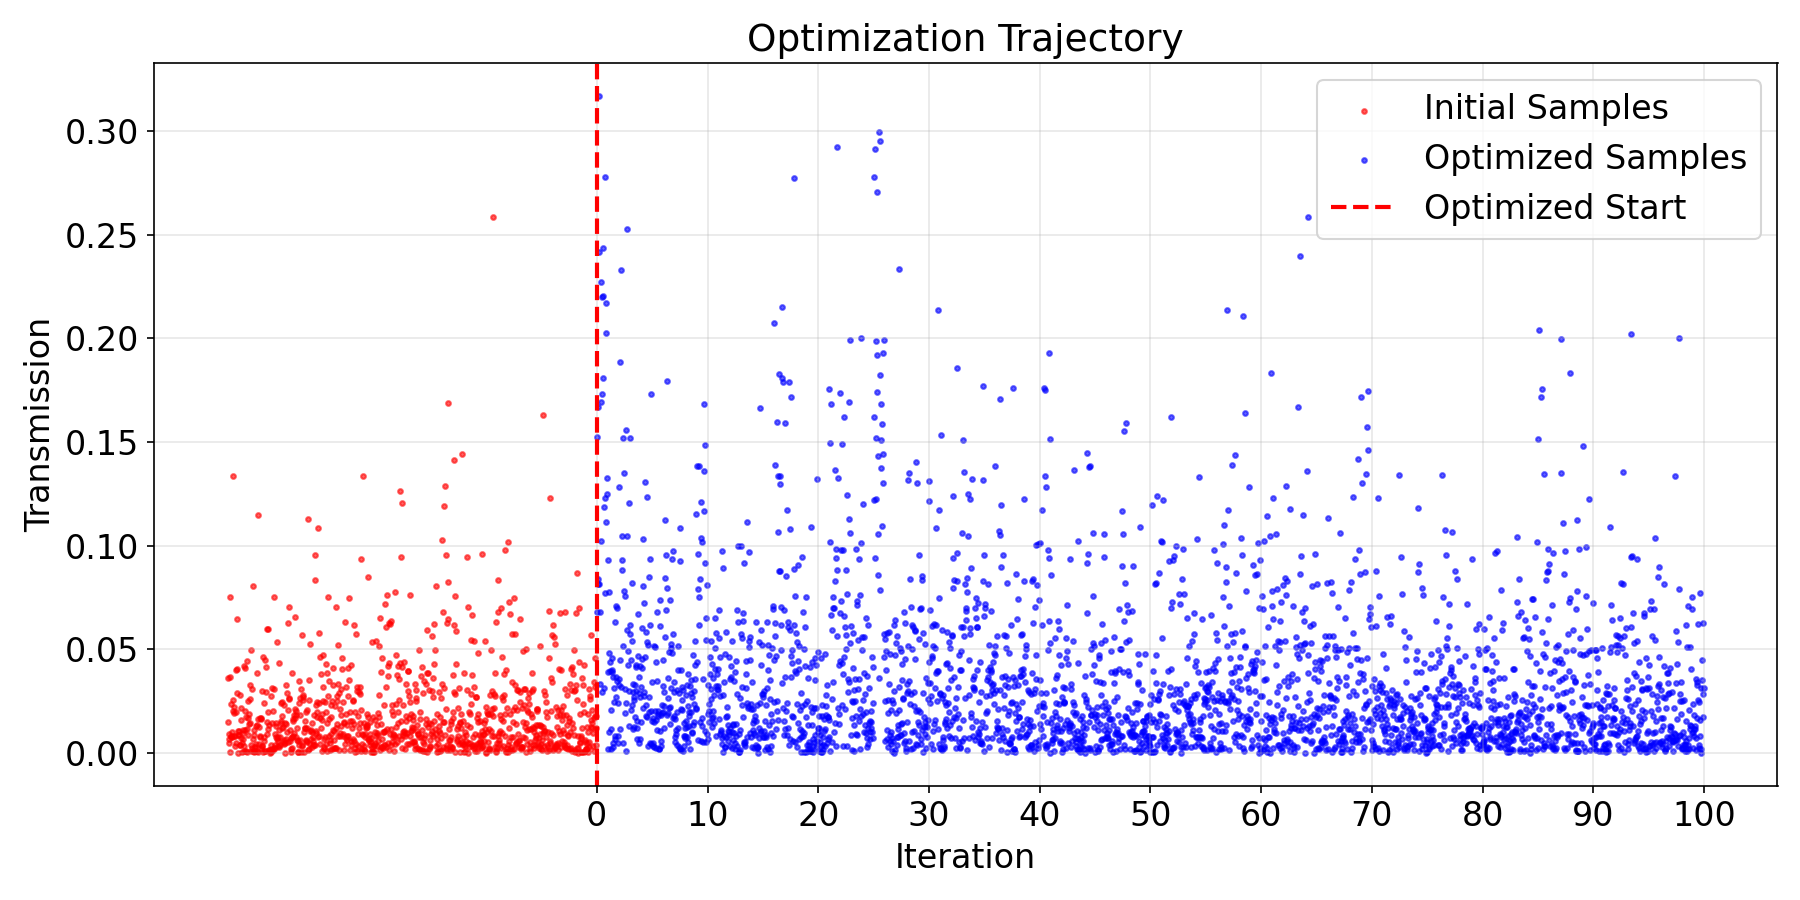
\includegraphics[width=1.0\textwidth]{img/BEND/BEND-2F-design5/transmission_trajectory.png}
\caption{二維傅立葉積分策略應用於彎曲波導 Design 5最佳化過程中的FoM變化。}
\label{fig:BEND_2F_design5_Opt_Trajactory}
\end{figure}

從圖~\ref{fig:BEND_2F_DFT_design5}與圖~\ref{fig:BEND_2F_structure_design5}中可以觀察到，當頻譜空間變數提升至 $20\times20$ 時，
最佳化結構雖然產生了更多細節，但整體幾何結構變得更加破碎且缺乏連續性，導致電場完全無法有效在結構中傳播，
最終穿透率大幅下降至31.67\%。

此結果也說明，增加設計空間維度並未能有效改善結構效能，反而提高搜尋空間複雜度，使演算法在固定資料量下更難找到具有良好傳輸效率的結構，最終造成穿透率下降。

\begin{figure}[H]
\centering
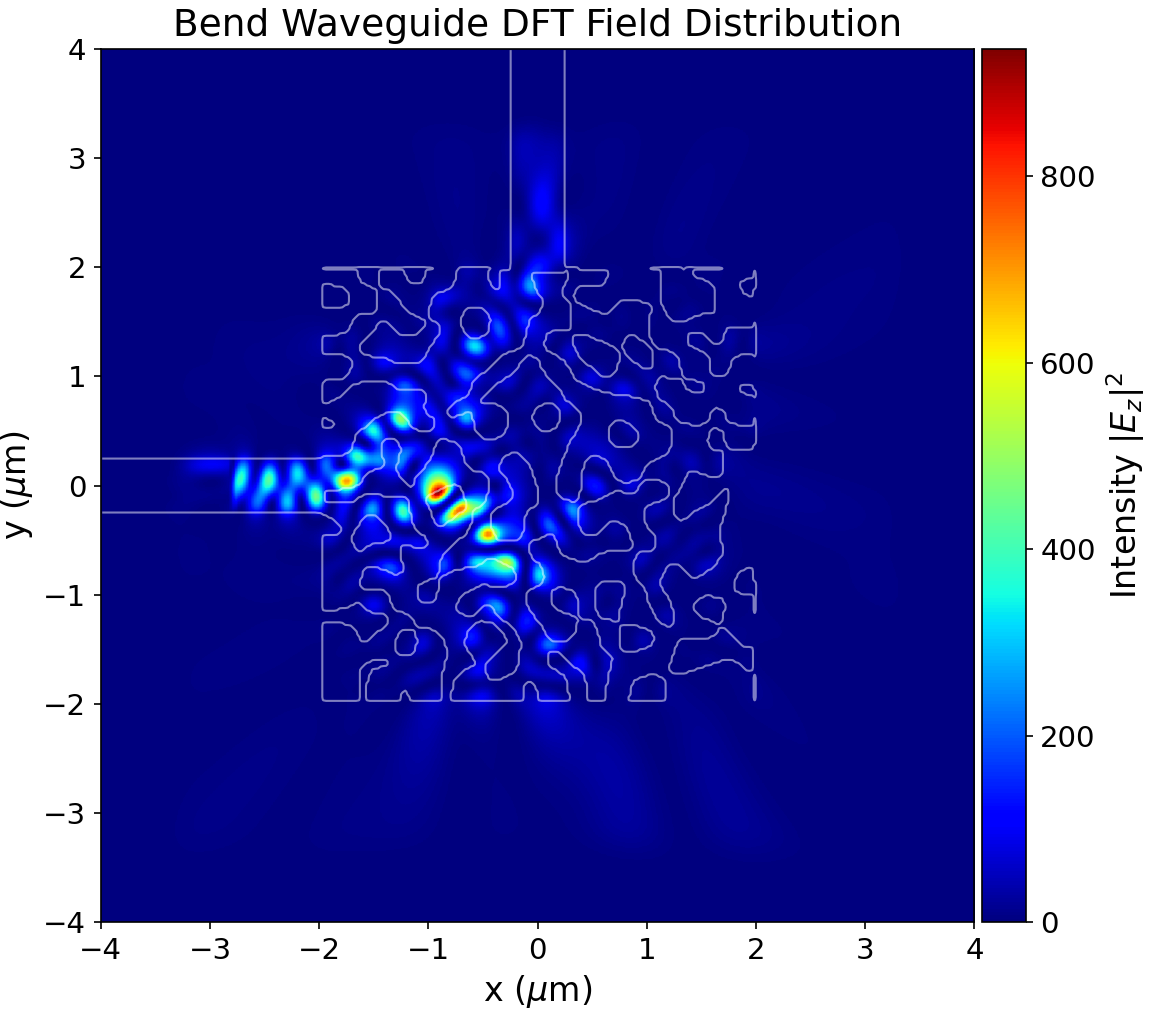
\includegraphics[width=0.8\textwidth]{img/BEND/BEND-2F-design5/final_analysis_TE0_field.png}
\caption{二維傅立葉積分策略應用於彎曲波導 Design 5之DFT電場強度分布圖。}
\label{fig:BEND_2F_DFT_design5}
\end{figure}

\begin{figure}[H]
\centering
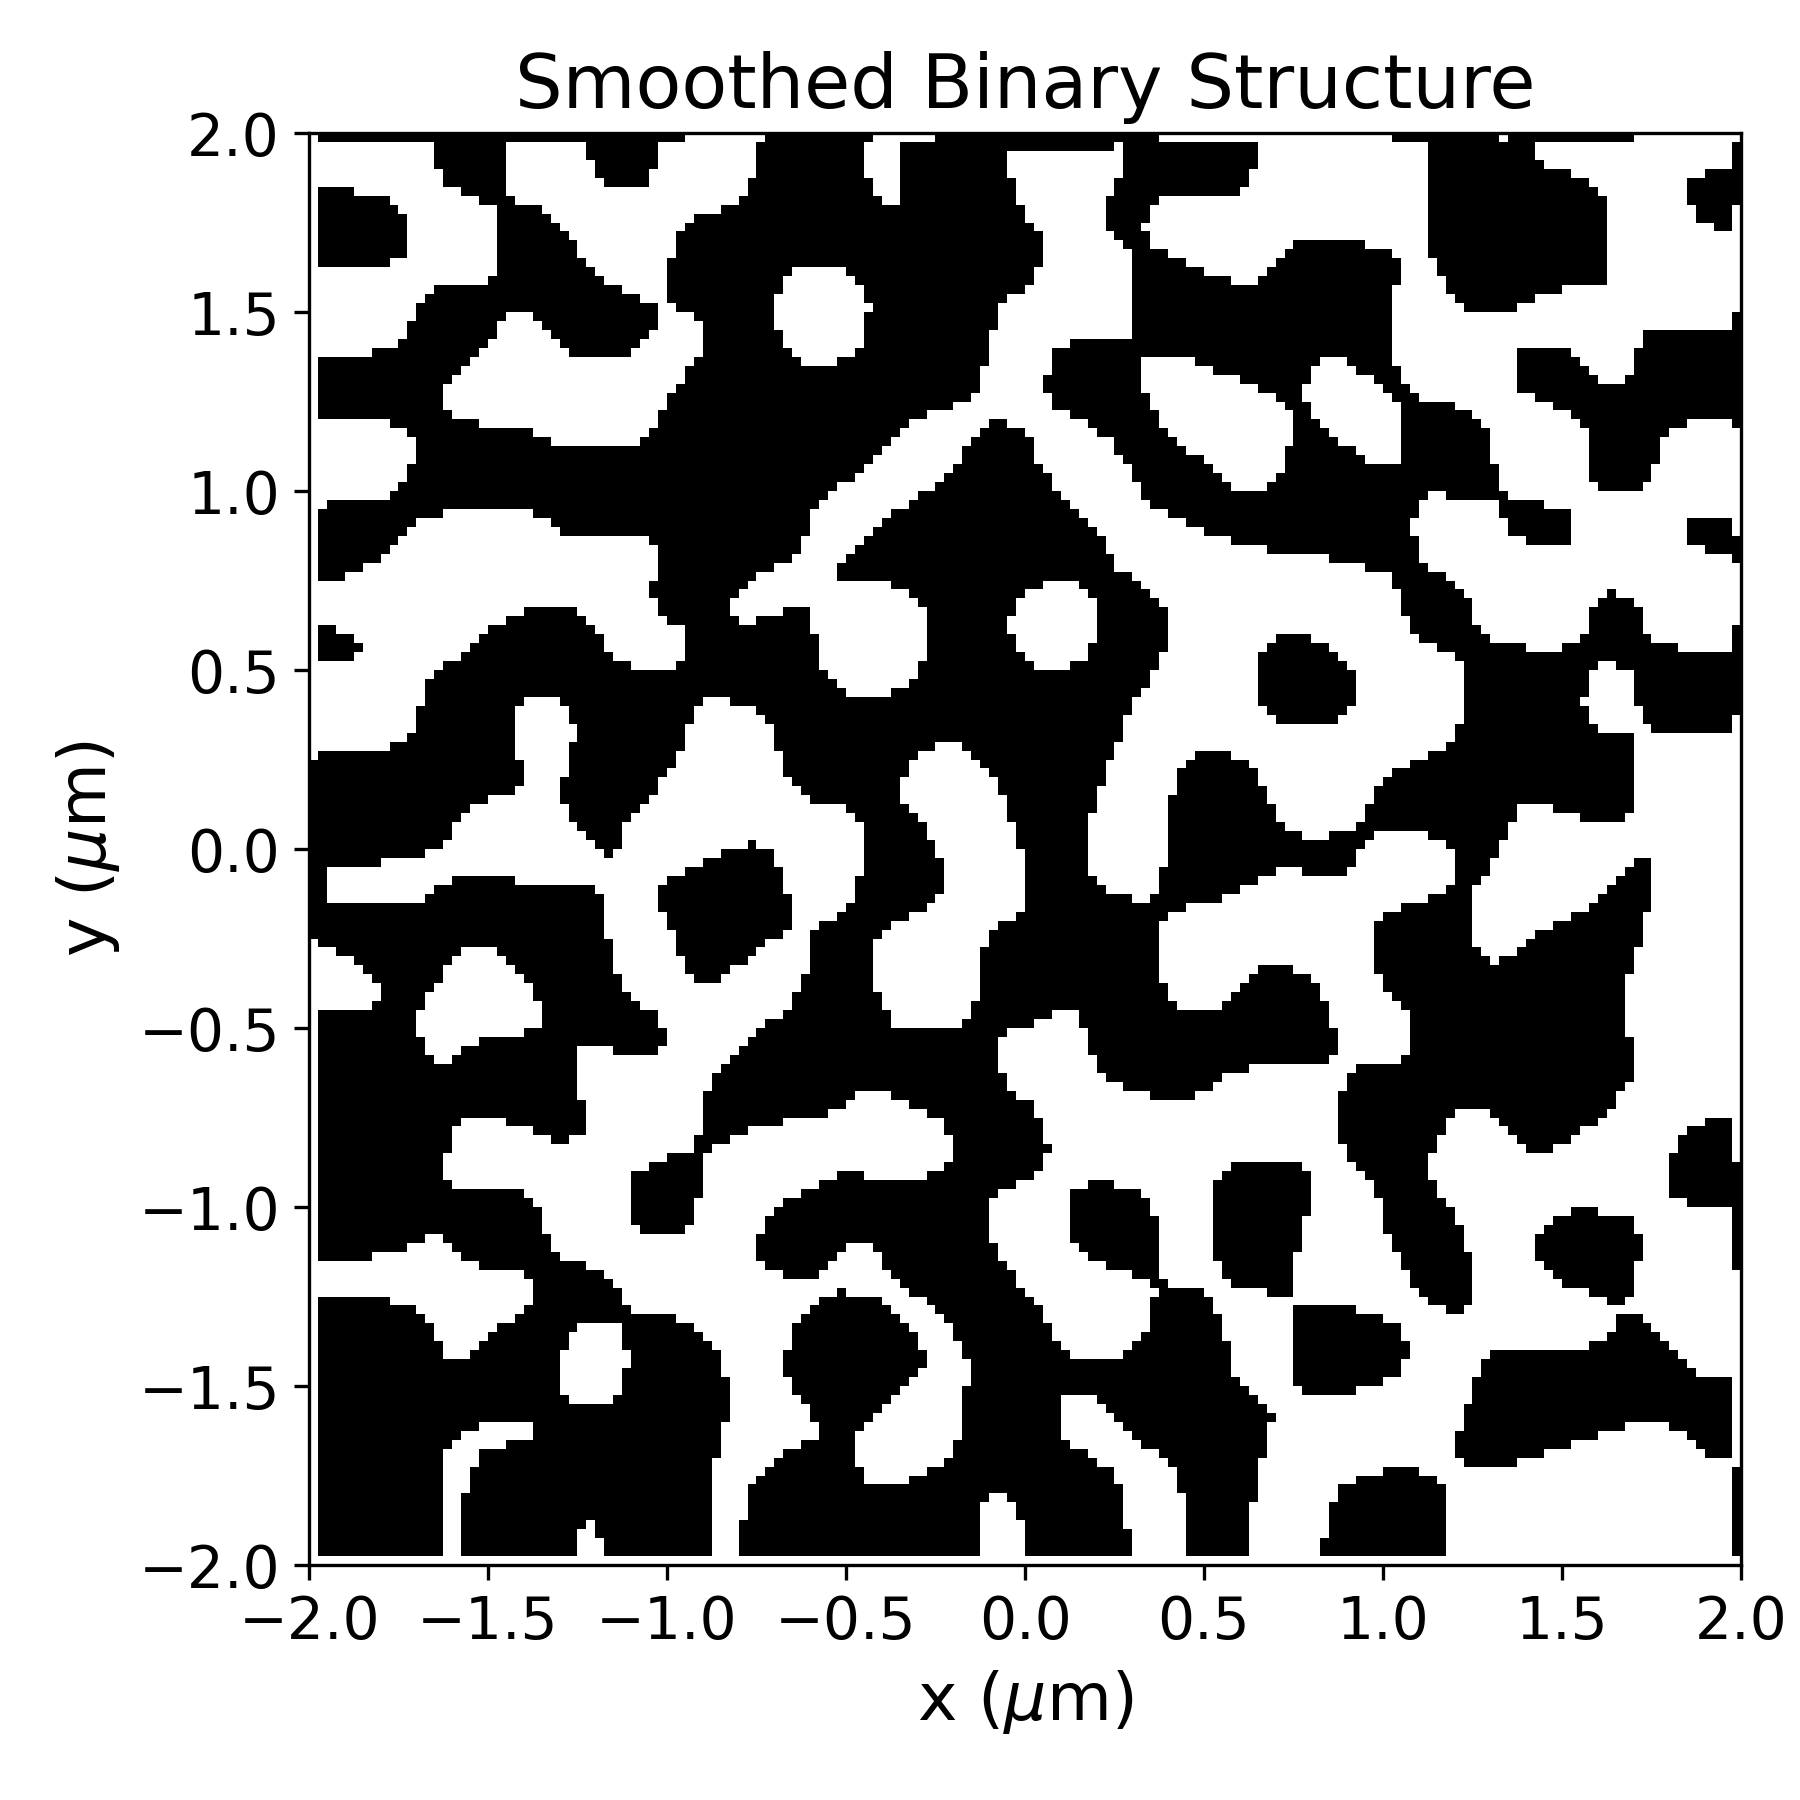
\includegraphics[width=0.7\textwidth]{img/BEND/BEND-2F-design5/Smoothed_Binary_Structure.png}
\caption{二維傅立葉積分策略應用於彎曲波導 Design 5之幾何結構圖。}
\label{fig:BEND_2F_structure_design5}
\end{figure}

\subsection{$\beta$-VAE on Bend Waveguide Design}
\subsubsection{$\beta$-VAE on Bend Waveguide Design - parameter 1}
\subsubsection{$\beta$-VAE on Bend Waveguide Design - parameter 2}
\subsubsection{$\beta$-VAE on Bend Waveguide Design - parameter 3}
\subsubsection{$\beta$-VAE on Bend Waveguide Design - parameter 4}



\section{Waveguide Crossing Optimization Results}

\subsection{Gaussian Upsampling Strategy on Waveguide Crossing Design}

\subsubsection{Gaussian Upsampling Strategy on Waveguide Crossing Design - parameter 1}
\subsubsection{Gaussian Upsampling Strategy on Waveguide Crossing Design - parameter 2}
\subsubsection{Gaussian Upsampling Strategy on Waveguide Crossing Design - parameter 3}
\subsubsection{Gaussian Upsampling Strategy on Waveguide Crossing Design - parameter 4}
\subsubsection{Gaussian Upsampling Strategy on Waveguide Crossing Design - parameter 5}

\subsubsection{Gaussian Upsampling Strategy on Waveguide Crossing Design - parameter 6}
\subsubsection{Gaussian Upsampling Strategy on Waveguide Crossing Design - parameter 7}



